\documentclass[12pt,a4paper,titlepage,twoside,openright]{book}
\makeatletter\if@twocolumn\PassOptionsToPackage{switch}{lineno}\else\fi\makeatother

\usepackage[utf8x]{inputenc}
\usepackage{tabulary,amsfonts,amsmath,amssymb,color,amsbsy,amstext,graphicx}%%
\usepackage{fixltx2e}
\usepackage{abstract}

\usepackage[mathscr]{eucal}
\usepackage[T1]{fontenc}
\usepackage[section]{placeins}


% --------------------
% Lists and references
% --------------------
\usepackage[linktoc=all]{hyperref}
\hypersetup{
    colorlinks,
    citecolor=black,
    filecolor=black,
    linkcolor=black,
    urlcolor=black
}

% bibliography at the end of every chapter
\usepackage[numbers,sort&compress,sectionbib,square]{natbib}
\usepackage{chapterbib}

% List of index
\usepackage{makeidx}
\makeindex

% Glossary --> defitions of symbols and acronyms
%\usepackage[toc,nonumberlist,nopostdot]{glossaries}
%\makeglossaries
%\setglossarystyle{treegroup}

% ------
% Layout
% ------

% Suppress "This page intentionally left blank."
\newcommand*\markblankpages{}

% set page margins
%   these margins are set by the A4 paper ratios, 1:sqrt(2)
%   paperheight/paperwidth = paperwidth/textwidth = paperheight/textheight = sqrt(2)
%   outer/inner = bottom/top = sqrt(2)
\usepackage[outer=36.02988mm,inner=25.47697mm,top=36.0317mm,bottom=50.9565mm]{geometry}
\newcommand*\symmetricmargin{
    \newgeometry{outer=30.7534mm,inner=30.7534mm,top=36.0317mm,bottom=50.9565mm}
}
\newcommand*\bookmargin{
    \newgeometry{outer=36.02988mm,inner=25.47697mm,top=36.0317mm,bottom=50.9565mm}
}

% we've already gone this far, why not go the whole mile
% set the text spacing 
\renewcommand{\baselinestretch}{1.5}

% For testing the formatting
\usepackage{lipsum}

% ---------
% Eye candy
% ---------

\usepackage{setspace}
\usepackage[labelfont={bf,singlespacing},
            textfont={singlespacing},
            justification={justified,RaggedRight},
            singlelinecheck=false,
            margin=0pt,
            figurewithin=chapter,
            tablewithin=chapter]{caption}
    

%\usepackage[titletoc]{appendix}

% fancy chapter titles and quotes at beginning of title
\usepackage[helvetica]{quotchap} 

% Draft watermark
\usepackage[contents={}]{background}
\usepackage[yyyymmdd,hhmmss]{datetime}
\newcommand*\DraftText{Draft compiled on \today\ at \currenttime}
\newcommand*\draft{
  \newcommand*{\archivalpapernote}{}
  \backgroundsetup{
    color=lightgray,
    position=current page.center,
    angle=90,
    vshift=0.45\paperwidth,
    opacity=1,
    scale=1,
    contents={\LARGE\ttfamily\DraftText}
  }
}

\newcommand*\myglossaryentry[4]{
    \index{#2@#1}
    \newglossaryentry{#2}{name={#1}, description={#3}, sort={#2}, #4}
}

\newcommand*\myacronym[2]{
    \index{#1}
    \newacronym{#1}{#1}{#2}
}

% clear to the start of a right-hand page (top)
\newcommand*\cleartorightpage{
    \cleardoublepage
}

% clear to the start of a left-hand page (rev)
\newcommand*\cleartoleftpage{
    \clearpage
    \ifodd\value{page}\hbox{}\newpage\fi
}


%%%%%%%%%%%%%%%%%%%%%%%%%%%%%%%%%%%%%%%%%%%%%%%%%%%%%%%%%%%%%%%%%%%%%%%%%%
% Following additional macros are required to function some 
% functions which are not available in the class used.
%%%%%%%%%%%%%%%%%%%%%%%%%%%%%%%%%%%%%%%%%%%%%%%%%%%%%%%%%%%%%%%%%%%%%%%%%%
\usepackage{url,multirow,morefloats,floatflt,cancel,tfrupee}
\makeatletter


\AtBeginDocument{\@ifpackageloaded{textcomp}{}{\usepackage{textcomp}}}
\makeatother
\usepackage{colortbl}
\usepackage{xcolor}
\usepackage{pifont}
\usepackage[nointegrals]{wasysym}
\urlstyle{rm}
\makeatletter

%%%For Table column width calculation.
\def\mcWidth#1{\csname TY@F#1\endcsname+\tabcolsep}

%%Hacking center and right align for table
\def\cAlignHack{\rightskip\@flushglue\leftskip\@flushglue\parindent\z@\parfillskip\z@skip}
\def\rAlignHack{\rightskip\z@skip\leftskip\@flushglue \parindent\z@\parfillskip\z@skip}

%Etal definition in references
\@ifundefined{etal}{\def\etal{\textit{et~al}}}{}


%\if@twocolumn\usepackage{dblfloatfix}\fi
\usepackage{ifxetex}
\ifxetex\else\if@twocolumn\@ifpackageloaded{stfloats}{}{\usepackage{dblfloatfix}}\fi\fi

\AtBeginDocument{
\expandafter\ifx\csname eqalign\endcsname\relax
\def\eqalign#1{\null\vcenter{\def\\{\cr}\openup\jot\m@th
  \ialign{\strut$\displaystyle{##}$\hfil&$\displaystyle{{}##}$\hfil
      \crcr#1\crcr}}\,}
\fi
}

%For fixing hardfail when unicode letters appear inside table with endfloat
\AtBeginDocument{%
  \@ifpackageloaded{endfloat}%
   {\renewcommand\efloat@iwrite[1]{\immediate\expandafter\protected@write\csname efloat@post#1\endcsname{}}}{\newif\ifefloat@tables}%
}%

\def\BreakURLText#1{\@tfor\brk@tempa:=#1\do{\brk@tempa\hskip0pt}}
\let\lt=<
\let\gt=>
\def\processVert{\ifmmode|\else\textbar\fi}
\let\processvert\processVert

\@ifundefined{subparagraph}{
\def\subparagraph{\@startsection{paragraph}{5}{2\parindent}{0ex plus 0.1ex minus 0.1ex}%
{0ex}{\normalfont\small\itshape}}%
}{}

% These are now gobbled, so won't appear in the PDF.
\newcommand\role[1]{\unskip}
\newcommand\aucollab[1]{\unskip}
  
\@ifundefined{tsGraphicsScaleX}{\gdef\tsGraphicsScaleX{1}}{}
\@ifundefined{tsGraphicsScaleY}{\gdef\tsGraphicsScaleY{.9}}{}
% To automatically resize figures to fit inside the text area
\def\checkGraphicsWidth{\ifdim\Gin@nat@width>\linewidth
	\tsGraphicsScaleX\linewidth\else\Gin@nat@width\fi}

\def\checkGraphicsHeight{\ifdim\Gin@nat@height>.9\textheight
	\tsGraphicsScaleY\textheight\else\Gin@nat@height\fi}

\def\fixFloatSize#1{}%\@ifundefined{processdelayedfloats}{\setbox0=\hbox{\includegraphics{#1}}\ifnum\wd0<\columnwidth\relax\renewenvironment{figure*}{\begin{figure}}{\end{figure}}\fi}{}}
\let\ts@includegraphics\includegraphics

\def\inlinegraphic[#1]#2{{\edef\@tempa{#1}\edef\baseline@shift{\ifx\@tempa\@empty0\else#1\fi}\edef\tempZ{\the\numexpr(\numexpr(\baseline@shift*\f@size/100))}\protect\raisebox{\tempZ pt}{\ts@includegraphics{#2}}}}

%\renewcommand{\includegraphics}[1]{\ts@includegraphics[width=\checkGraphicsWidth]{#1}}
\AtBeginDocument{\def\includegraphics{\@ifnextchar[{\ts@includegraphics}{\ts@includegraphics[width=\checkGraphicsWidth,height=\checkGraphicsHeight,keepaspectratio]}}}

\DeclareMathAlphabet{\mathpzc}{OT1}{pzc}{m}{it}

\def\URL#1#2{\@ifundefined{href}{#2}{\href{#1}{#2}}}

%%For url break
\def\UrlOrds{\do\*\do\-\do\~\do\'\do\"\do\-}%
\g@addto@macro{\UrlBreaks}{\UrlOrds}



\edef\fntEncoding{\f@encoding}
\def\EUoneEnc{EU1}
\makeatother
\def\floatpagefraction{0.8} 
\def\dblfloatpagefraction{0.8}
\def\style#1#2{#2}
\def\xxxguillemotleft{\fontencoding{T1}\selectfont\guillemotleft}
\def\xxxguillemotright{\fontencoding{T1}\selectfont\guillemotright}

\newif\ifmultipleabstract\multipleabstractfalse%
\newenvironment{typesetAbstractGroup}{}{}%

%%%%%%%%%%%%%%%%%%%%%%%%%%%%%%%%%%%%%%%%%%%%%%%%%%%%%%%%%%%%%%%%%%%%%%%%%%





\usepackage{float}

\begin{document}


\begin{frontmatter}
\frontmatterheadings

\title{~\mbox{}}\author{~}

\author{Katalina Bobowik}
\degree{}
\submissionyear{2019}
\submissionmonth{APRIL}
\department{Biosciences}\university{\scshape The University of Melbourne}
\symmetricmargin
\maketitle
\bookmargin

\begin{abstract}
Our understanding of function within the human genome has been largely limited to populations of European ancestry. In order to better characterise human functional diversity, this study aims to analyse regulatory variation in three isolated populations within the Indonesian archipelago. No study has yet analysed regulatory variation in Indonesia and the small, isolated nature of these populations makes them ideal to identify variants that have risen to higher frequencies. In this study, I identify variants influencing gene expression through the analysis of RNA sequencing data with a focus on pathways associated with immune function and disease.


\end{abstract}\makedeclaration 
{\singlespacing\tableofcontents\clearpage
\addcontentsline{toc}{chapter}{List of Figures}
\listoffigures\clearpage}

\end{frontmatter}
\begin{mainmatter}
\mainmatterheadings

\chapter{Introduction}\label{}
Humans, during their migration through diverse ecological settings, have experienced unique pathogenic and environmental pressures, consequently shaping genomes through microevolutionary processes. Although population genetic studies and genome-wide scans have provided new insight into the demographic and selection history of our species, the majority of variants found have been in non-coding regions of the genome (Albert and Kruglyak 2015; Zappala and Montgomery 2016; Pala et al. 2017) making the biological processes they affect difficult to identify. In the past decade, the endeavour to understand genome biology and function has been greatly aided by gene expression studies in which regulatory variants can be matched to RNA expression data. This has facilitated our understanding of complex traits (Cookson et al. 2009; Albert and Kruglyak 2015), enabled us to identify variants associated with genetic disease (Kremer et al. 2017), and understand the relationship between genetic variation and immune phenotypic diversity (Gupta et al. 2014; Chen et al. 2017). To date, the vast majority of these studies have focused on populations of primarily European descent. Given the diverse demographic history of our species, this fails to capture the full landscape of human regulatory variation (Quach et al. 2016; Martin et al. 2017). This study will focus on identifying regulatory variation in small, traditional populations of Southeast Asia in order to better understand phenotypic diversity and traits associated with immune function and disease. 

\section{Study group}\label{}
Our study groups come from three small island populations within Indonesia: Mentawai, Mappi, and Sumba. The first two islands, Mentawai and Mappi, capture two major genetic ancestries within Indonesia—Austronesians (Mentawai) and Melanesians (Mappi)—and also provide possible source populations to the last island, Sumba. This island is host to a network of traditional communities that derive from pre-existing Melanesians, arriving on the island ~50,000 years ago, and incoming Asian farming cultures, arriving ~4,000 years ago (Cox et al. 2016). These populations reside in tropical climates and face similar pathogenic pressures from vector borne, water borne, and water contact diseases. The fact that they share similar environments yet have different genetic ancestries is a unique opportunity to understand gene environment interactions and the effect of ancestry-related variation and its effect on immune gene expression.

\section{Previous studies analysing regulatory variation outside of Europe}
Although previous gene expression studies have identified factors influencing population-level variation in gene regulation (Battle et al. 2013; Westra et al. 2013), few have analysed them in non-European populations (Martin et al. 2014; Quach et al. 2016). One such study to analyse transcriptome variation across a globally distributed set of populations was performed by Martin et al. (2014). In this analysis, genome, exome, and transcriptome sequencing data for seven global populations was generated from lymphoblastoid cell lines derived from 45 individuals in the Human Genome Diversity Panel (4-7 samples per population). The authors found that approximately 25\%\ of the variation in gene expression could be attributed to population differences and were able to identify novel gene structures. Although the small sample size of the study lacked the power to detect additional population-specific variants, it highlighted the role of demography in understanding functional genetic variation. Furthermore, this is one of the only studies to analyse RNA sequencing (RNA-seq) data on a Southeast Asian population. The other such study to do so to our knowledge, and the only study to analyse RNA-seq data from a population within Indonesia, was conducted by Yamagishi et al (2014). This study analysed expression data collected from peripheral blood from 116 individuals infected with malaria. Despite having a population of over 260 million people, hosting hundreds of different ethnic groups, and covering the same area as continental Europe (Hudjashov et al. 2017), no study has analysed expression data from healthy Indonesian samples.

Along with a lack of studies analysing variation outside of Europe, most studies use large cohorts of well-studied populations for transcriptomic analysis. This fails to account for the genomic variation in small, structured populations that experience different evolutionary dynamics. Furthermore, small populations allow for the detection of rare variants that rise in frequency by chance, providing more statistical power for identification of functional alleles (Timpson et al. 2017). 

\section{Project significance and Aims}
Understanding how genes and regulatory networks operate is one of the biggest challenges in genomics and public health science. Not only do we have a limited understanding of the function of the human genome, but the regions we have characterised have been represented by only a small subset of all human genetic variation. Characterising this variation can ultimately lead to more accurate diagnosis and specific disease treatment, as well as a more thorough understanding of biological processes. Here, I analyses regulatory variation in 117 individuals who share similar environmental pressures yet have different ancestries in order to better understand how ancestry-related variation contributes to immune gene regulation.

\chapter{Methods}\label{}
\section{Sample collection and quality control}
A general overview of the differential expression pipeline is outlined in Figure \ref{fig:Study Pipeline}. Whole blood was collected by trained phlebotomists from the Eijkman Institute from over 300 Indonesian males. Samples were collected across multiple villages in the three islands using Tempus Blood RNA Tubes (Applied Biosystems) and extracted according to the manufacturer's protocol. We randomised all extraction and sequencing batches with respect to village and island. RNA quality was assessed with a Bioanalyzer 2100 (Agilent) and concentration through Qubit (Life Technologies). On the basis of these results, we selected the five villages in our study for having the highest average RIN and the largest number of individuals with a RIN >= 6.5. Library prep was done by Macrogen (South Korea), using 750ng of RNA and the Globin-Zero Gold rRNA Removal Kit (Illumina). 

\begin{figure}[htb!]
\centering
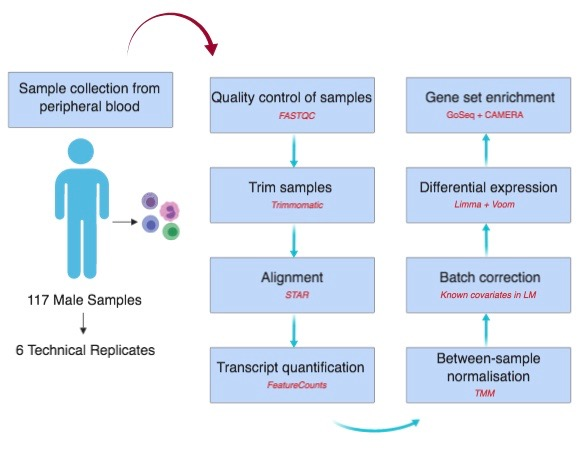
\includegraphics[width=\textwidth,height=\textheight,keepaspectratio]{Figures/SamplePipeline.jpg}
\caption{Peripheral blood samples from 117 Indonesian males (plus 6 technical replicates) were collected by trained phlebotomists from the Eijkman Institute. My sample pipeline consisted of an initial quality control step using FastQC, trimmiming samples using the software Trimmomatic, aligning reads using STAR, and then counting the number of transcripts using featureCounts. I used a Limma+Voom differential expression pipeline that used TMM normalisation for between-sample normalisation, batch correction incorporating covariates known to affect expression levels into a statistical model, and then gene ontology testing using GoSeq and Camera.}
\label{fig:Study Pipeline}
\end{figure}

101-bp paired-end reads were generated by Illumina sequencing (HiSeq 25000). This resulted in a total of 117 individuals, including six technical replicates (making a total of 123 sequences), sequenced in three batches (Supplementary Table 1). Upon data retrieval, all RNA sequencing reads went through an initial sample quality analysis using FastQC V0.11.5 (Babraham Institute, available for download at http://www.bioinformatics.babraham.ac.uk/projects/fastqc/). Base quality decreased near the 3’ end of reads, as is common with Illumina sequencing, and therefore all leading and trailing bases below a Phred quality score of 20 were removed using Trimmomatic version 0.36 (Bolger, Lohse, and Usadel 2014).

\section{Alignment and transcript quantification}
RNA-seq reads were aligned to the human genome (GrCh38, Ensembl release 90: August 2017) with STAR version 2.5.3a (Dobin et al. 2013). I used a two-pass alignment to improve identification of novel splice junctions which resulted in a mean of ~29 million uniquely-mapped read pairs per sample (Figure \ref{fig:Total and percentage of reads at all filtering stages}, Supplementary Table 2). Next, I performed read quantification with featureCounts version 1.5.3 (Liao, Smyth, and Shi 2014) and used a filtered GTF file for GRCh38.p10 that I created using the biomaRt R package. As some studies have suggested that prefiltering improves the performance of differential expression analysis by controlling the false discovery rate (Soneson et al. 2016), I set filtering parameters to only include GENCODE basic annotation and transcript support levels 1-3 (i.e., transcripts with at least one non-suspect mRNA or expressed sequence tag). Since many transcripts are poorly supported, this method provides a way of including transcript annotations that are actually expressed in humans. I used the default settings for featureCounts paired end reads, where features of exons are grouped into meta-features of genes. On average, I successfully assigned ~15 million paired-end reads to each sample (Figure \ref{fig:Total and percentage of reads at all filtering stages}, Supplementary Table 2). 

\begin{figure}[htb!]
\centering
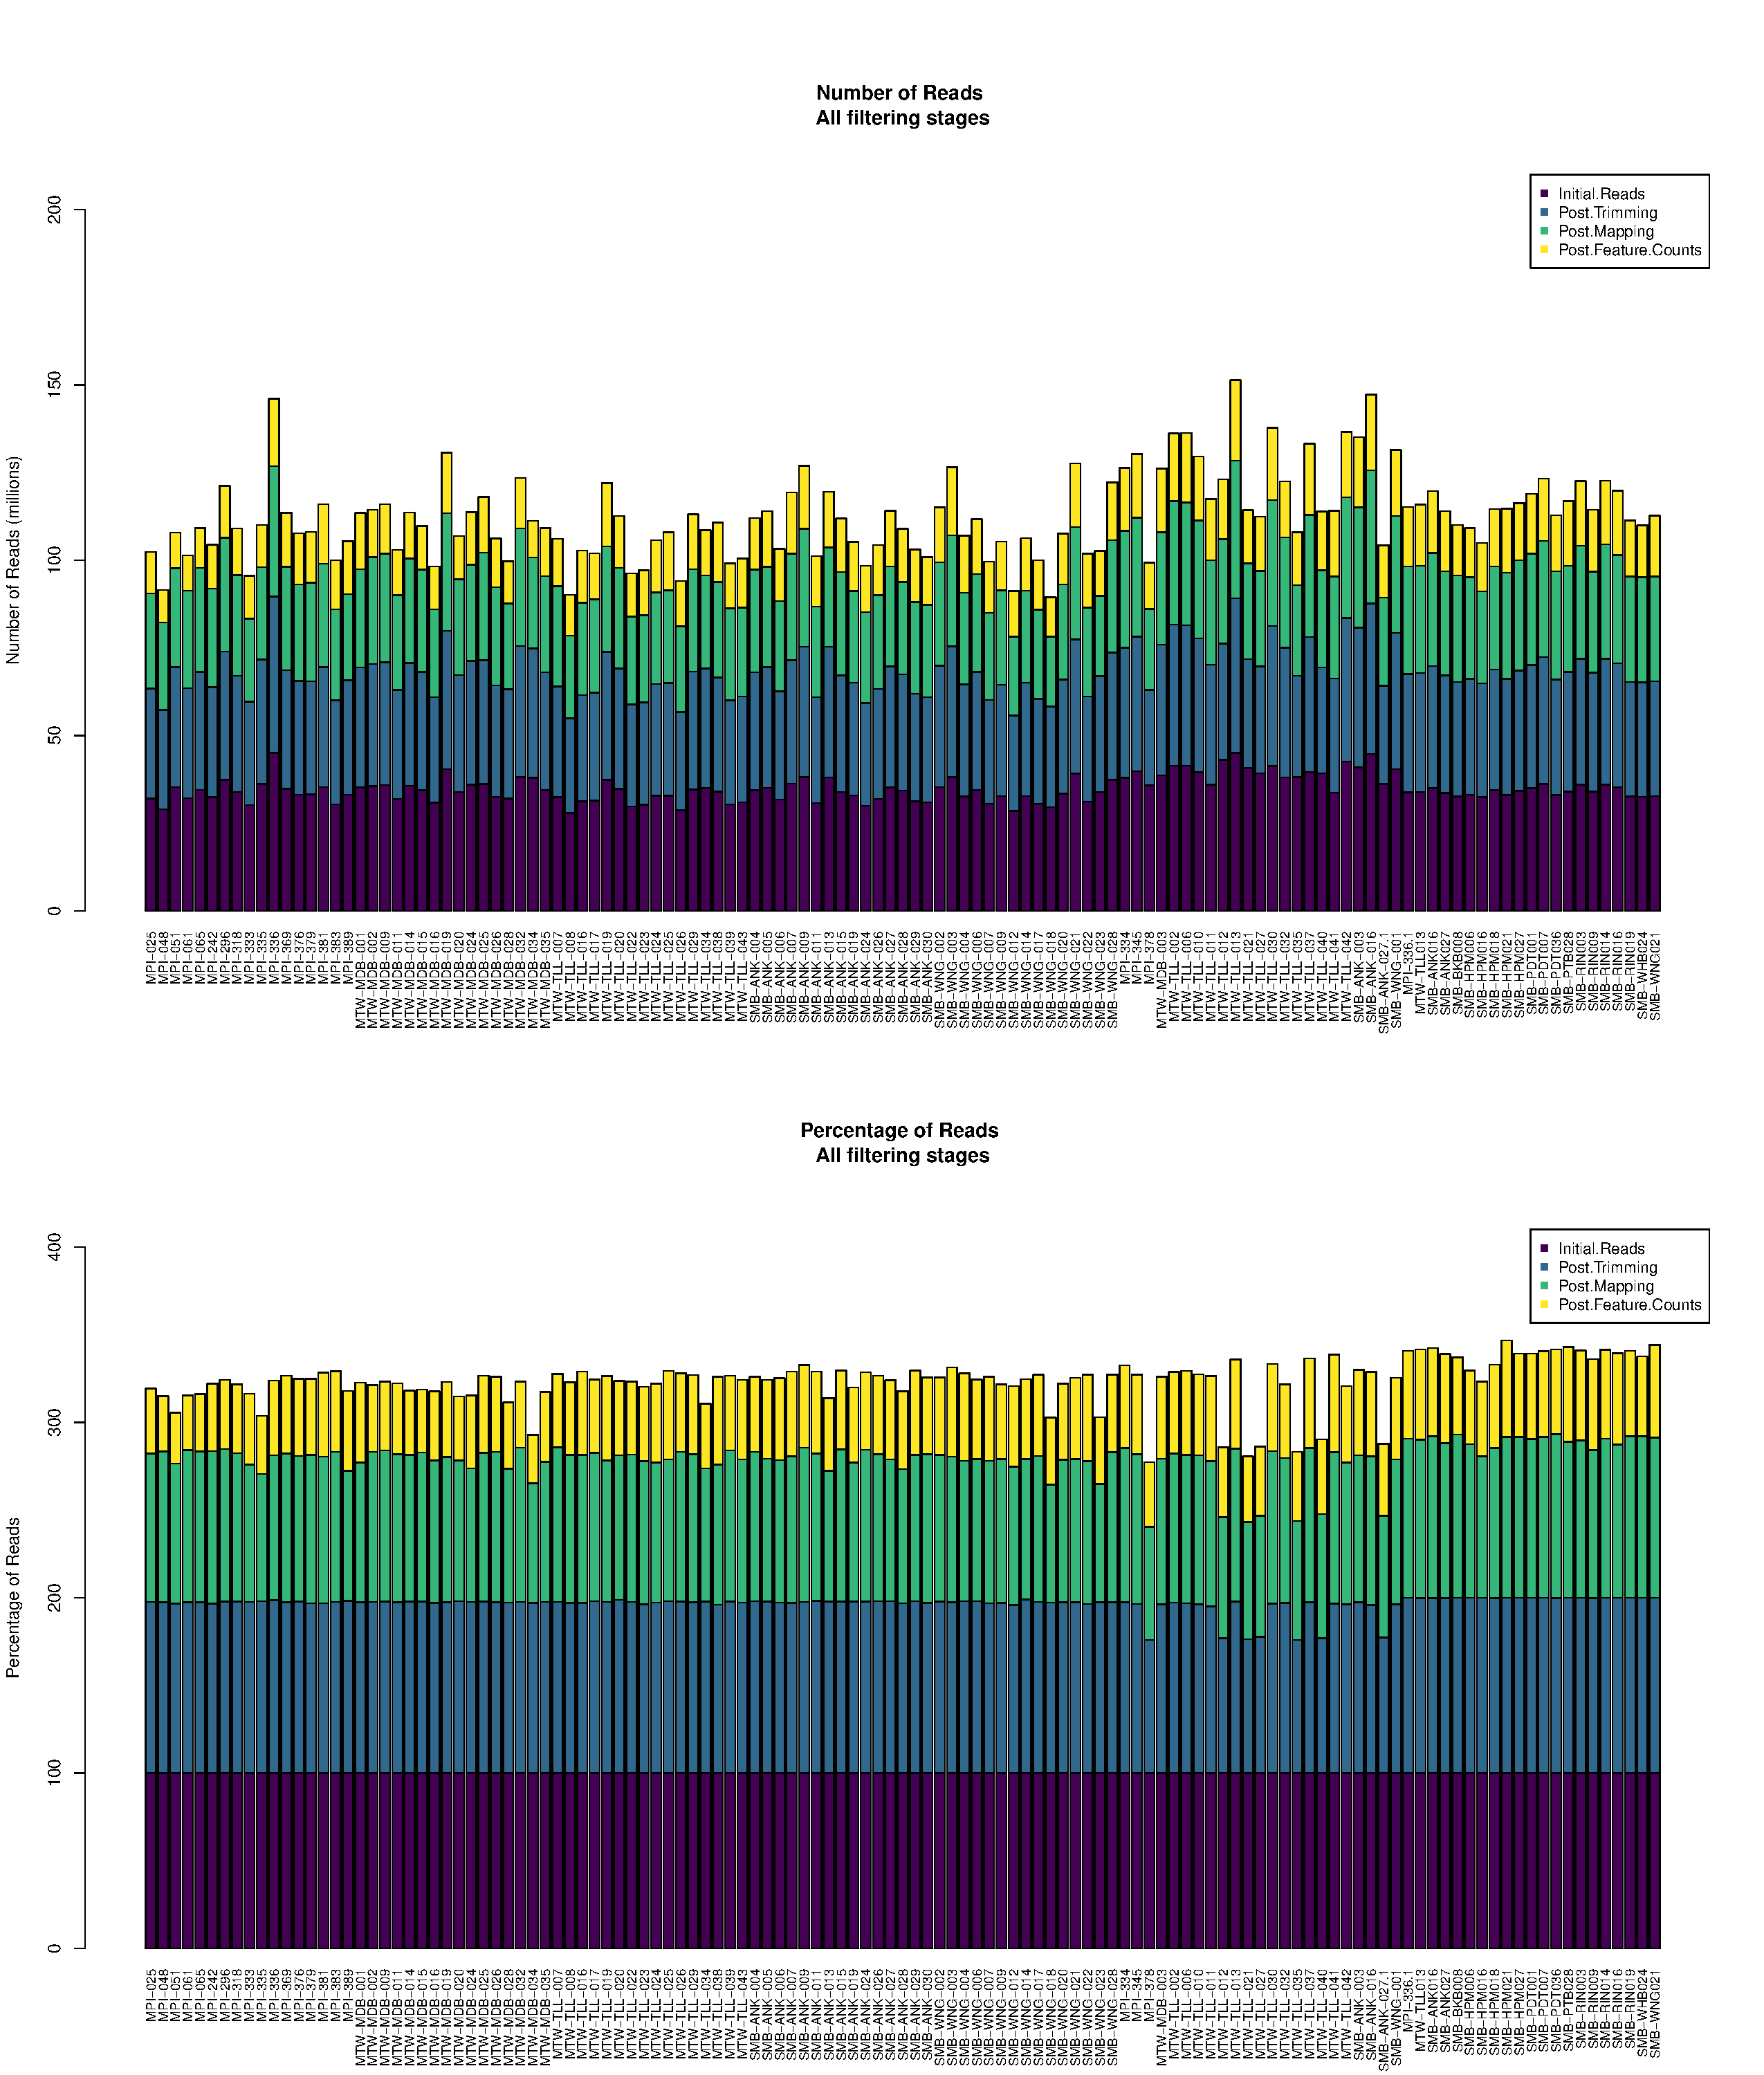
\includegraphics[width=\textwidth,height=\textheight,keepaspectratio]{Figures/TotalandPercentageOfReads_allFilteringStages.pdf}
\caption{Number (top) and percentage (bottom) of reads for each sample at each step of the RNASeq pipeline.}
\label{fig:Total and percentage of reads at all filtering stages}
\end{figure}

\section{Technical replicate analysis}
Six replicates were used in this study to ensure batch effects could be measured and removed: one sample was replicated twice in batches two and three (SMB-ANK-027) and the other four samples were replicated in batch three (MPI-381, MTW-TLL-013, SMB-ANK-016, SMB-WNG-021; Supplementary Table 1). I compared all samples to their corresponding replicate by plotting the correlation between the log2-CPM normalised counts after removal of lowly-expressed genes and then fitting a best-fit regression line (Figure \ref{fig:Replicate Comparisons}). The correlation between samples after log2 transformation and removal of lowly-expressed genes ranged from an R-squared value of 0.97-0.99, suggesting high similarity between all replicates.
\begin{figure}[h!]
\centering
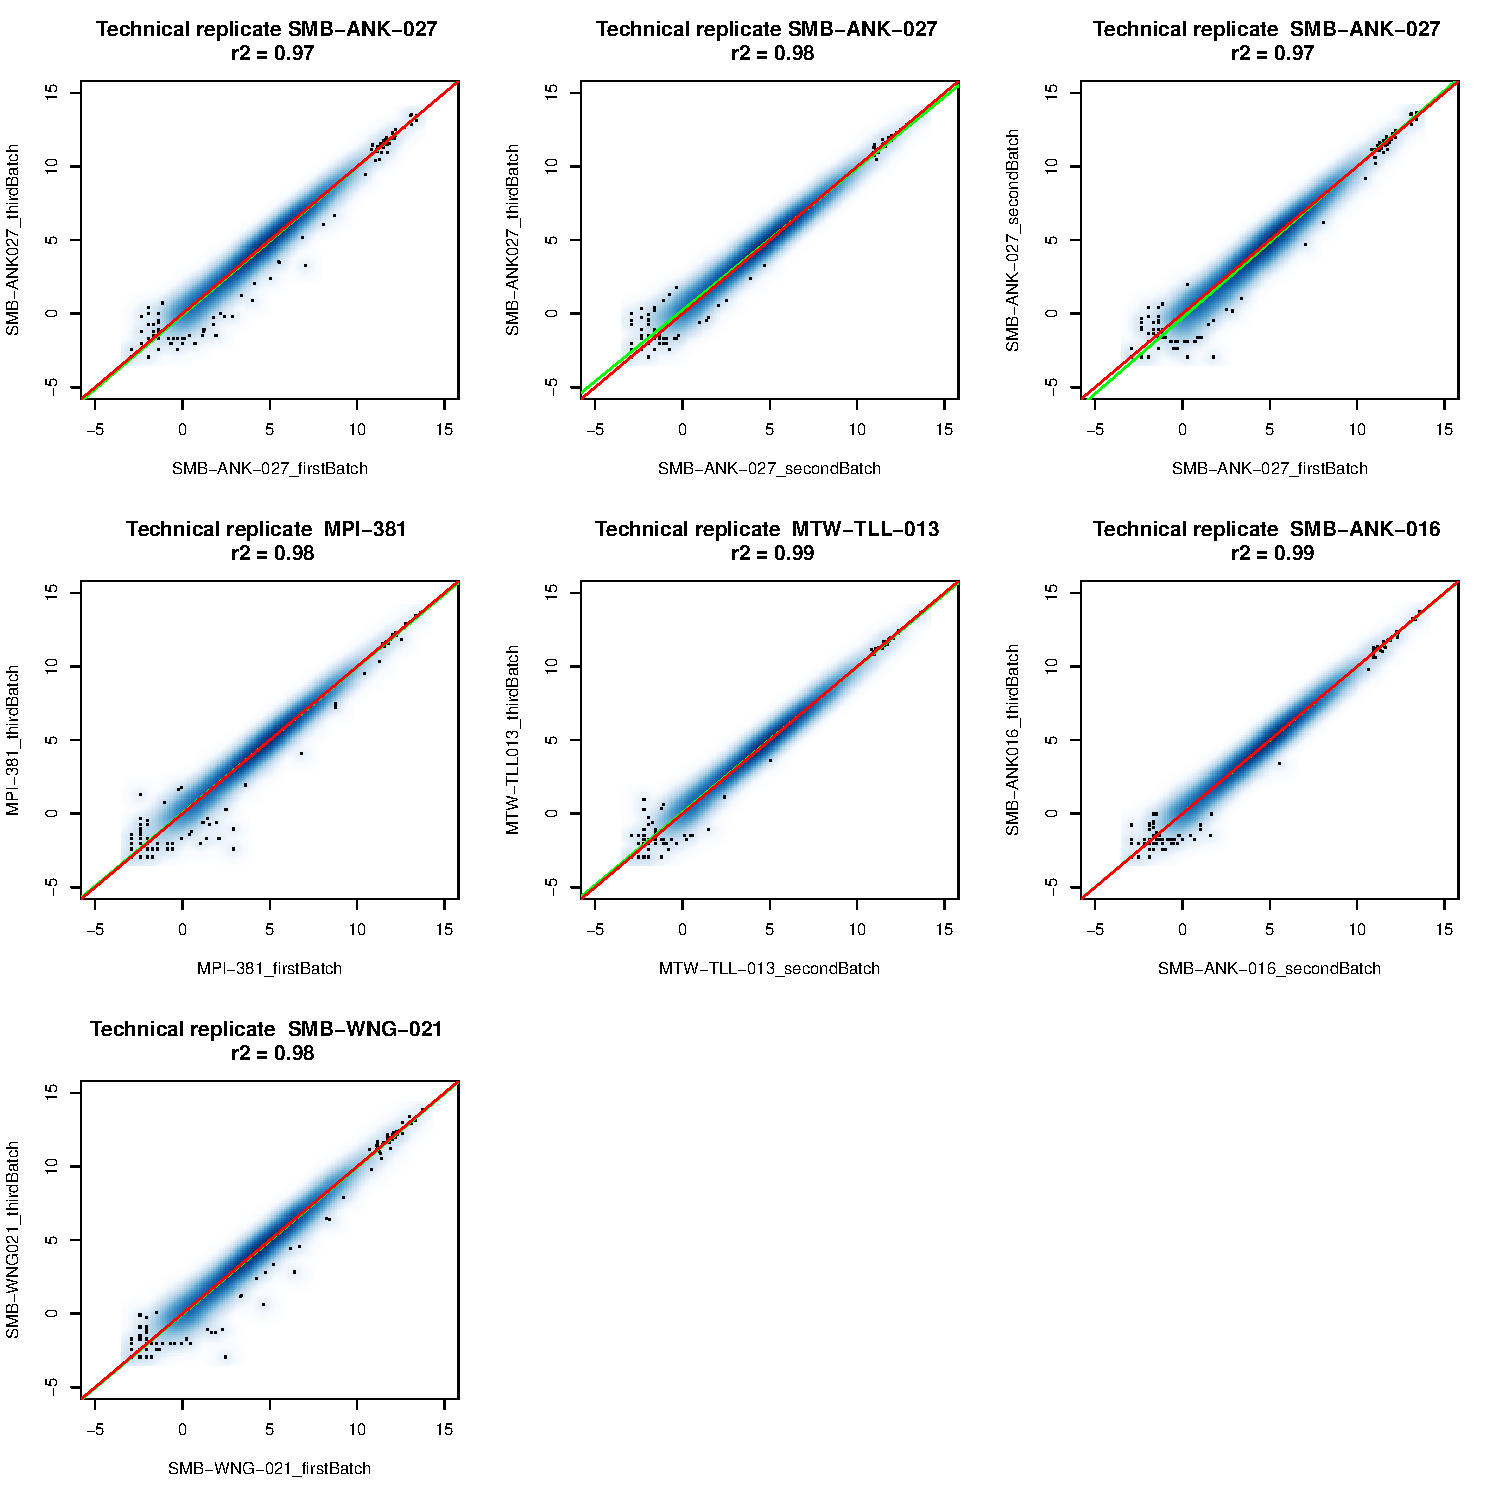
\includegraphics[width=\textwidth,height=\textheight,keepaspectratio]{Figures/replicate_comparisons_postFiltering_123Combined.pdf}
\caption{Performance of each control compared to its corresponding technical replicate sample after removal of lowly-expressed genes. All controls have one corresponding technical replicate with the exception of SMB-ANK-027, which has two (shown in panes 1, 2, and 3).}
\label{fig:Replicate Comparisons}
\end{figure}

\section{Removal of lowly-expressed genes and data normalization}
To account for library size differences, I transformed expression counts to log2-counts per million using a prior count of 0.25 in order to avoid taking the log of zero. I then removed lowly expressed genes by only keeping genes expressed at or over a CPM of one in at least one of the island groups, resulting in a total of 12,975 genes (Figure \ref{fig:library density after removal of lowly-expressed genes}, Supplementary Figure \ref{fig:Total Genes Post Filtering}). After filtering, sample library sizes ranged from roughly 9 million to 23 million reads (Figure \ref{fig:library size}).

\begin{figure}[htb!]
\centering
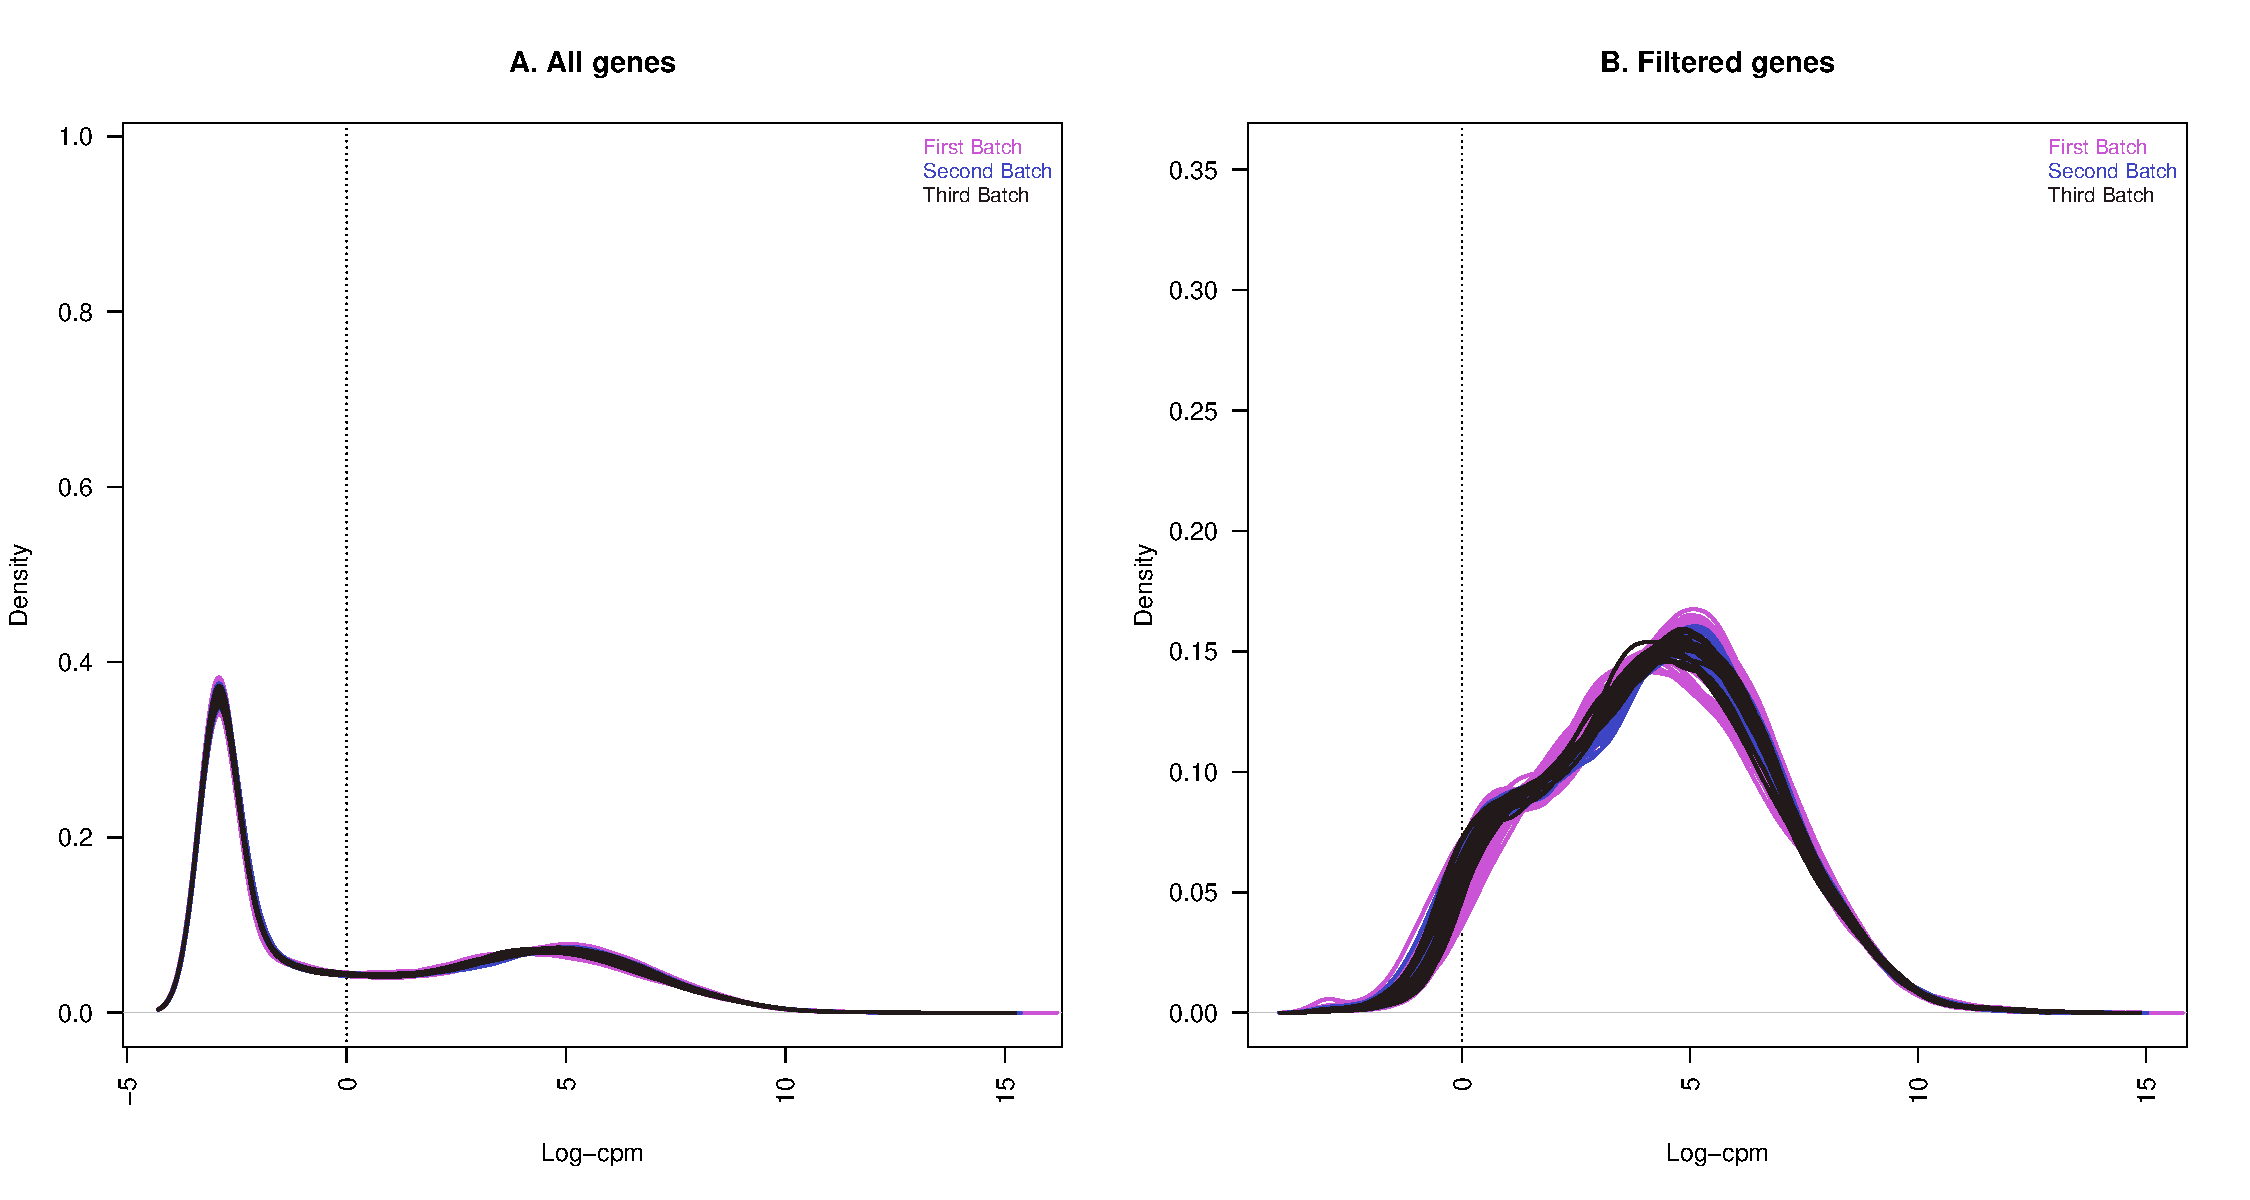
\includegraphics[width=\textwidth,height=\textheight,keepaspectratio]{Figures/libraryDensity_afterFiltering_indoRNA.pdf}
\caption{Gene expression distributions before and after filtering for lowly-expressed genes.The density of log2 counts per million (CPM) are shown for each sample with pink lines indicating samples from batch 1, purple lines indicating samples from batch 2, and black lines indicating samples from batch 3. The left panel shows data from 27,413 genes and the right panel shows data from 12,975 genes after filtering (i.e., only keeping genes expressed at or over a CPM of one in at least one of the island groups).}
\label{fig:library density after removal of lowly-expressed genes}
\end{figure}

In order to eliminate composition bias between libraries, I tested three different normalization methods: upperquartile, trimmed mean of M values (TMM), and relative log expression (RLE). Visual inspection of all three methods showed similar performance of normalization (Supplementary Figure \ref{fig:Testing Normalisation Methods}). A test of the TMM normalization was therefore chosen as it has been shown to have a low false discovery rate and high true positive rate (https://www.ncbi.nlm.nih.gov/pmc/articles/PMC5910605/). Furthermore, it is also recommended for RNA-Seq data where over half of the genes are not believed to be differentially expressed (edgeR manual: https://www.bioconductor.org/packages/devel/bioc/vignettes/edgeR/inst/doc/edgeRUsersGuide.pdf). In order to ensure composition bias was removed, I examined the performance of TMM-normalisation by plotting mean-difference (MD) plots for each sample. Most genes for each sample were centered around a log-fold change of zero, indicating that the composition bias was successfully removed (Figure \ref{fig:TMM normalisation}).

\begin{figure}[htb!]
\centering
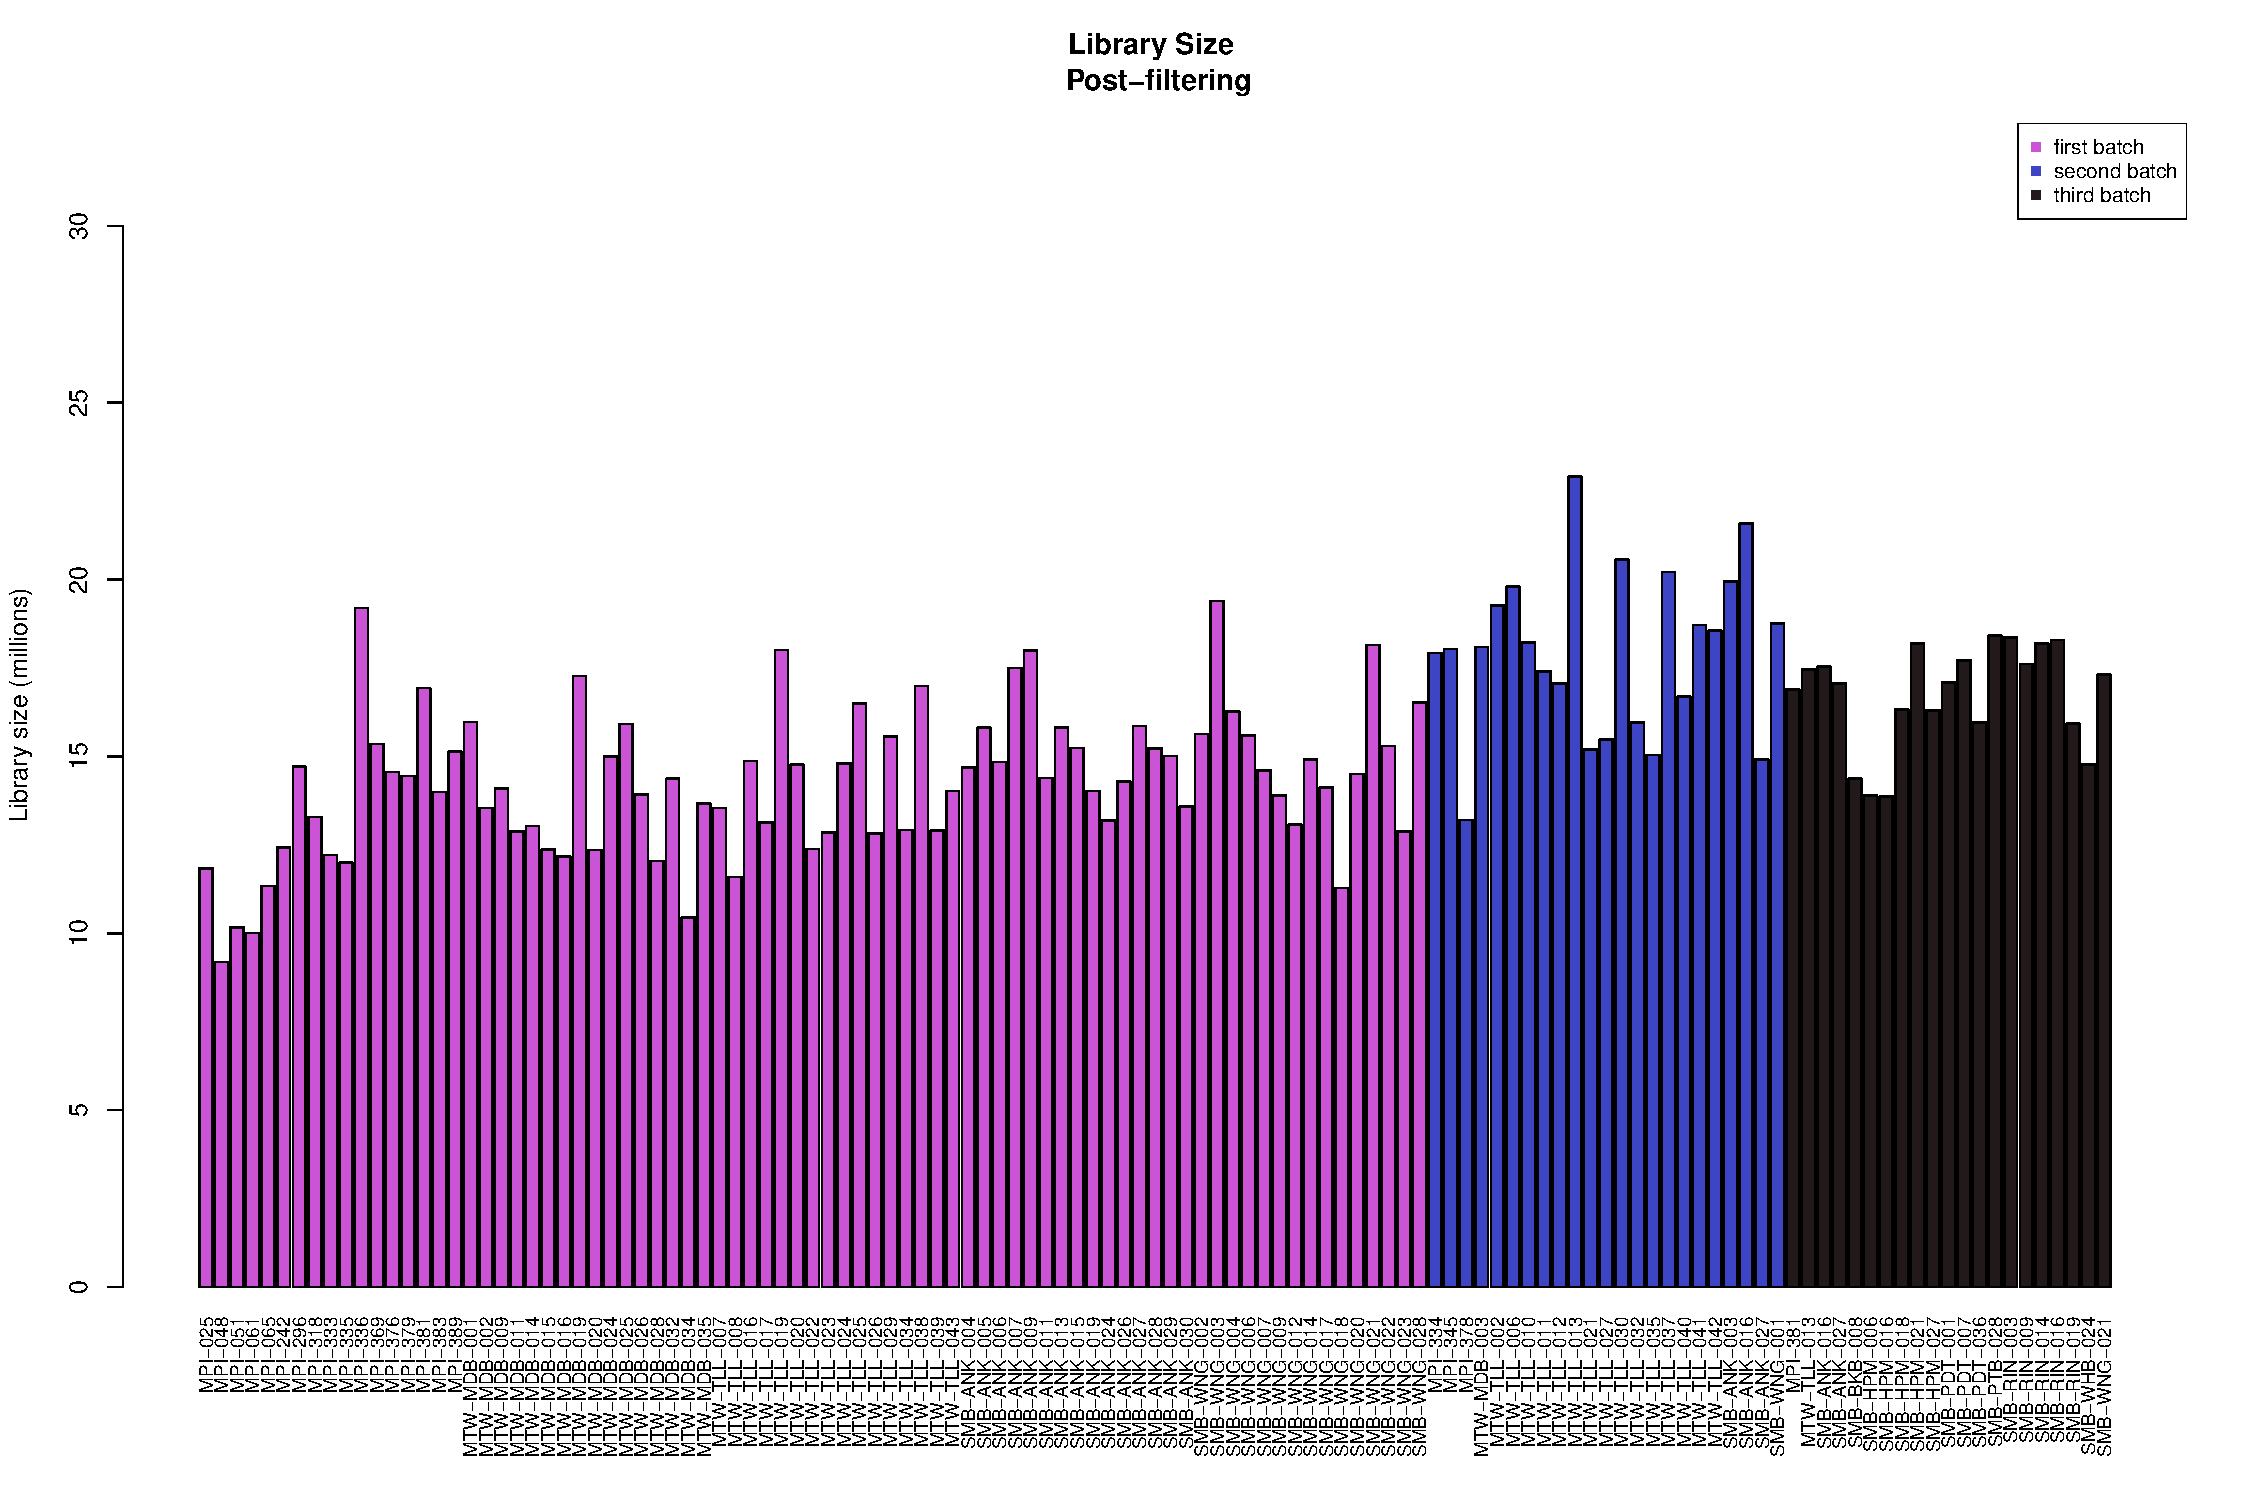
\includegraphics[width=\textwidth,height=\textheight,keepaspectratio]{Figures/librarySize_indoRNA_postFiltering_123Combined.pdf}
\caption{Total number of reads after filtering for lowly-expressed genes. The total library size ranged from 9 million 23 million read pairs.}
\label{fig:library size}
\end{figure}
  

\begin{figure}[htb!]
\centering
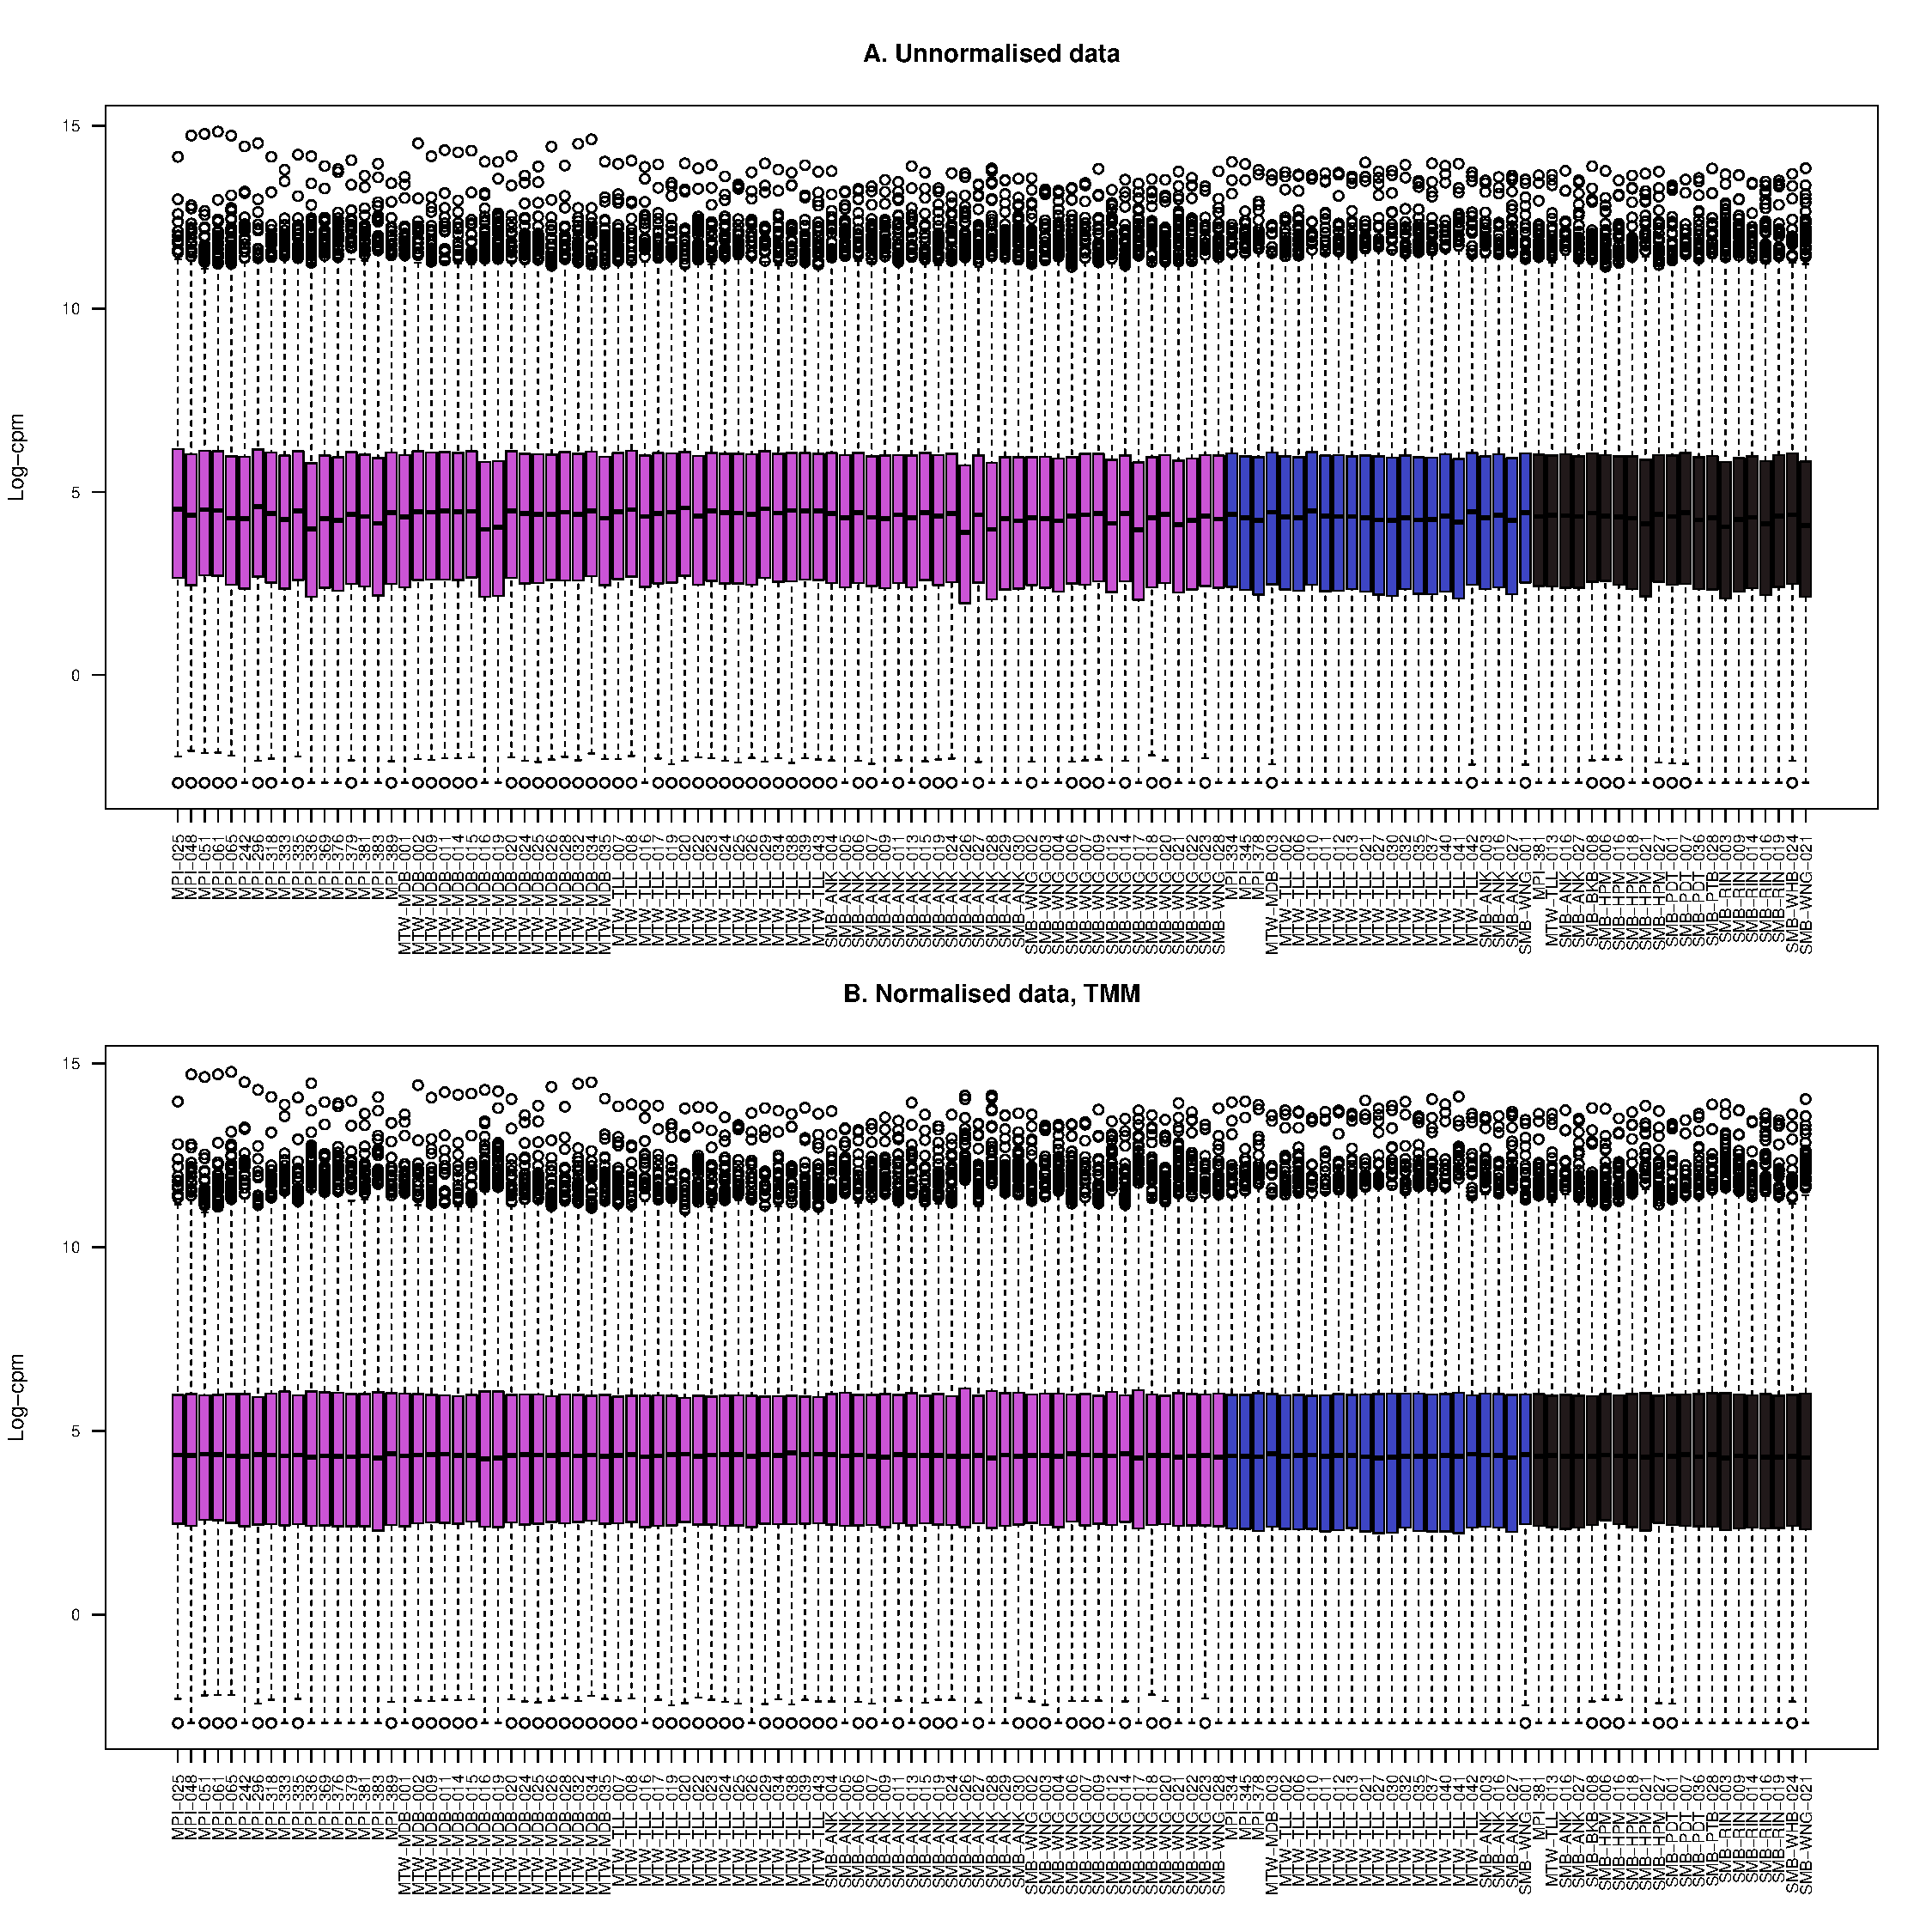
\includegraphics[width=\textwidth,height=\textheight,keepaspectratio]{Figures/NormalisedGeneExpressionDistribution_IndoRNA_TMM.pdf}
\caption{Performance of TMM normalisation on the log2-CPM transformed samples. Pink indicates sample from batch 1, purple indicates samples from batch 2, and black indicates samples from batch 3.}
\label{fig:TMM normalisation}
\end{figure}

\section{Sample variation analysis and data exploration}
In order to identify outlier samples and assess which covariates might be associated with expression levels, I used principal component analysis on the TMM-transformed log2 expression values (for a full list of covariates, see Supplementary Table 3). Associations between covariates and expression levels were analysed by inspecting the first ten dimensions in the data for clustering within each group. To identify significant associations (p<0.05) between covariates and expression levels, I performed ANOVA tests between covariates and each dimension of the PCA. The first PCA was most strongly associated with batch (Figure \ref{fig:PCA Batch}), followed by significant associations with island, RIN score, CD8T cells, and granulocytes (Figure \ref{fig:Significant Covariates}; for a full list of significant associations, see Supplementary Table 4). Sampling site, language, sampling date, sequencing pool, the Mappi tribe, and season also had significant associations, however these covariates were found to be confounded with other variables. In the second dimensions, blood cell type—in particular, granulocytes—had the highest correlation with expression levels. 

\begin{figure}[htb!]
\centering
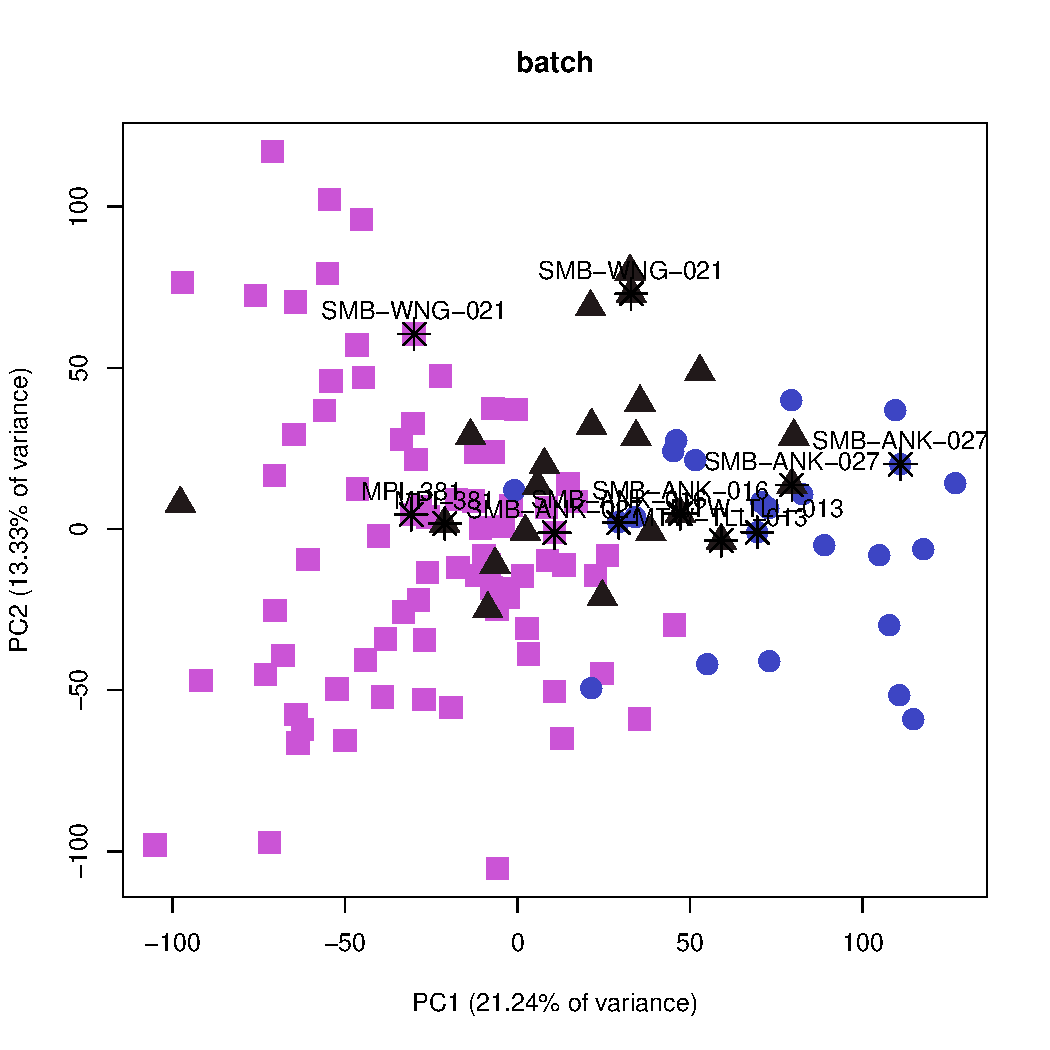
\includegraphics[width=\textwidth,height=\textheight,keepaspectratio]{Figures/pcaresults_batch.pdf}
\caption{Principal component analysis of the TMM-normalised, log2-transformed counts. Pink indicates sample from batch 1, purple indicates samples from batch 2, and black indicates samples from batch 3. Separation by batch can be seen in the first and second dimension of the PCA. Replicate samples are labelled with stars.}
\label{fig:PCA Batch}
\end{figure}

\begin{figure}[htb!]
\centering
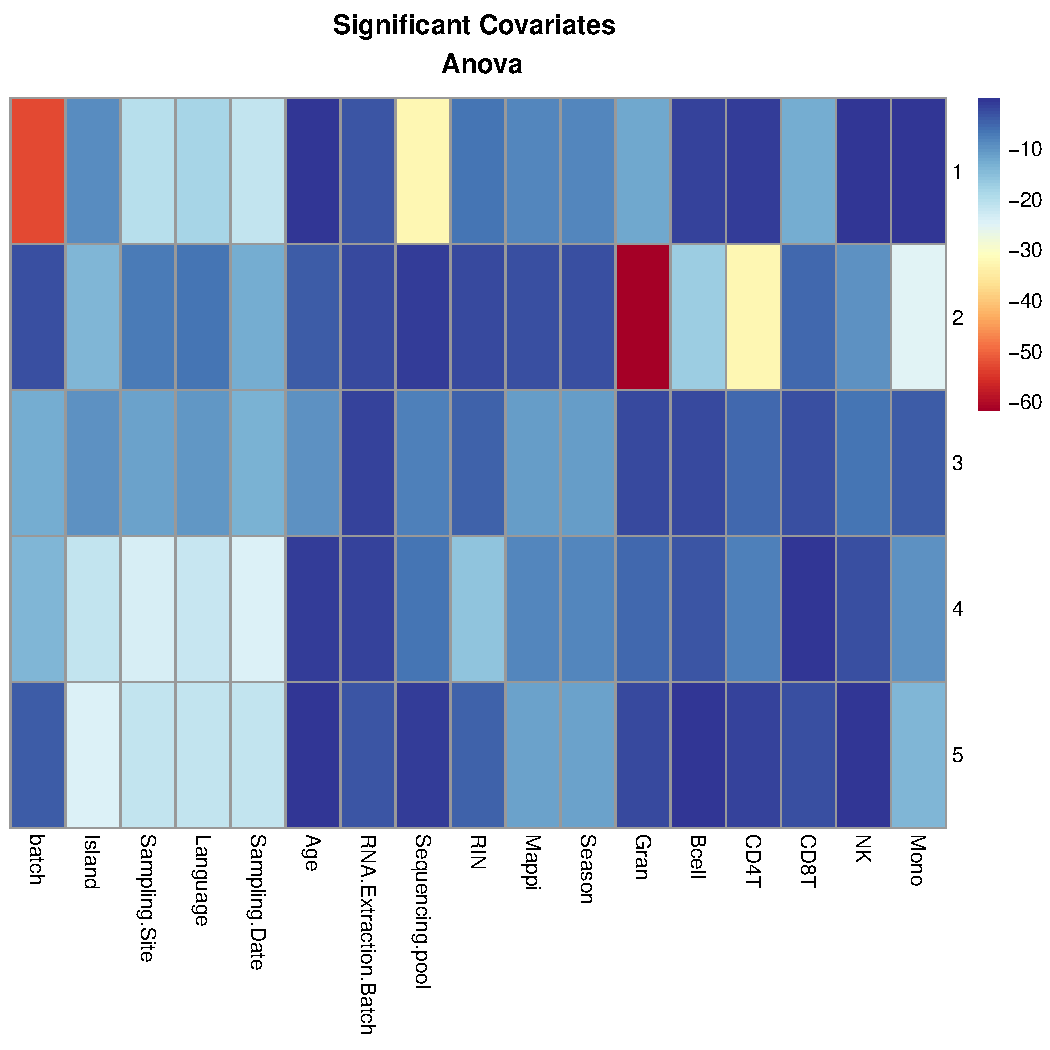
\includegraphics[width=\textwidth,height=\textheight,keepaspectratio]{Figures/significantCovariates_AnovaHeatmap.pdf}
\caption{Heatmap of significant covariates of the first 5 PCA dimensions(p=0.05). The covariate that had the strongest association with expression levels was batch, followed by granulocytes, CD8T cells, island, and RIN score.In the second dimension, all blood cell types(CD8T, CD4T, NK, B cells, monocytes, granulocytes) and island had the highest correlation with expression levels.}
\label{fig:Significant Covariates}
\end{figure}

Hierarchical clustering by Euclidean on the TMM-normalised, log2-transformed samples was performed in order to identify any sample outliers and analyse sample grouping (Figure \ref{fig:Euclidean Sample Distances}). Samples were shown to mostly cluster by island and no clear outliers were identified. Furthermore, between and within-island variation was analysed using Pearson correlations between log2-CPM expression values of samples (Figure 1\ref{fig:Island Variation}). As expected, most variation was seen between islands. Mappi was shown to have the highest amount of within-island variation and island populations compared to Mappi also had a higher degree of variation. 

\begin{figure}[htb!]
\centering
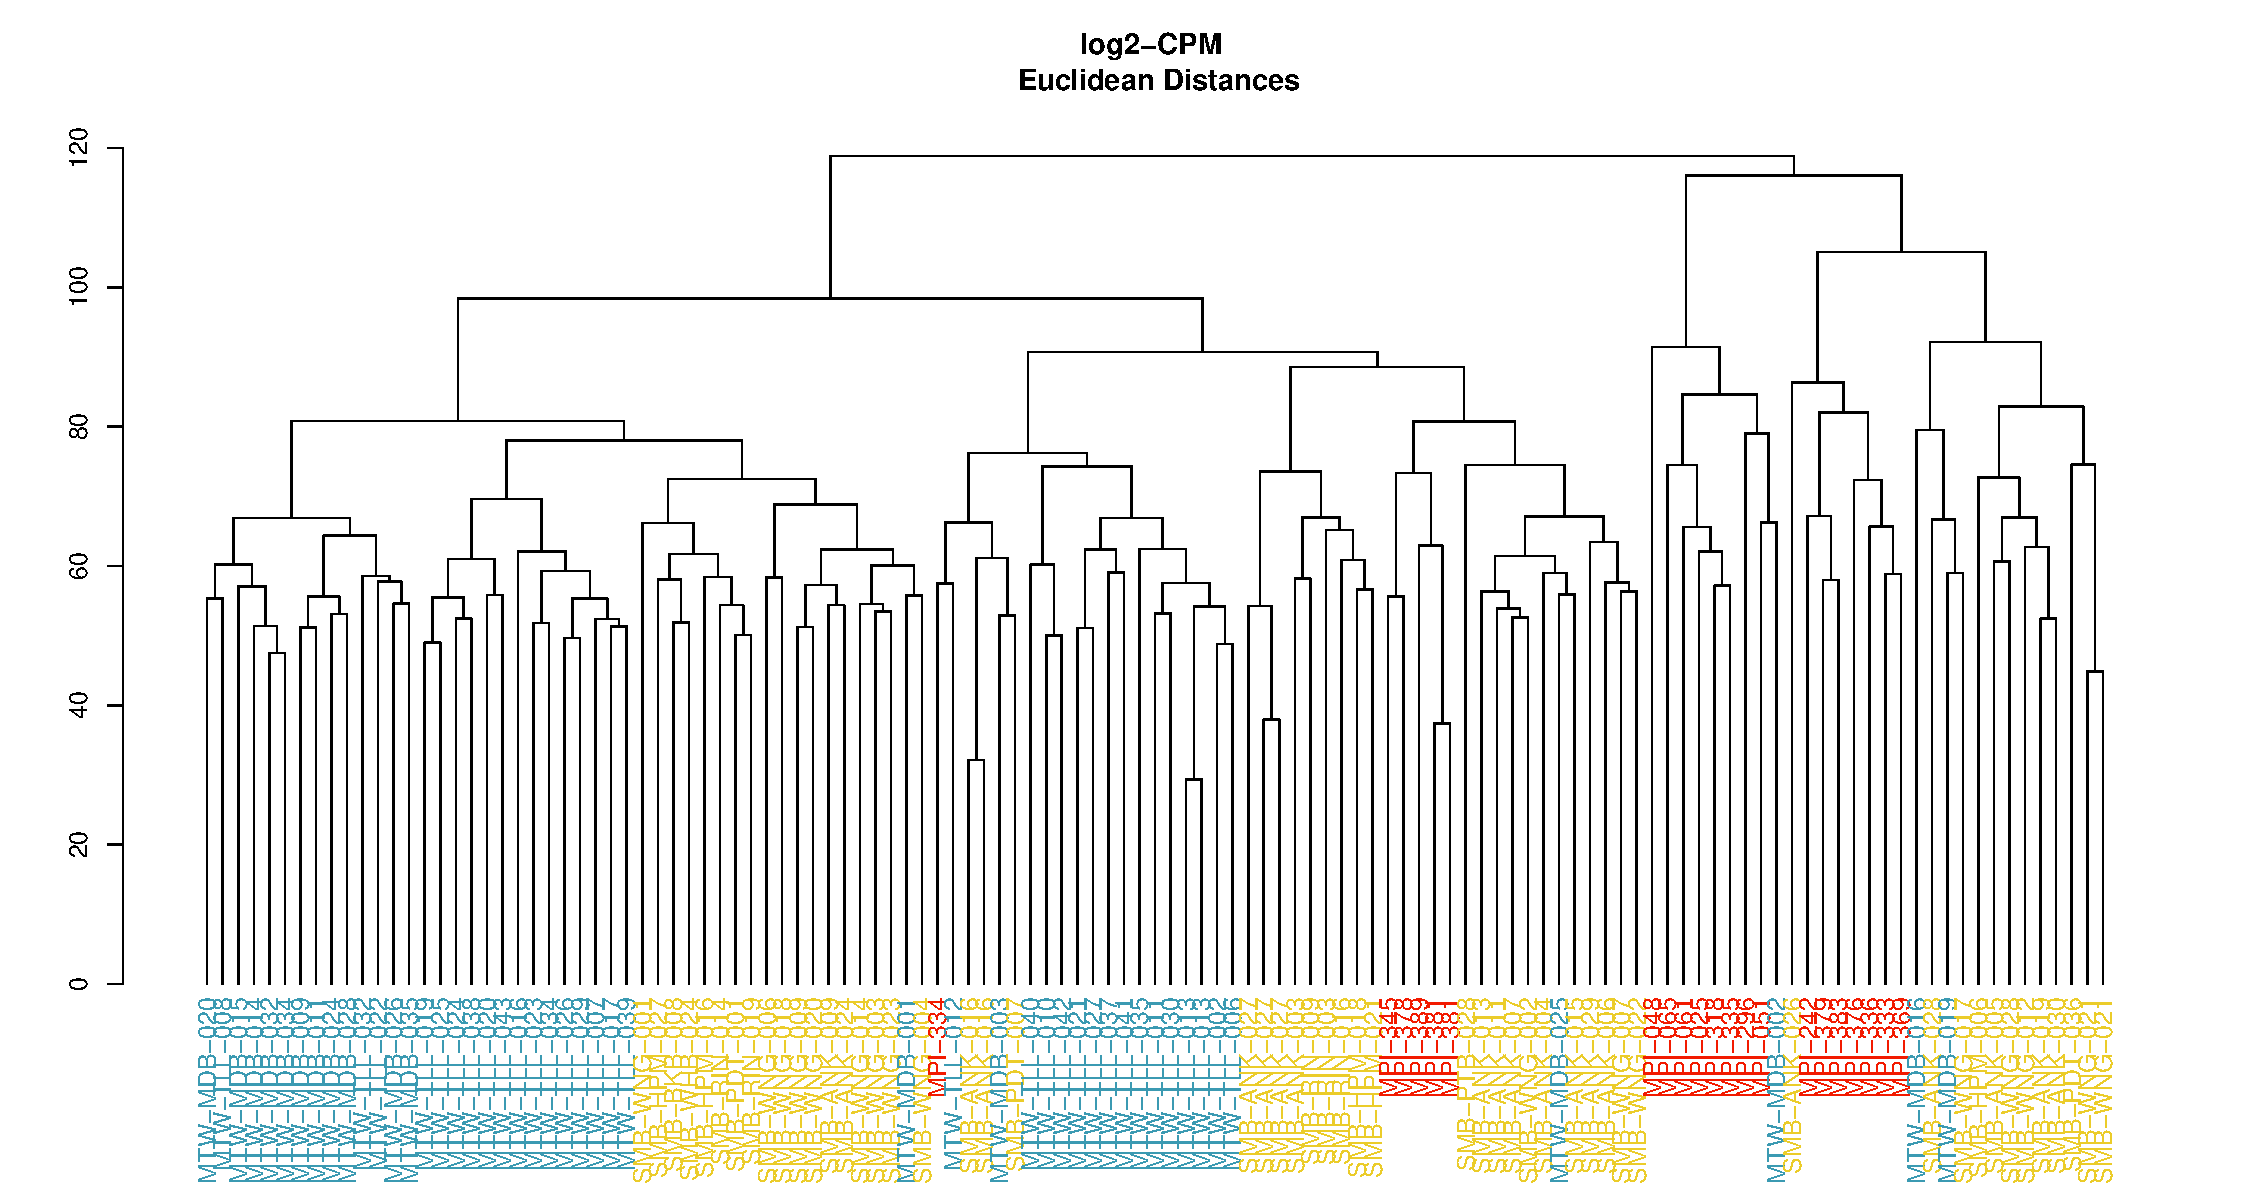
\includegraphics[width=\textwidth,height=\textheight,keepaspectratio]{Figures/SampleDistances_Euclidean.pdf}
\caption{Hierarchical clustering of log2-transformed CPM values of TMM- normalised counts. Yellow indicates samples from Sumba, red indicates samples from Mappi, and blue indicates samples from Mentawai. Clustering can be seen predominantly by island.}
\label{fig:Euclidean Sample Distances}
\end{figure}

\begin{figure}[htb!]
\centering
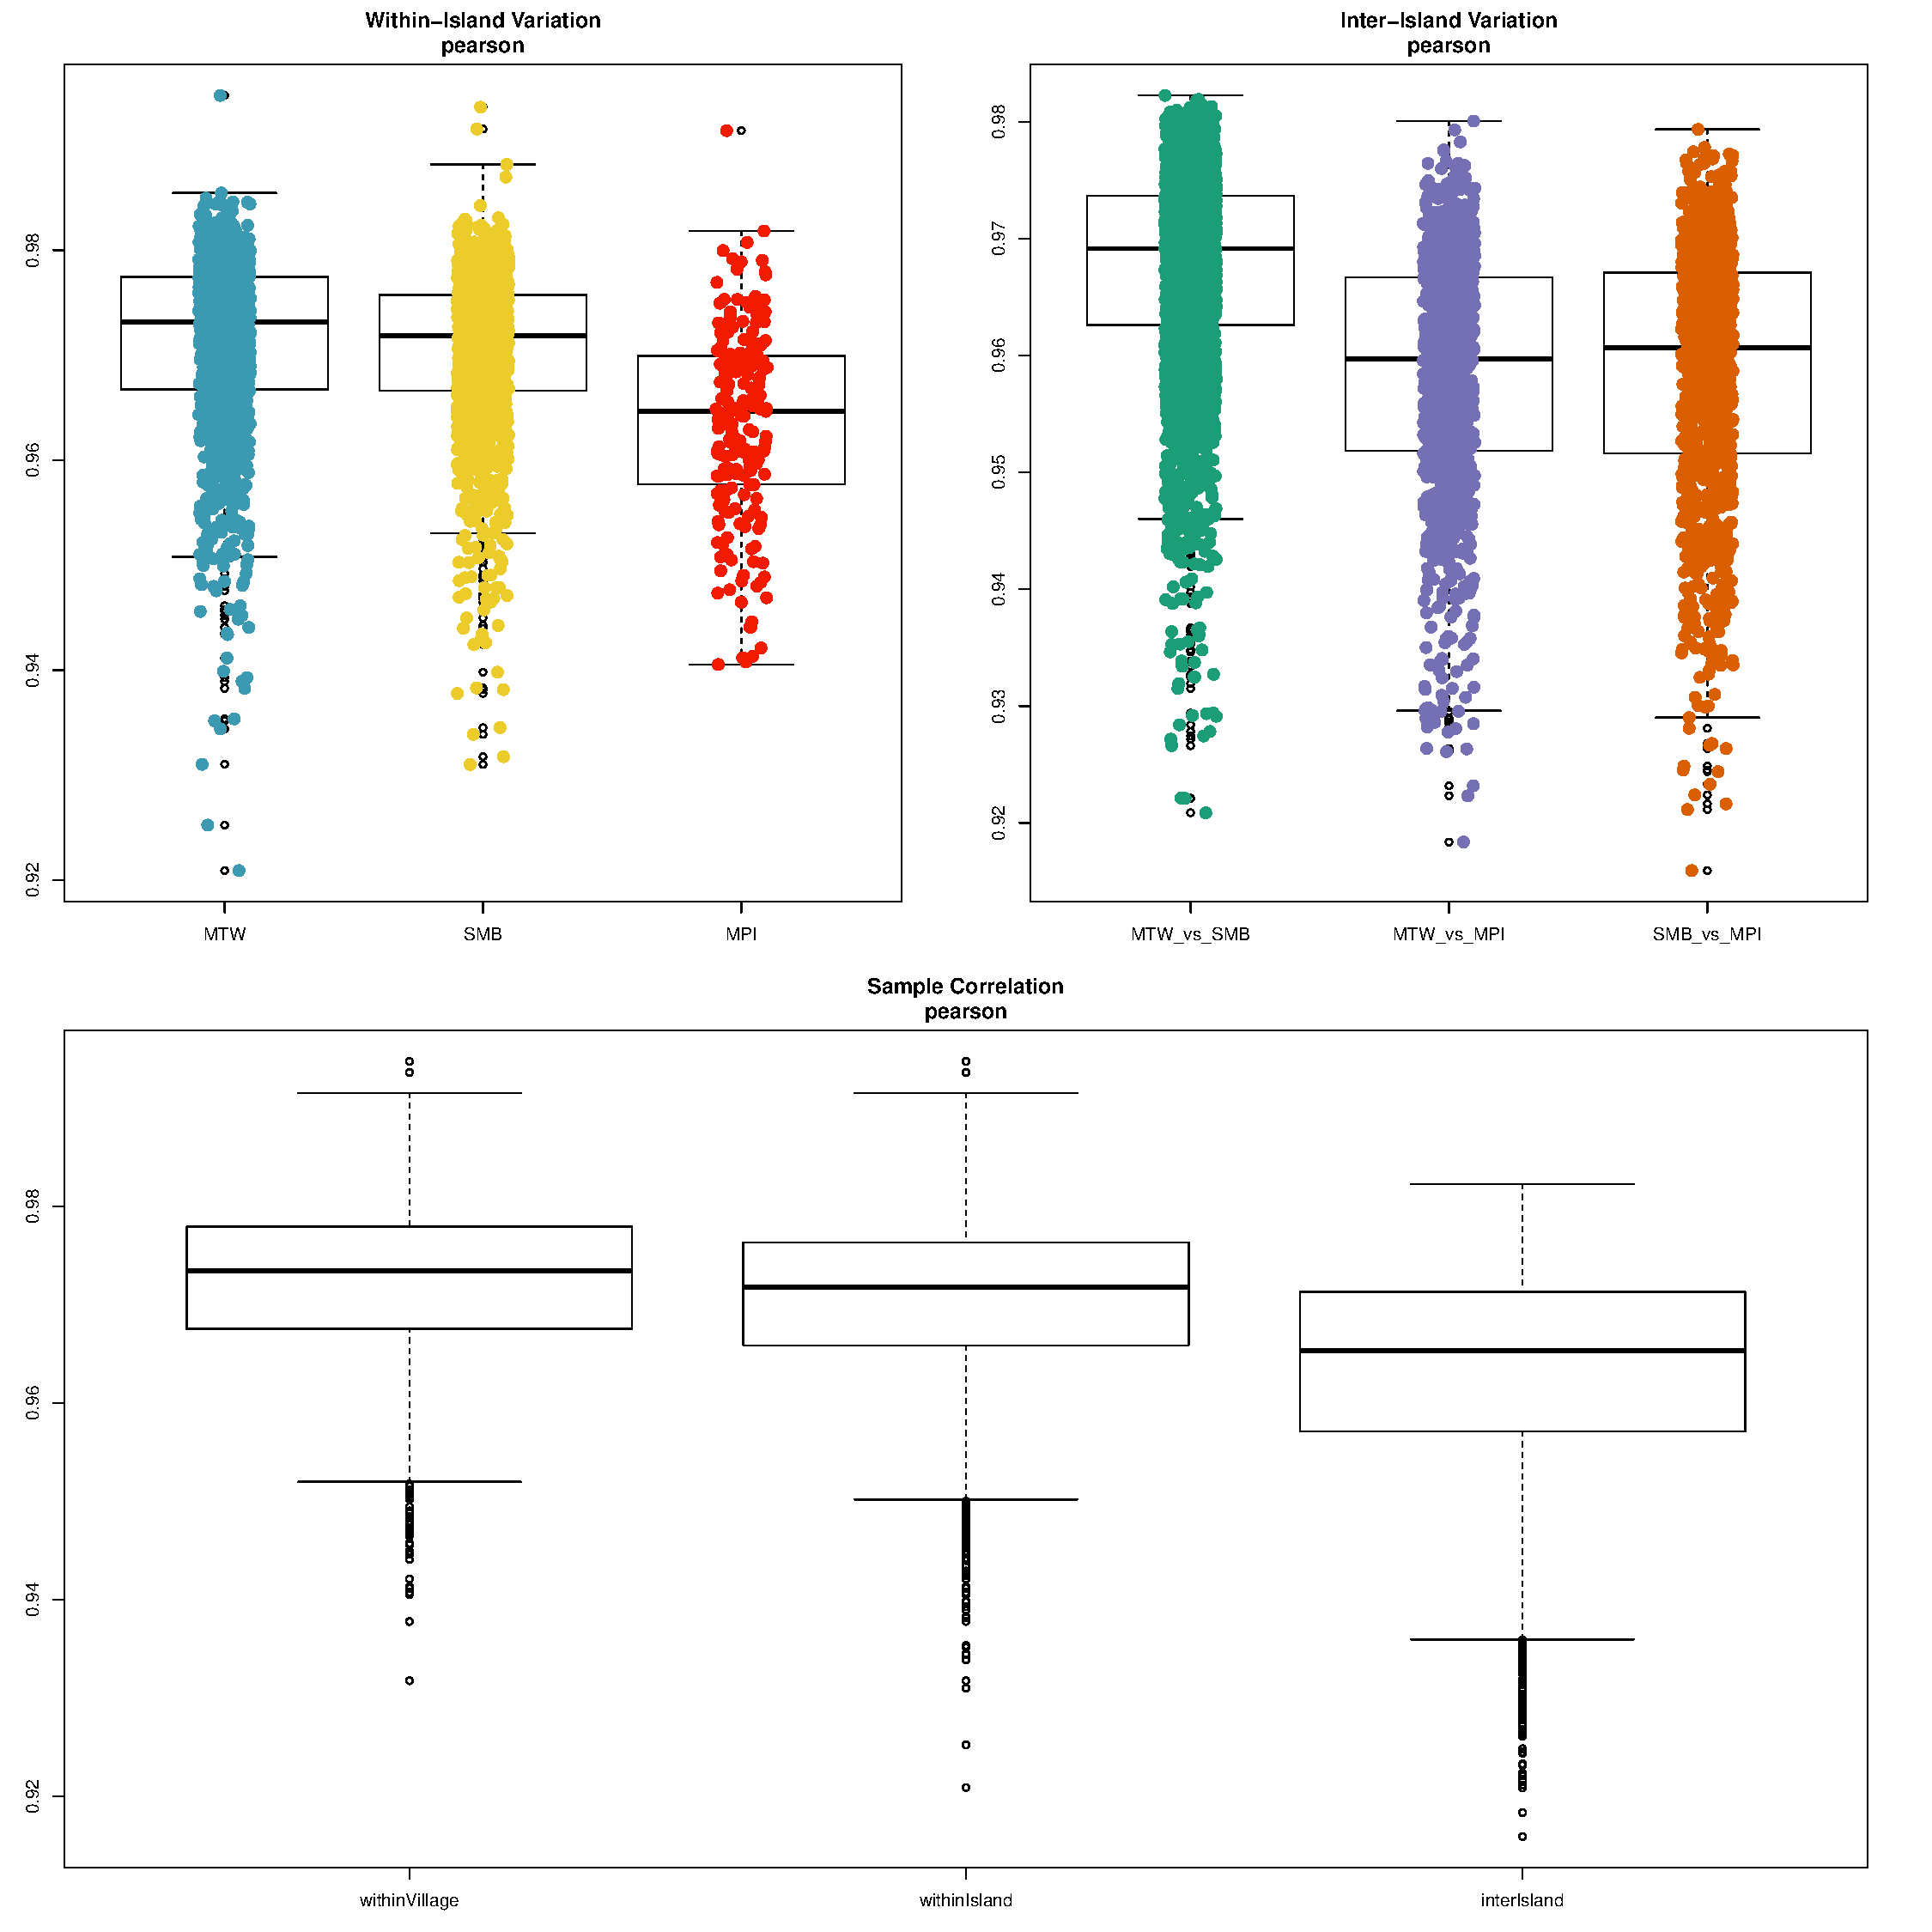
\includegraphics[width=\textwidth,height=\textheight,keepaspectratio]{Figures/IslandVariation_pearson.pdf}
\caption{Within and between island variation in all three island populations using Pearson correlations of the log2-transformed, TMM-normalised CPM values.}
\label{fig:Island Variation}
\end{figure}

\section{Differential expression analysis}
Because clear clustering was observed by batch, age, RIN score, and blood type (CD8T, CD4T, NK, B cells, monocytes, and granulocytes), I incorporated these known covariates into the design matrix of my linear model. The final model used to test for differential expression was therefore:

\textbf{\textit{~0 + Island + Age + batch + RIN + CD8T + CD4T + NK + Bcell + Mono + Gran}}

where island is the covariate of interest and Age, batch, RIN, and blood types are the covariates affecting expression levels. I then set up a list of contrasts comparing each island population, which consisted of the following contrasts: Sumba versus Mentawai, Sumba versus Mappi, and Mentawai versus Mappi.  
I removed high sample variability from the count data using Voom-normalisation on the TMM-normalised sample counts. Voom estimates the mean-variance relationship of log2 CPM-normalised counts and generates a precision weight for each sample (cite). This approach enables poor-quality samples to be down-weighted and effectively eliminates the mean-variance relationship (Figure \ref{fig:Voom normalisation}). Since technical replicates were used in the study design, the limma function duplicateCorrelation was used in order to estimate the correlation between expression measurements made on the same subject (cite limma manual). DuplicateCorrelation takes information from replicated samples and uses an empirical Bayes method to moderate the standard deviation between genes (cite limma manual). After running duplicateCorrelation on the samples, I then ran Voom a second time to incorporate the technical replicates as blocking variables and to feed in the estimated correlation within the blocks. A simple linear regression model was then fit to the voom output for each gene and an empirical Bayes moderated t-statistic was used to test each individual contrast from the design matrix equal to zero. When fitting the t models, I used the ‘robust’ parameter in Limma’s ‘eBayes’ function in order to deal with outlier genes that have abnormally high or low variance. I then identified significant genes using an adjusted p-value of 0.01 (Benjamini–Hochberg corrected; Benjaminini and Hochberg 1995) and an absolute log-fold change of 1. 

\begin{figure}[htb!]
\centering
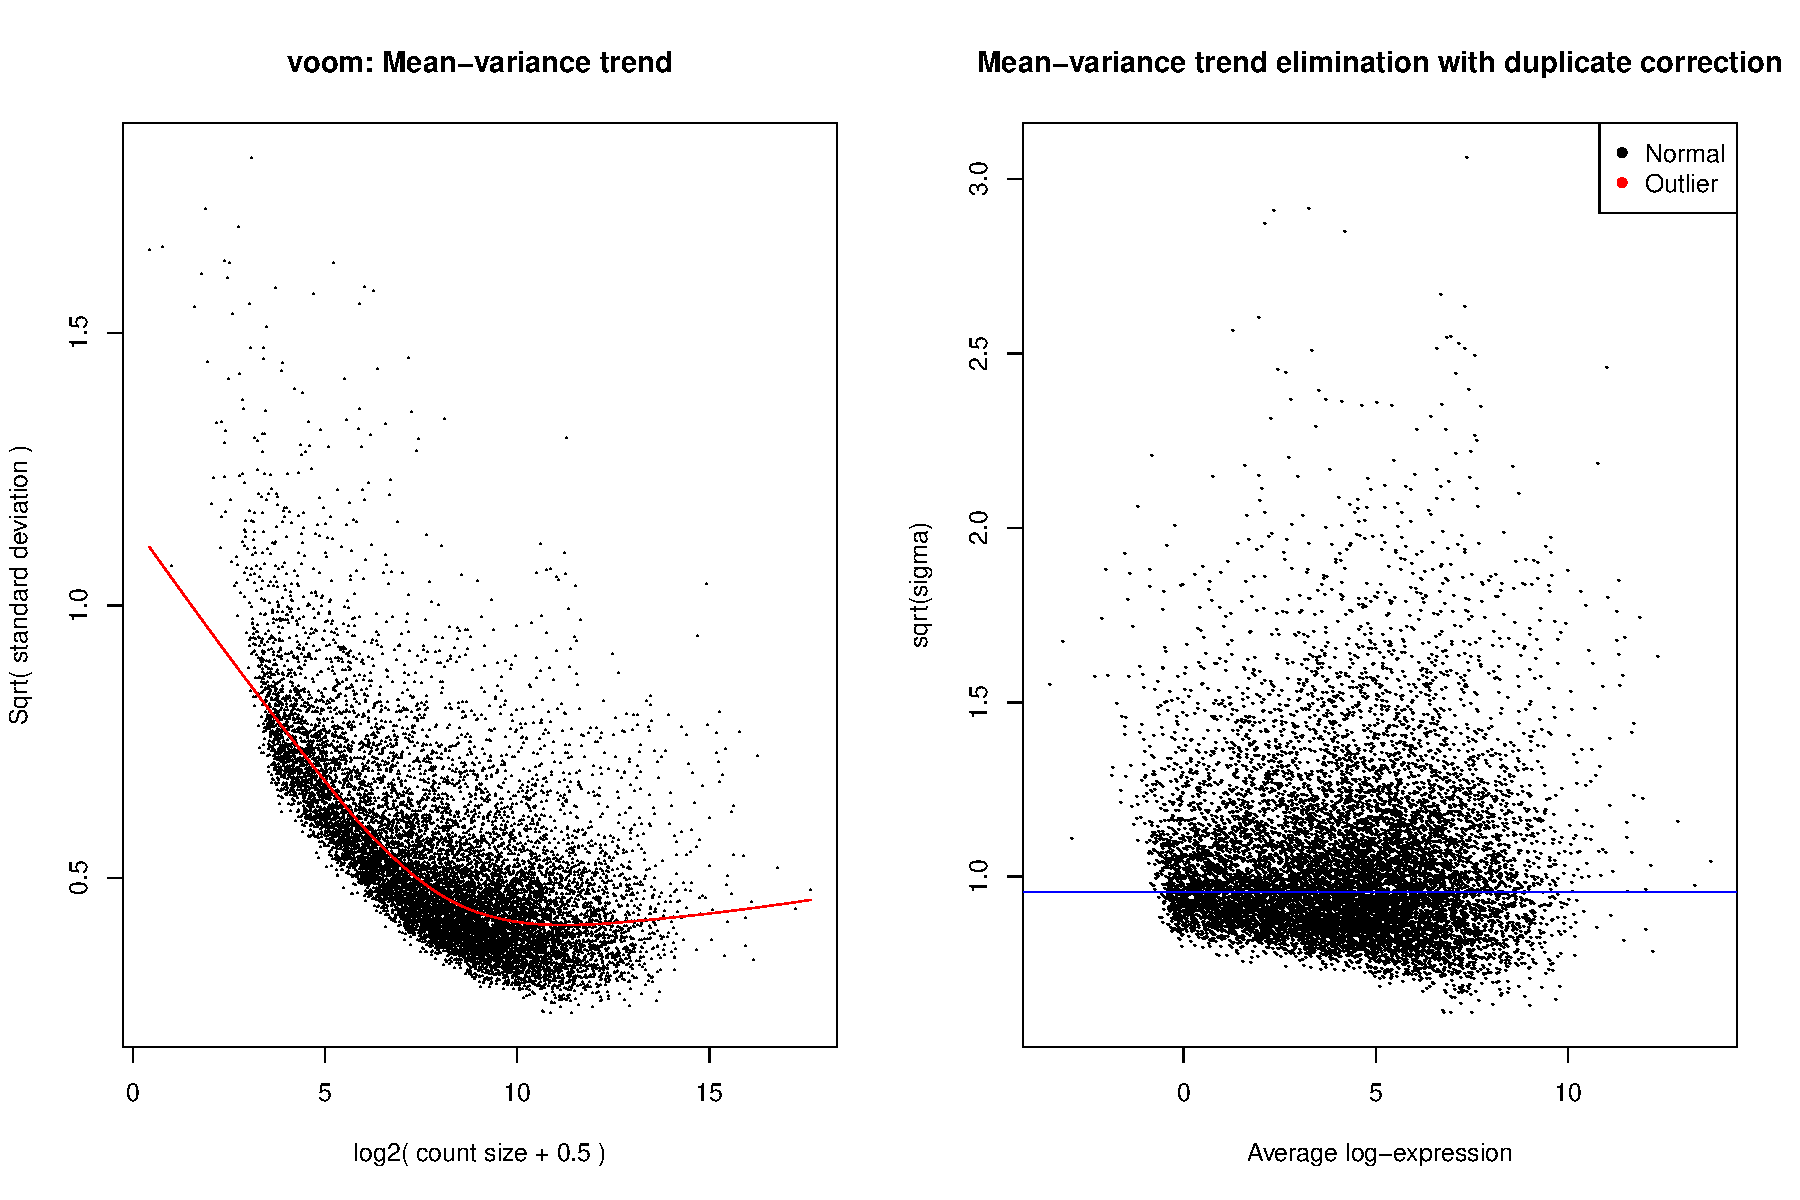
\includegraphics[width=\textwidth,height=\textheight,keepaspectratio]{Figures/Limma_voomDuplicateCorrelation_TMMNormalisation.pdf}
\caption{Mean-variance trend and elimination of the trend after applying Voom-normalisation to the TMM-normalised count data.}
\label{fig:Voom normalisation}
\end{figure}

\section{RUVs}
In addition to removing batch effects by regressing out known variables affecting gene expression, I also tested an alternative unsupervised batch-correction method using RUV (cite). RUV uses factor analysis to control for technical effects based on control genes or samples. For this analysis, I chose RUVs which utilizes counts of negative control samples. Unlike RUVg which uses control genes to correct for technical effects, RUVs is less sensitive to the control genes used in the factor analysis. Because of this and the availability of technical replicates, RUVs was chosen as the RUV correction method. 
The first step of RUVs is to set up a count matrix using raw read counts. I did this using all raw reads filtered for lowly-expressed genes. I then performed upperquartile normalization on the dataset and checked the performance before and after correction (Figure \ref{fig:UQ normalisation}). 

\begin{figure}[htb!]
\centering
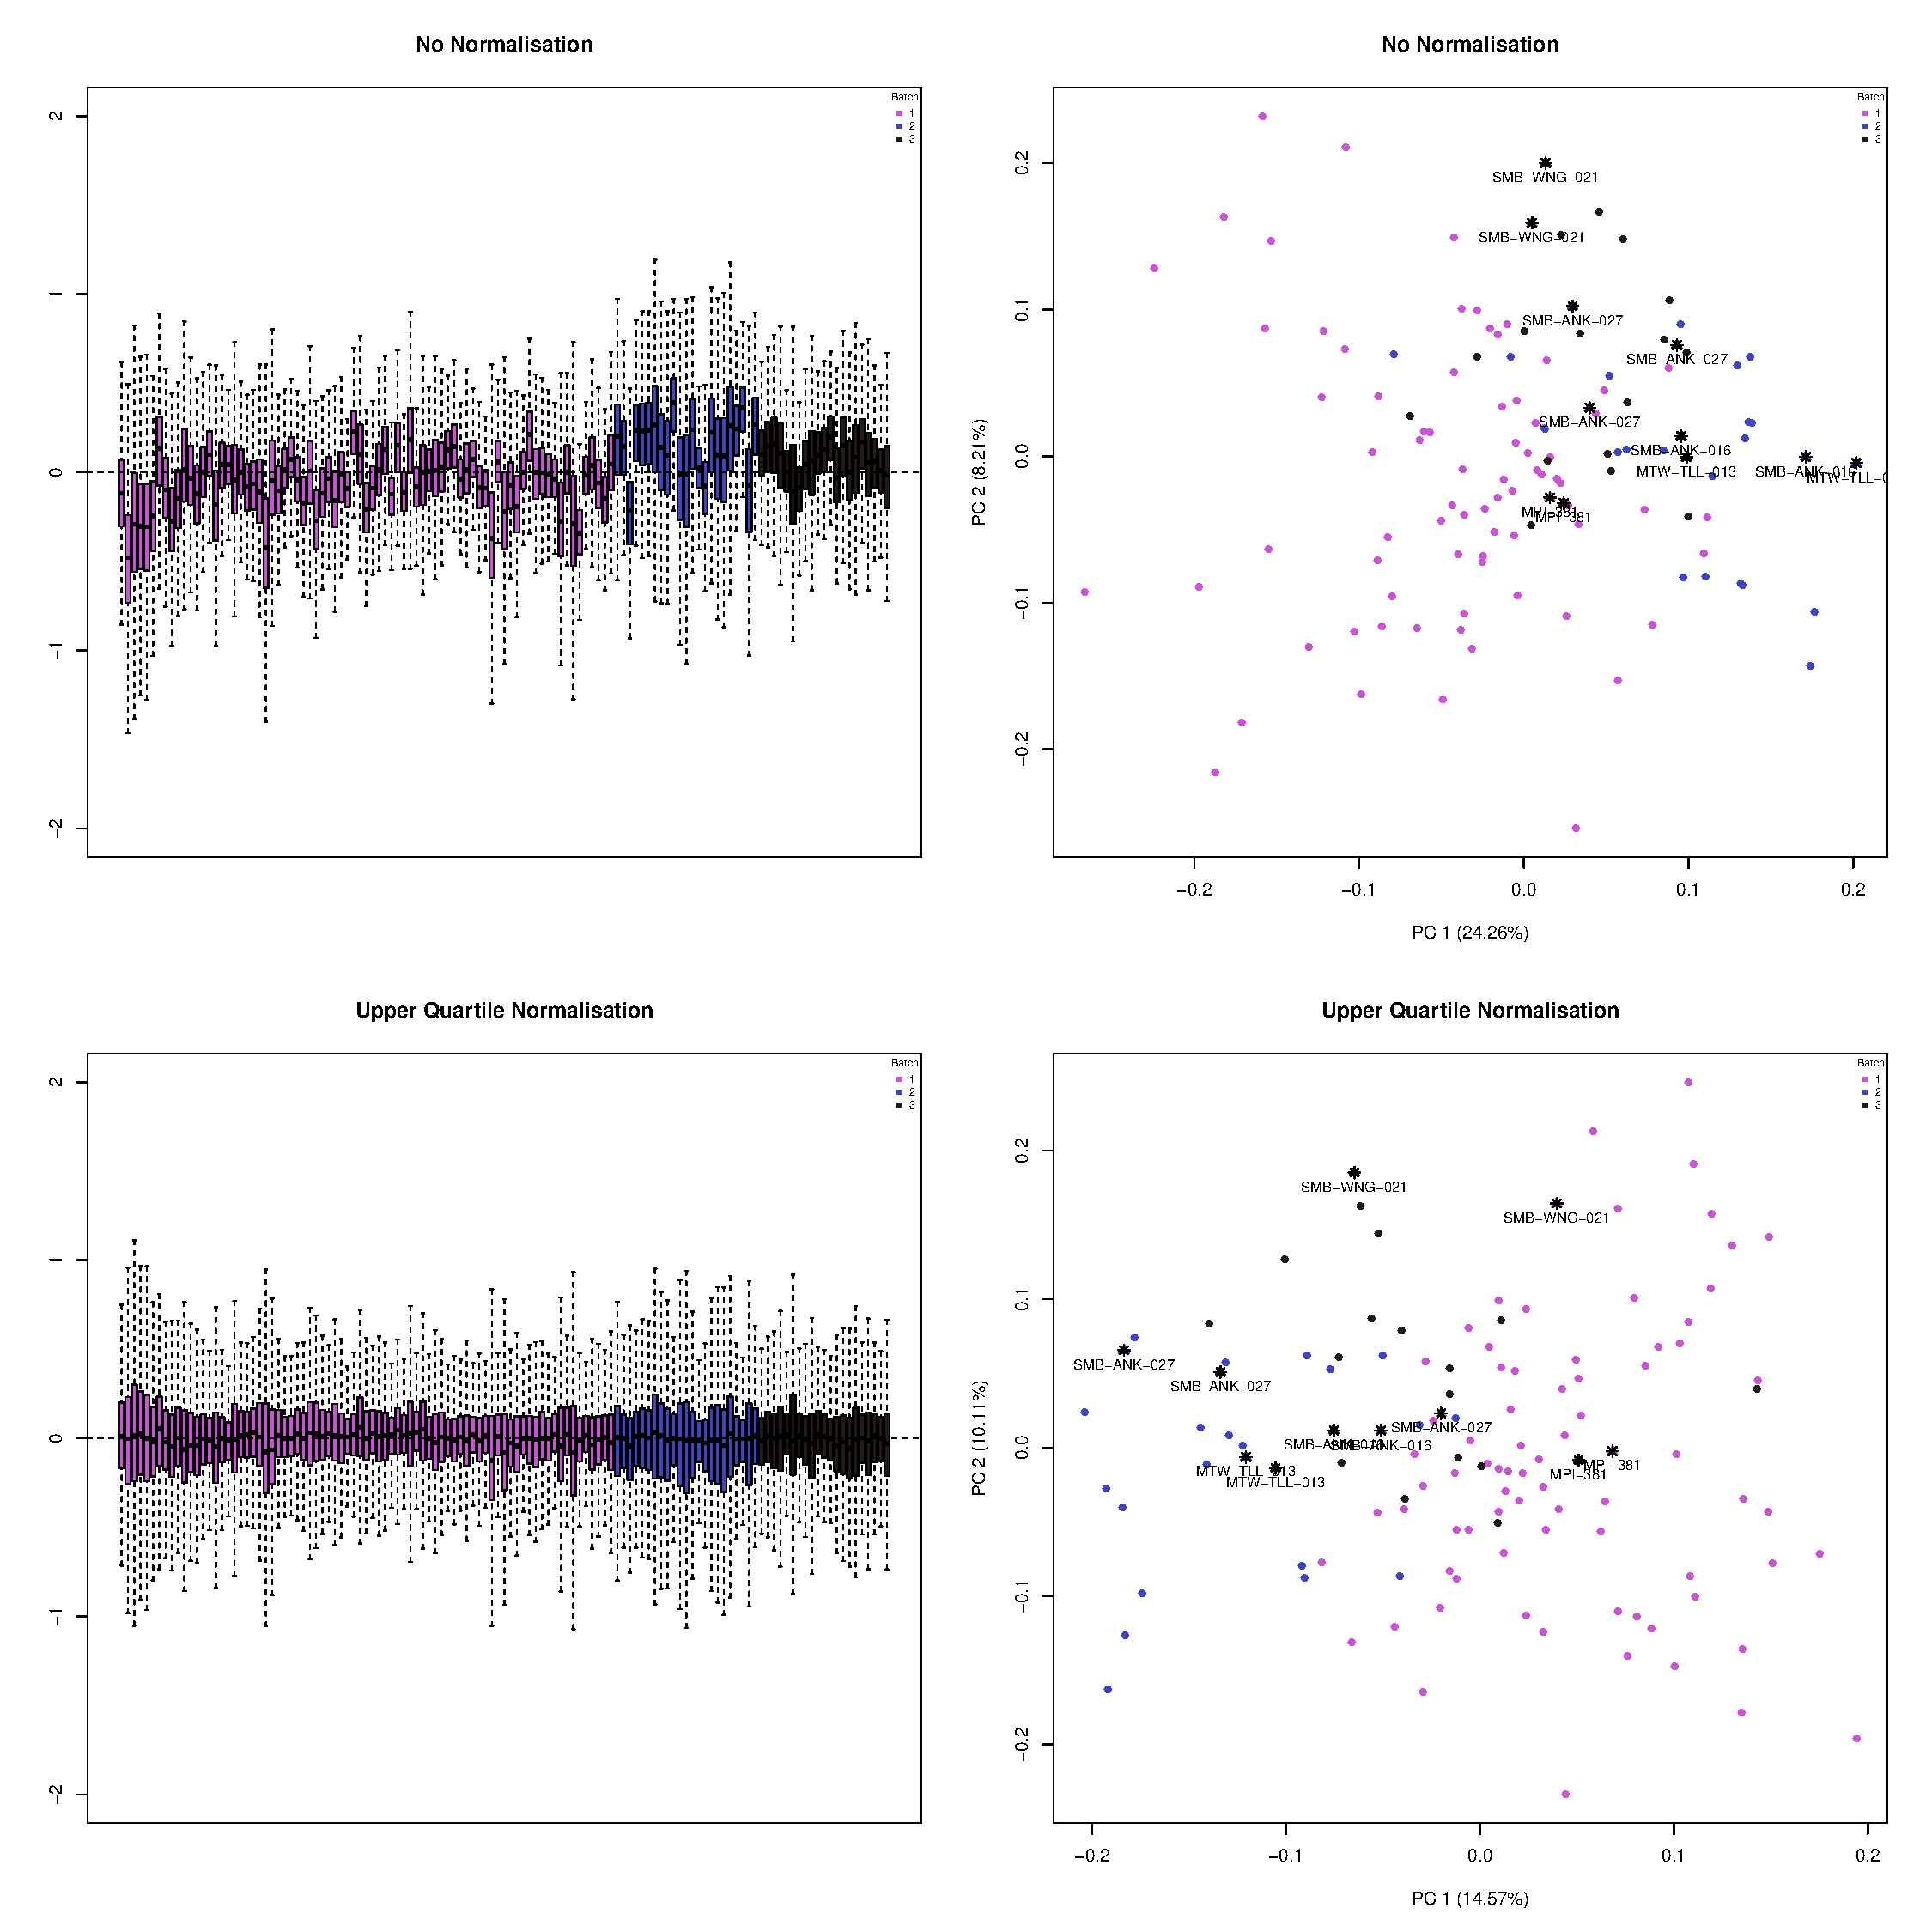
\includegraphics[width=\textwidth,height=\textheight,keepaspectratio]{Figures/Normalisation_beforeandAfterUQnorm.pdf}
\caption{Sample variability of raw read counts before and after upperquartile normalisation. An RLE plot showing the total amount of variability in each batch (batch 1=pink,batch 2=purple, batch 3=black) can be seen before and after upperquartile normalisation (top and bottom left, respectively). Principal component analysis of the first two PCs before and after upperquartile normalisation (top and bottom right,respectively) are shown to cluster by batch. Sample replicates are highlighted with stars.}
\label{fig:UQ normalisation}
\end{figure}

In order to perform RUVs on the raw read counts, RUVs needs four pieces of information: 1) the object containing read counts, 2) a list of control genes, 3) k, the model parameter indicating the number of hidden factors of variation, and 4) replicate information. For the object containing read counts, I used the upperquartile-normalised reads filtered for lowly-expressed genes. I then used all genes within the dataset for control genes, as this has been shown to perform well in an RUVs pipeline (cite). For k, the number of hidden factors of variation, I tested values from one to six (the highest value of k is the total number of replicates in the study) and analysed the total amount of variation through RLE and PCA plots (Figure \ref{fig:K Performance}). A k of three to six was most effective in reducing the total amount of variation (Figure \ref{fig:K Performance}, panels e, g, i, and k) and minimizing distances between technical replicates (Figure \ref{fig:K Performance}, panels f, h, j, and l). In addition to looking at total variation, I also plotted the p-value distribution and total number of differentially expressed genes at an FDR of 0.01 and log fold change of 1 (Figure \ref{fig:DE Genes K}). For each population comparison, I chose the best value of k as the inflection point in the total number of differentially expressed genes. This changed for each population comparison (Sumba vs Mentawai = 4, Sumba vs Mappi = 5, Mentawai vs Mappi = 3) and therefore chose a k of 5 based on its performance in the PCA and RLE plots. 

\begin{figure}[htb!]
\centering
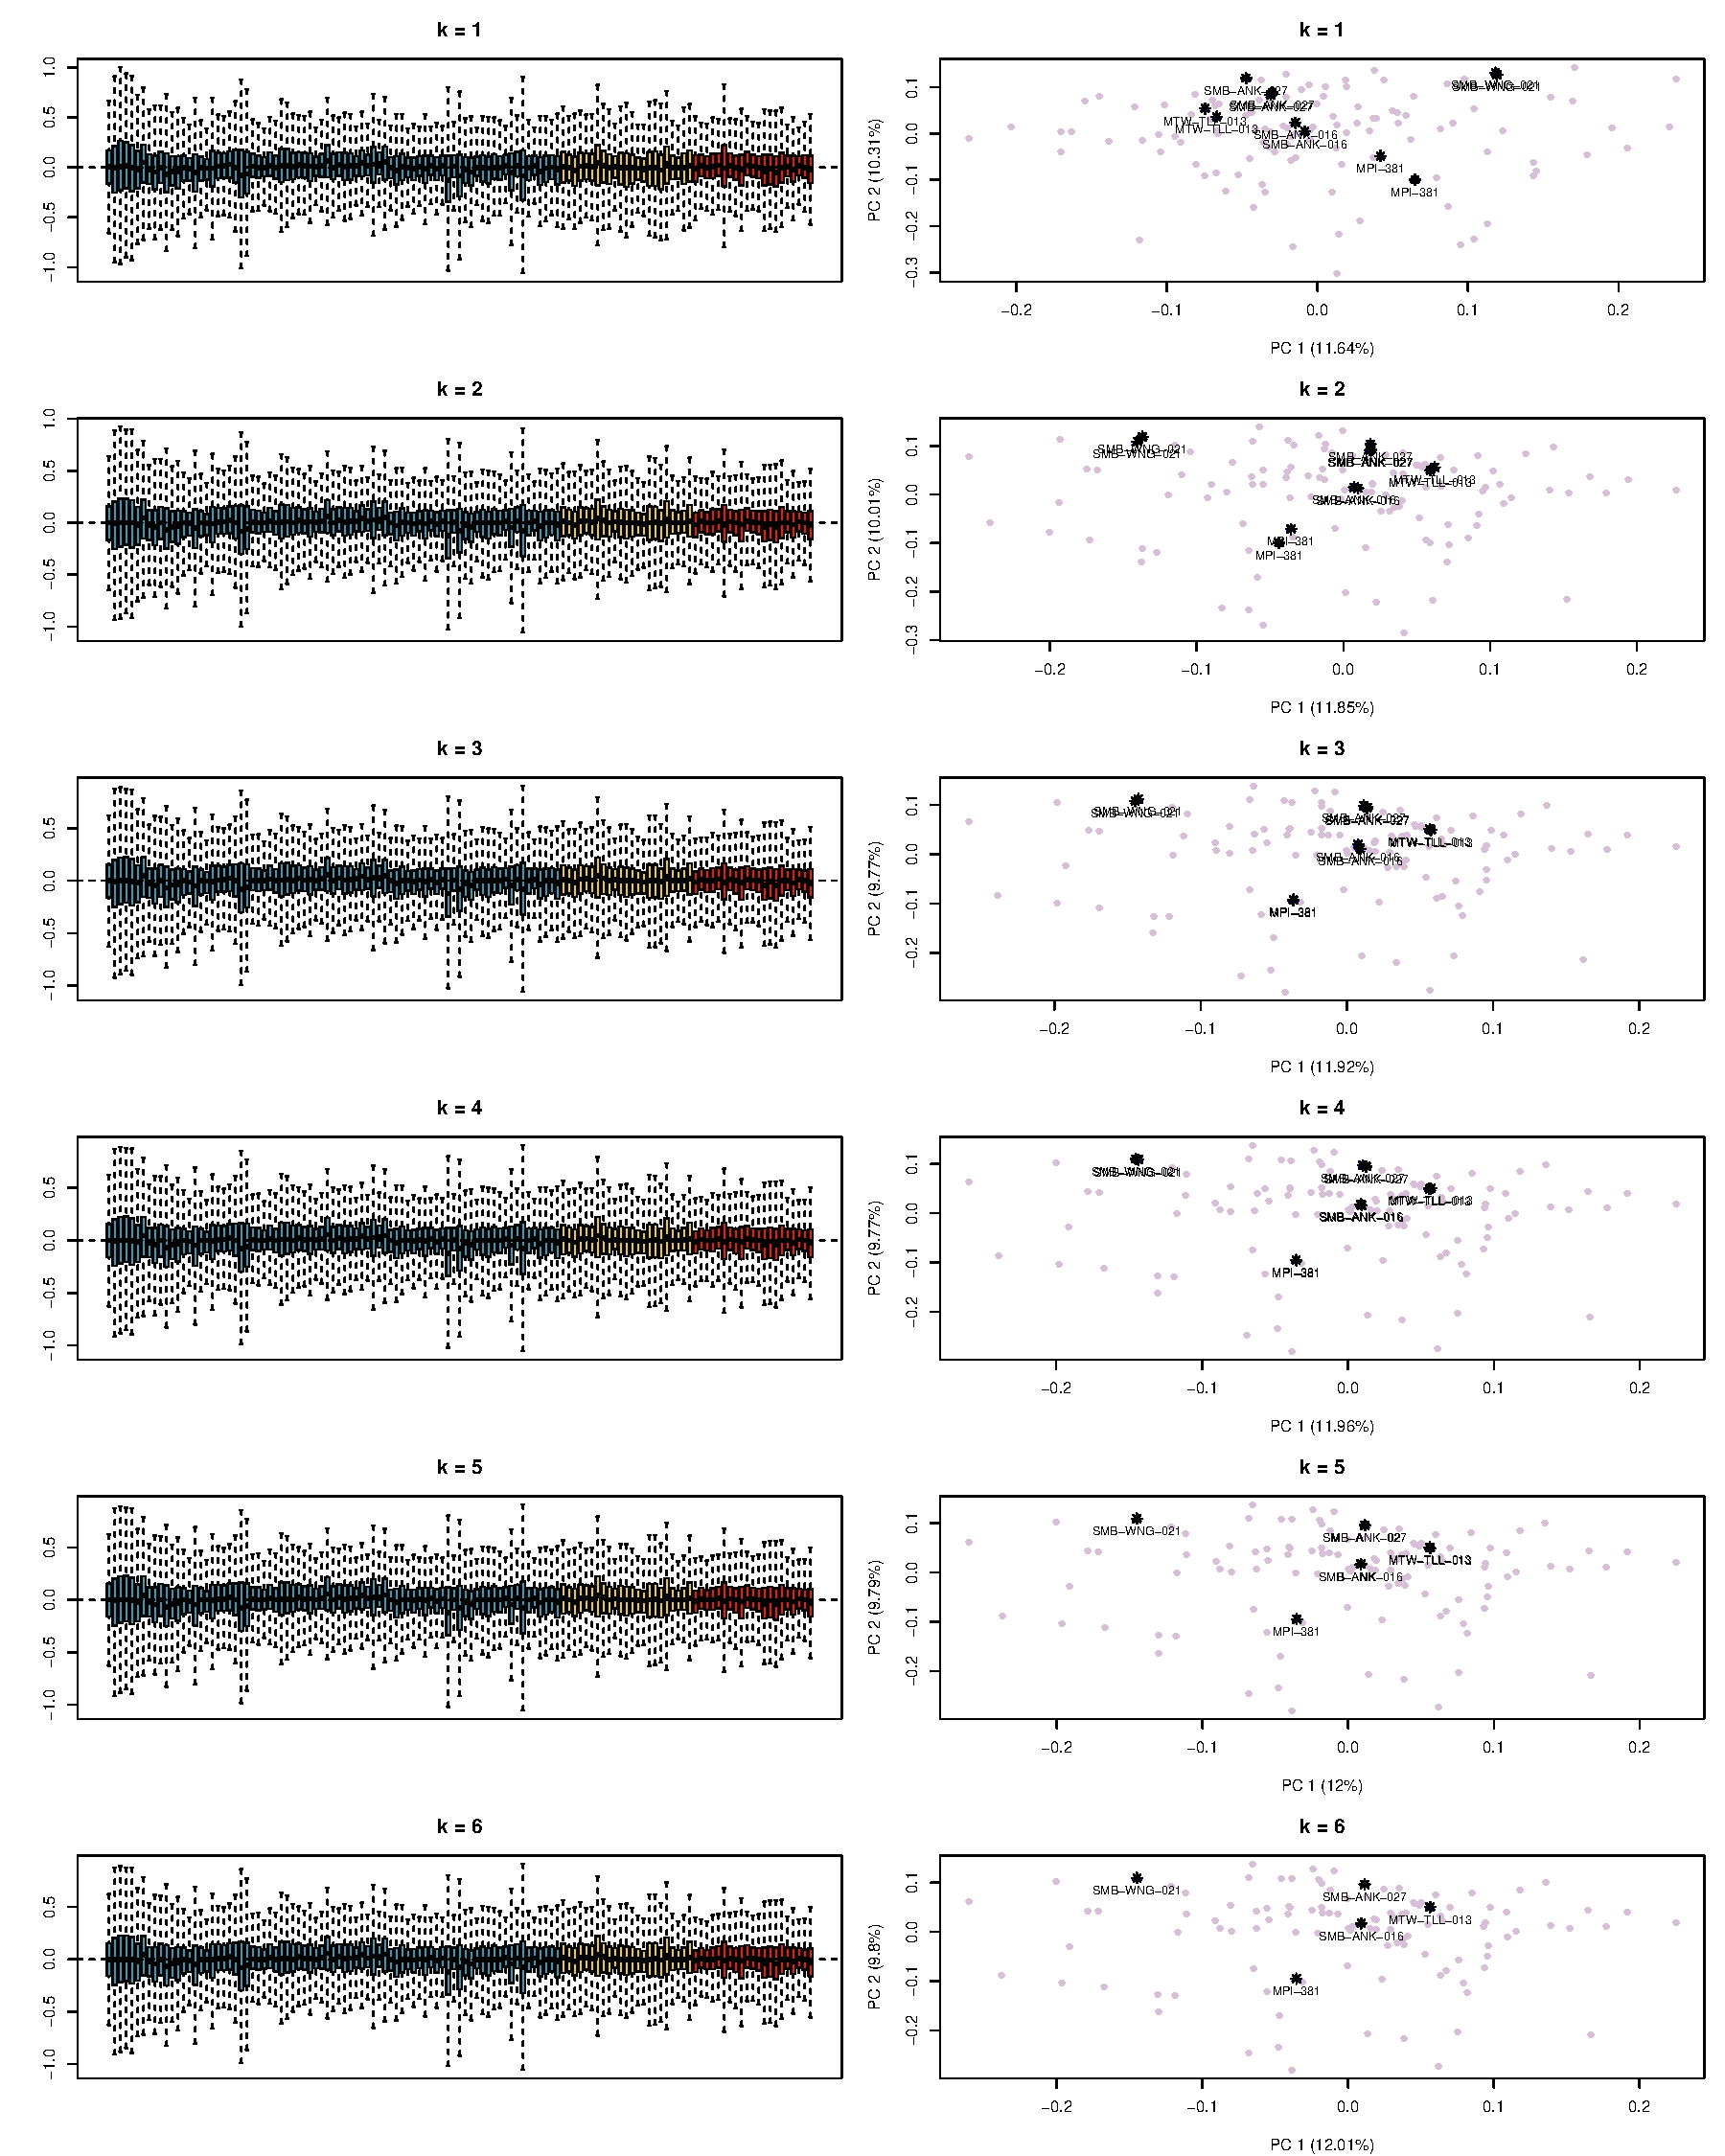
\includegraphics[width=\textwidth,height=\textheight,keepaspectratio]{Figures/RUVsNormalisation_choosingK.pdf}
\caption{Performance of varying levels of k. Left: RLE plots highlighted by island show the amount of variability for varying levels of k. Right: Principal component analysis of the first two dimensions can be seen for a k of one to six. A k of three and higher results in reduced variability as well as technical replicates sitting closer together.}
\label{fig:K Performance}
\end{figure}

\begin{figure}[htb!]
\centering
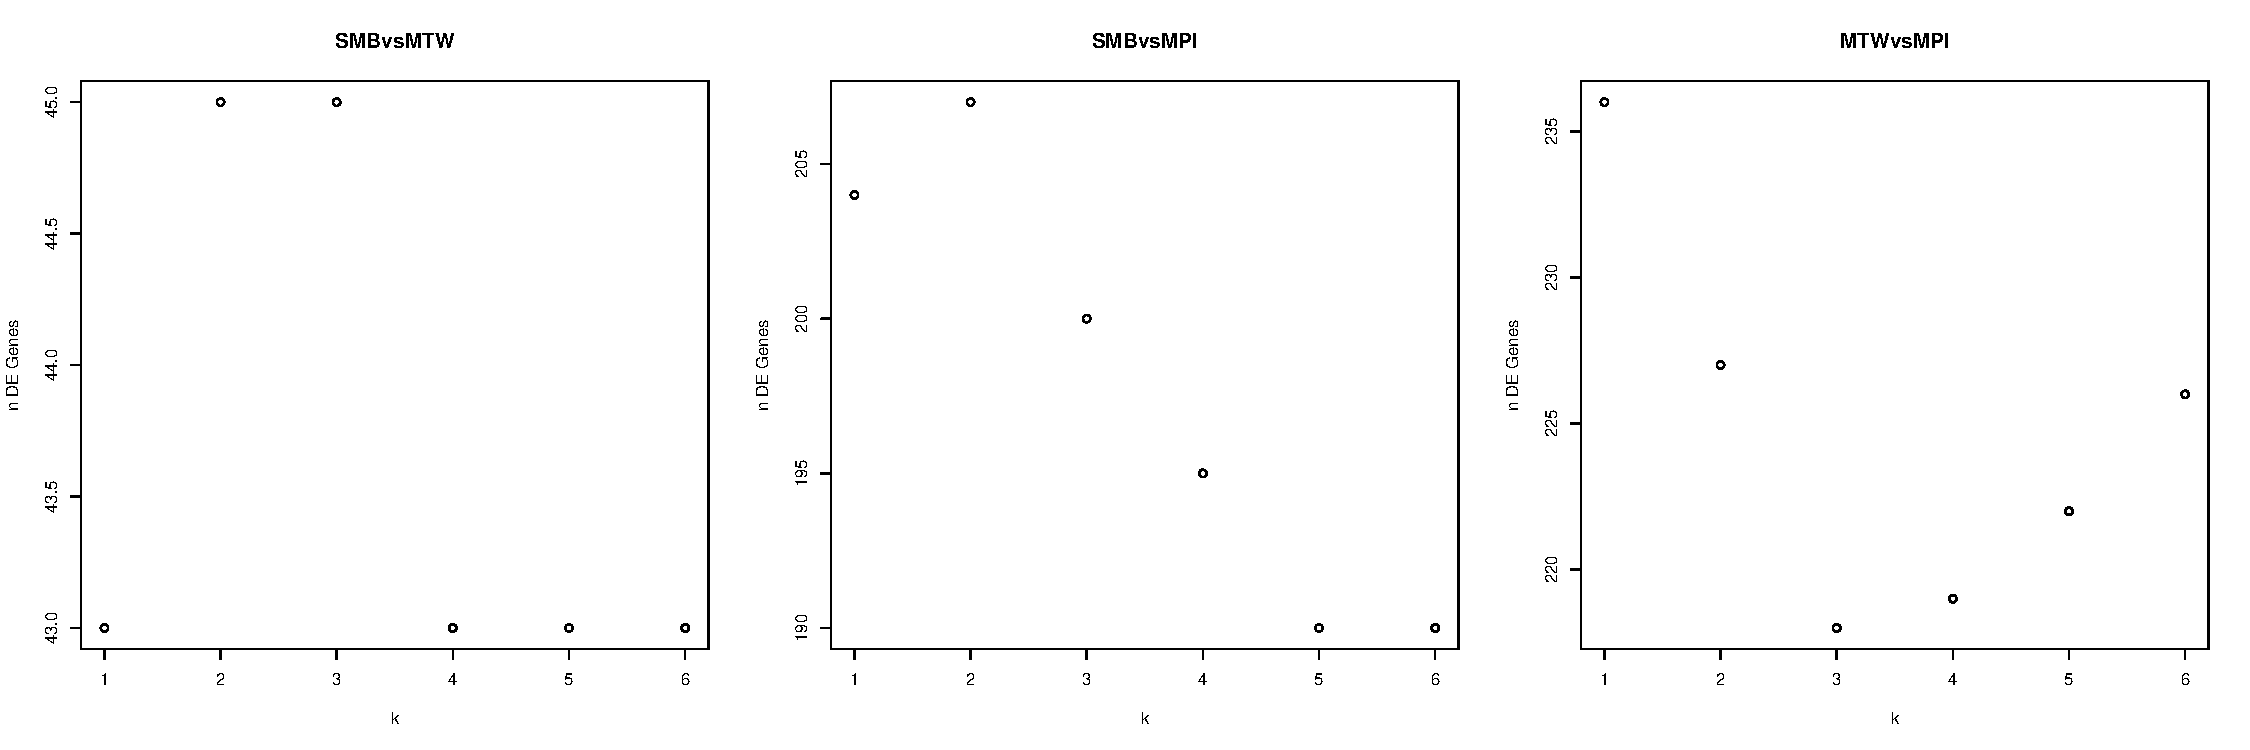
\includegraphics[width=\textwidth,height=\textheight,keepaspectratio]{Figures/numberDeGenes_choosingK_RUVs.pdf}
\caption{Total number of differentially expressed genes for varying levels of k. The significance threshold was set to an FDR of 0.01 and a log fold change of one. The inflection point for the number of differentially expressed genes can be seen to vary for each population comparison.}
\label{fig:DE Genes K}
\end{figure}

RUVs outputs estimated factors of unwanted variation and normalised counts, which are obtained by regressing out the original counts on the unwanted factors. After obtaining the factors of unwanted variation from RUV, I used the same negative binomial GLM approach, as done in the Limma pipeline, using known covariates. In my model, I included my covariate of interest as island and the estimated values of k from all 5 hidden factors of unwanted variation (Supplementary Table 5). I then converted my RUVs-corrected dataset to a DGE-list object, normalised the data with upperquartile normalisation, and applied Voom to eliminate the mean-variance trend (Figure 1\ref{fig:Voom normalisation RUV}). As in the pipeline using known covariates (above), the duplicateCorrelation function was used was used in order to estimate the correlation between expression measurements made on the same subject, then Voom was run a second time to incorporate the technical replicates as blocking variables. The 'robust' parameter was used using Limma's eBayes function and all significant genes were identified using an adjusted p-value of 0.01 (Benjamini–Hochberg corrected; Benjaminini and Hochberg 1995) and an absolute log-fold change of 1. 

\begin{figure}[htb!]
\centering
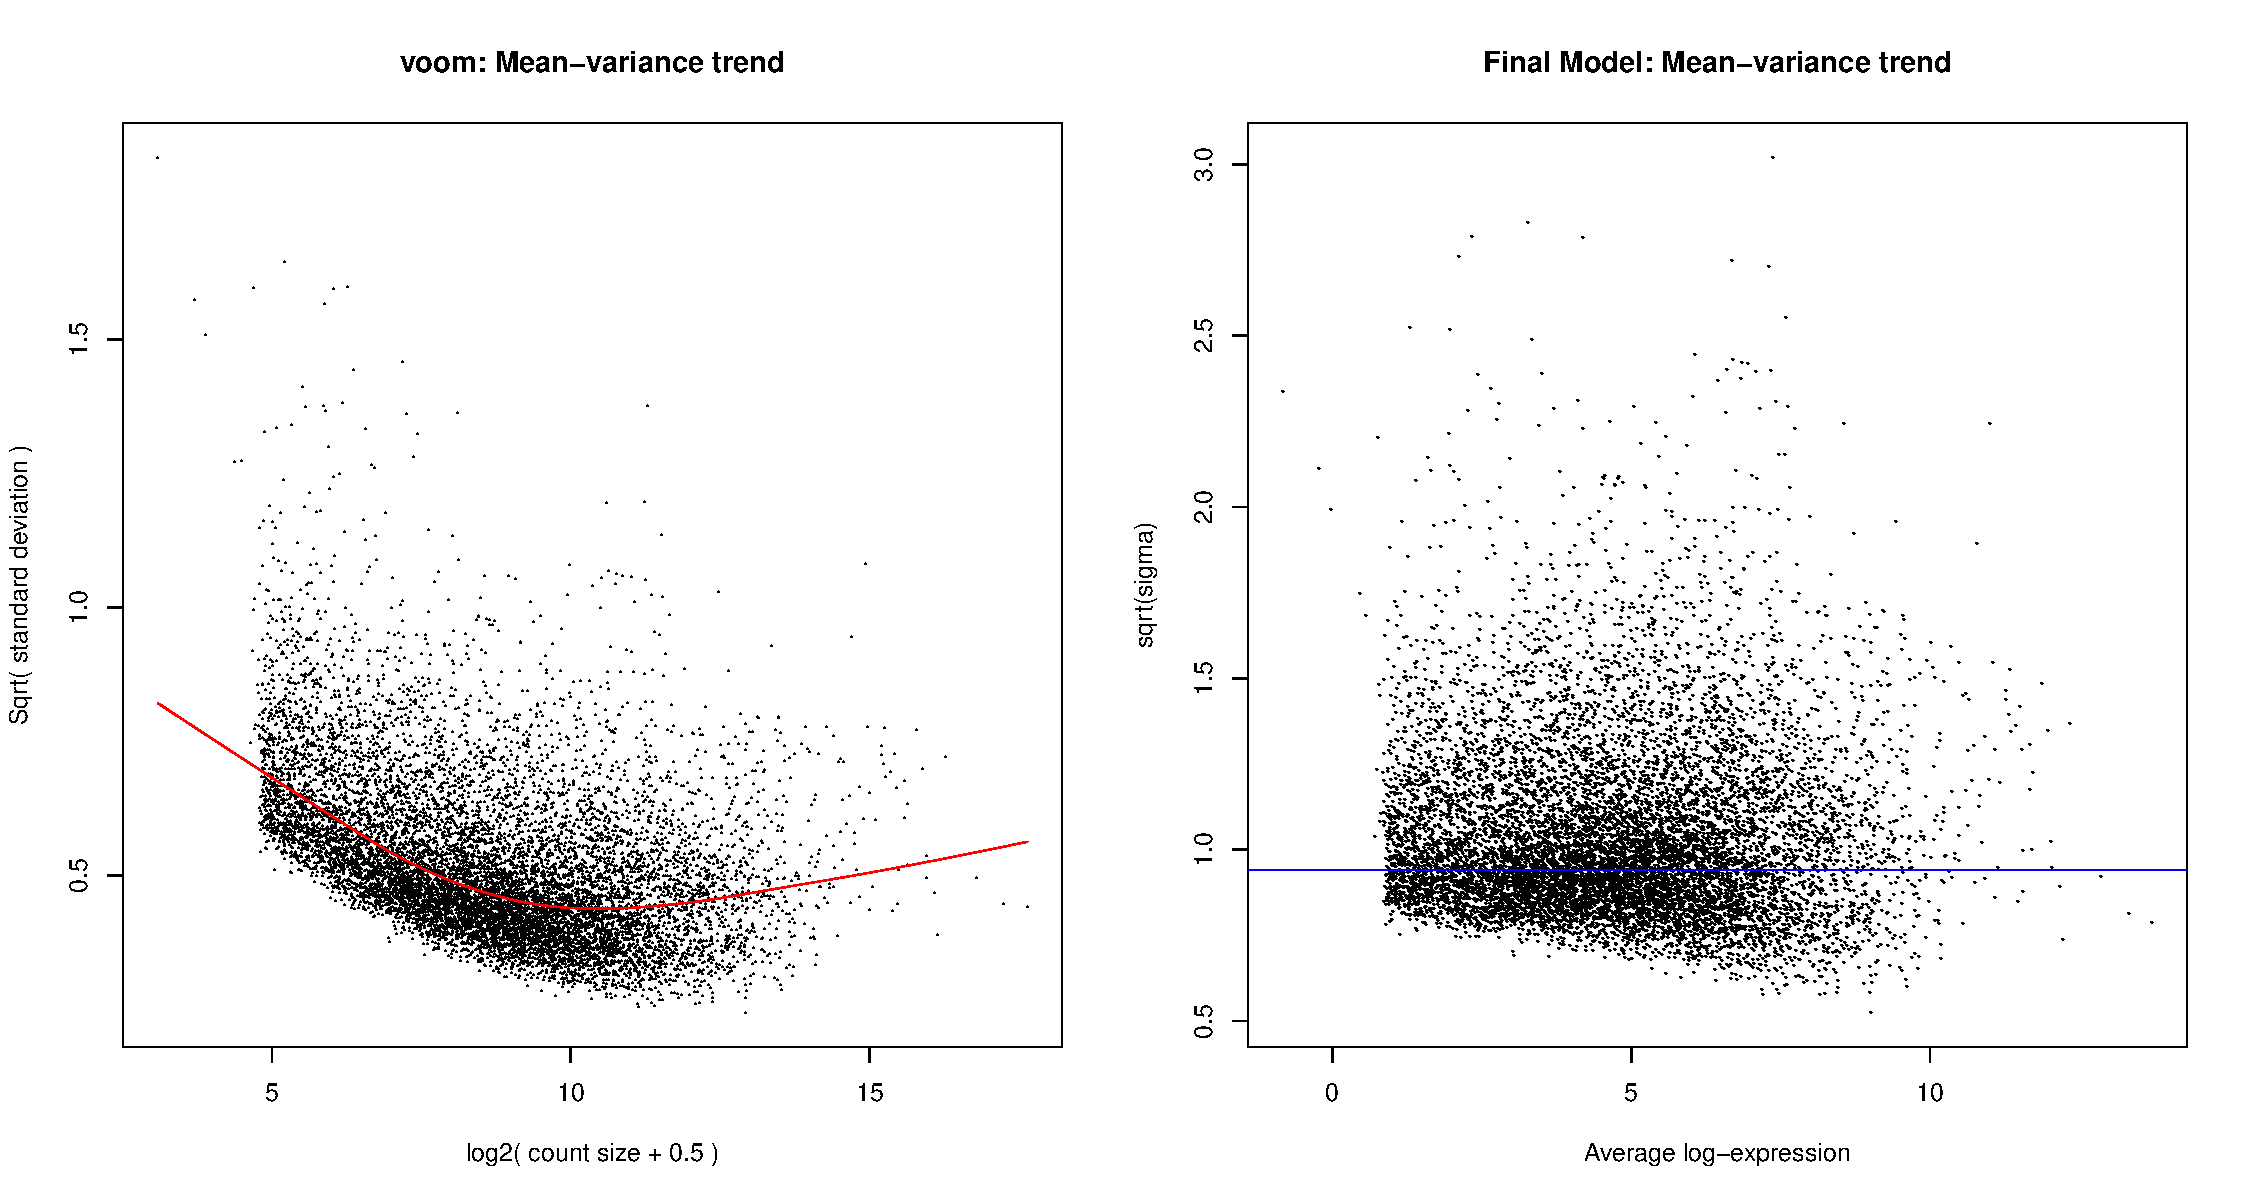
\includegraphics[width=\textwidth,height=\textheight,keepaspectratio]{Figures/Limma_voom_upperquartilenormalisation.pdf}
\caption{Mean-variance trend and elimination of the trend after applying Voom-normalisation to the upperquartile-normalised, RUVs-corrected count data.}
\label{fig:Voom normalisation RUV}
\end{figure}


\section{Comparing both}
After correcting for batch effects by regressing out known covariates influencing gene expression and with RUVs, I visually inspected grouping by batch through PCA analysis. The RUVs-corrected data had a higher percentage of variance in the first and second PCAs, whereas the limma-corrected data had less clustering by batch (Figure \ref{fig:RUV vs Limma: PCA by Batch}). Analysis of variance (ANOVA) between each dimension of the PCA and known covariates showed a stronger association between batch and the RUVs-corrected data than the limma-corrected data (Figure \ref{fig:RUV vs Limma: Heatmap of Covariates}, Supplementary Table 6, Supplementary Table 7). 

\begin{figure}[htb!]
\centering
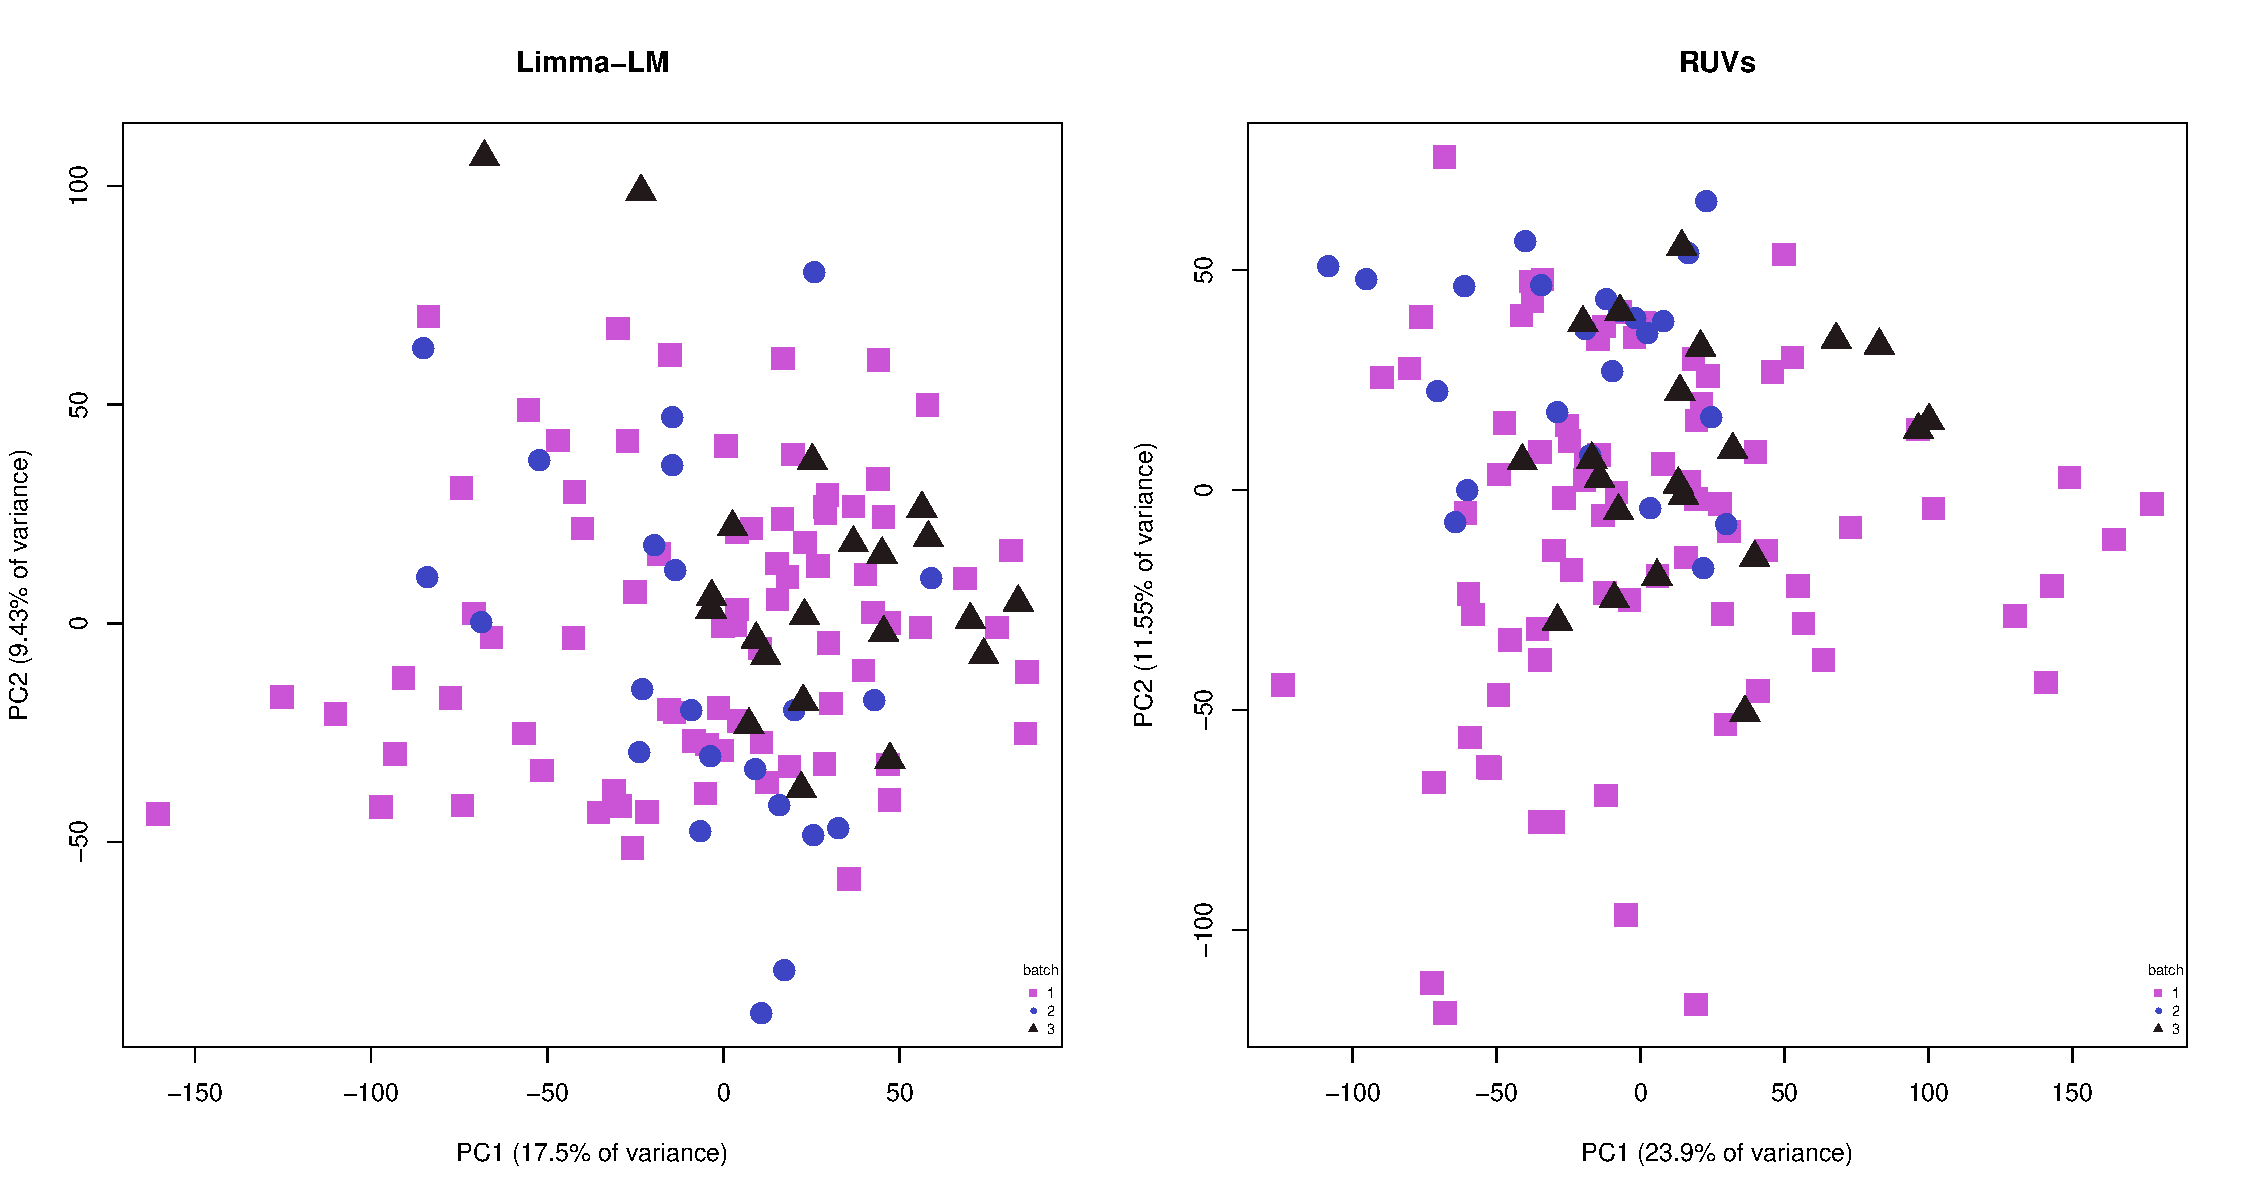
\includegraphics[width=\textwidth,height=\textheight,keepaspectratio]{Figures/PCA_RUVvsLM_FirstDimension.pdf}
\caption{PCA plots of batch-corrected, log2-transformed CPM. The plot on the left is the limma corrected data, generated by the ‘Remove Batch effect’ function from the limma package. The second figure is generated from the RUVs-corrected counts and transformed to the log2 scale. Data corrected by the RUVs method shows more grouping by batch in PC1 and PC2, as well as a higher amount of variance}
\label{fig:RUV vs Limma: PCA by Batch}
\end{figure}


\begin{figure}[htb!]
\centering
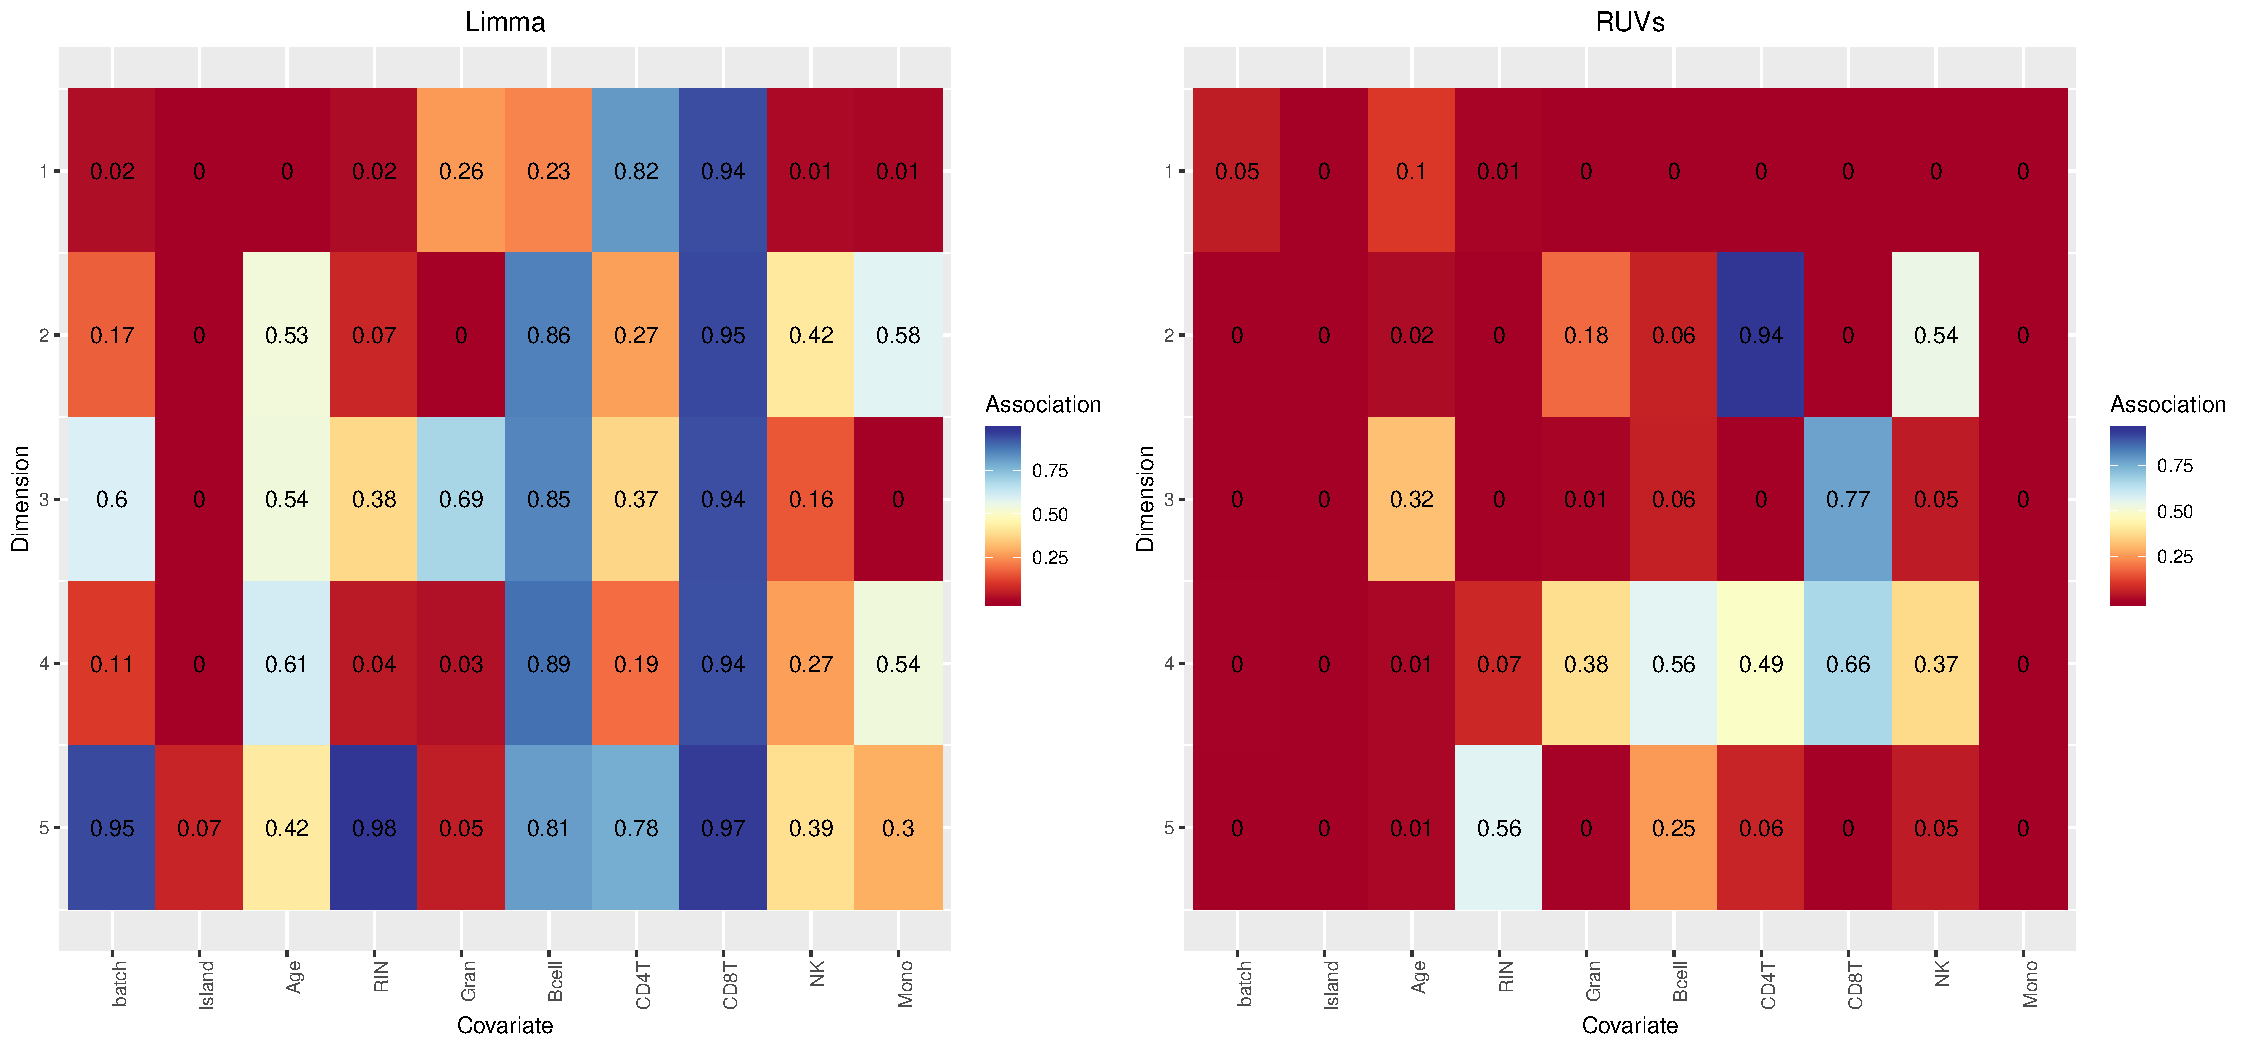
\includegraphics[width=\textwidth,height=\textheight,keepaspectratio]{Figures/Heatmap_SigCovar_RUVvsLM_OnlyCovarInLM.pdf}
\caption{Analysis of variance (ANOVA) between each PCA dimension and covariates included in the design matrix for Limma-corrected and RUVs-corrected data. Count data corrected with the RUVs method can be seen to have a stronger association between most covariates and expression levels.}
\label{fig:RUV vs Limma: Heatmap of Covariates}
\end{figure}

In order to see which method had a higher amount of unexplained variation, I used the package variance Partition which uses a linear mixed model to partition the amount of variance attributable to each variable. The amount of variance explained by each predictor was higher in the linear modelling method, whereas the RUVs correction method had a higher amount of residual variance (Figure 1\ref{fig:Variance Explained}).

\begin{figure}[htb!]
\centering
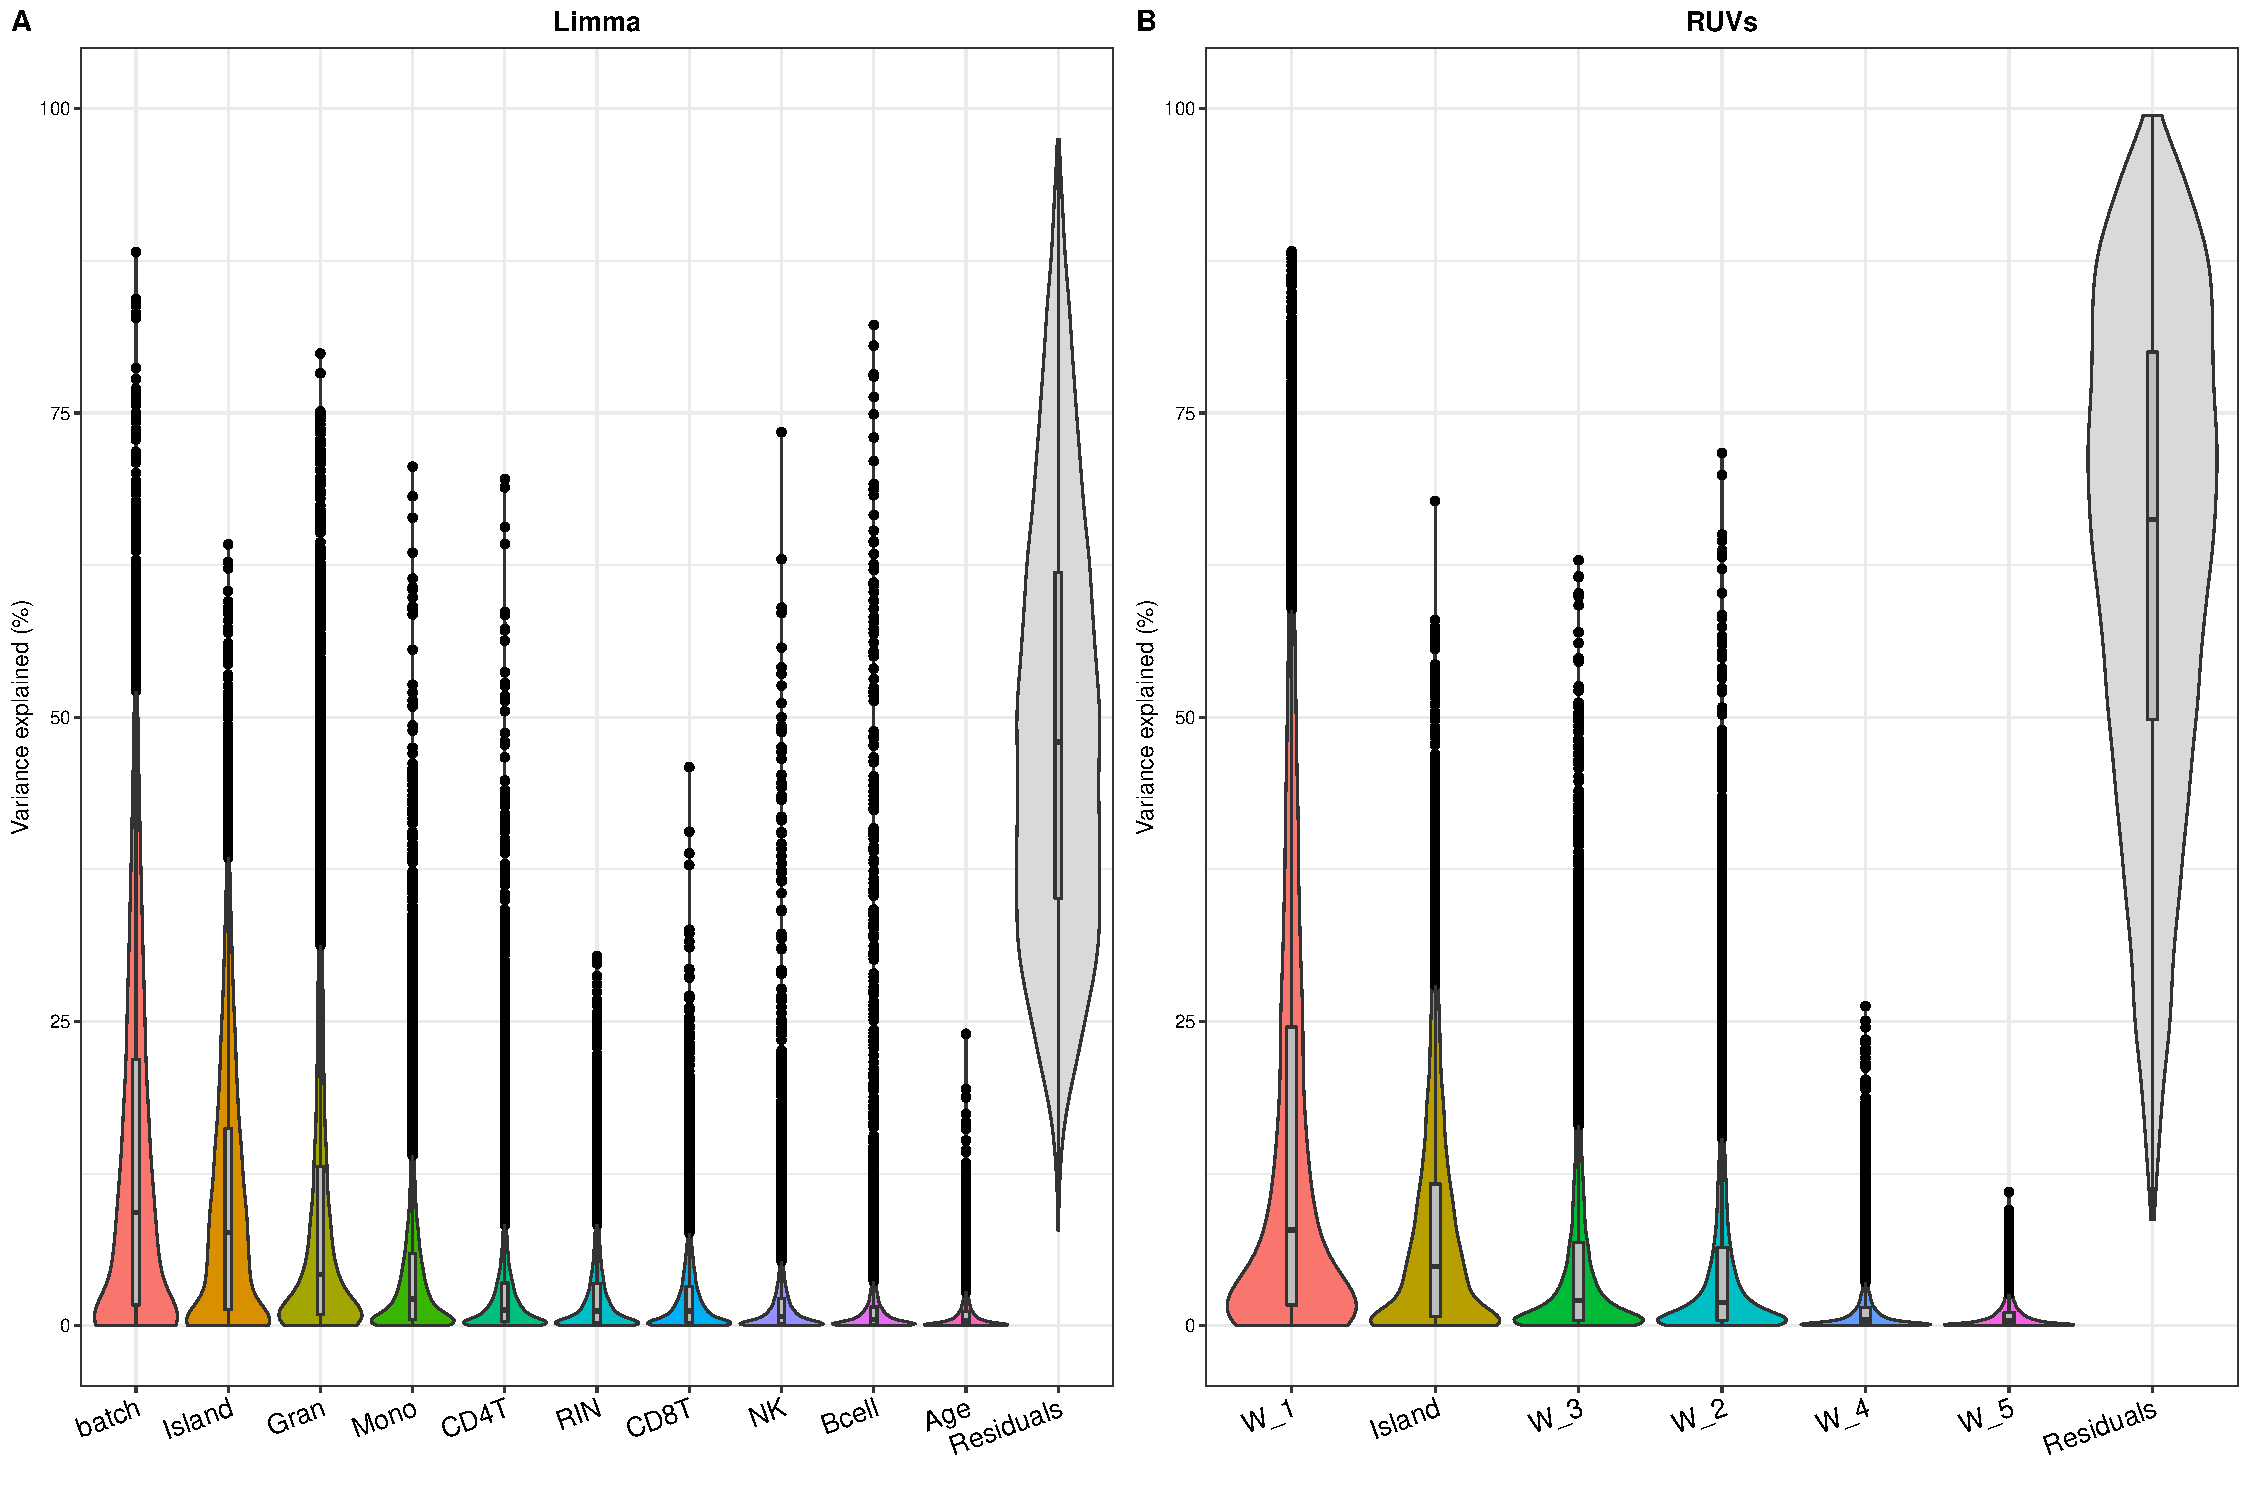
\includegraphics[width=\textwidth,height=\textheight,keepaspectratio]{Figures/VarianceExplained_LMvsRUVs.pdf}
\caption{Total amount of variance explained. variancePartition from the Bioconductor R package was used to assign the amount of variance from each variable in the data. (A) The total amount of variance from all of the covariates shown to influence expression levels, as well as the total amount of residual variation. (B) The total amount of variance explained by each of the five weights calculated by RUVs, as well as island (the covariate of interest) and residual variance.}
\label{fig:Variance Explained}
\end{figure}

Since the batch correction method including known covariates influencing gene expression into a model had less residual variation and a lower association between expression levels and sequencing batch, this method was chosen to correct for batch effects. Furthermore, estimating batch effects through packages such as RUV may introduce incorrect group differences in downstream analyses, particularly when groups are not evenly distributed between the batches (cite: Methods that remove batch effects while retaining group differences may lead to exaggerated confidence in downstream analyses).

\chapter{Results}\label{}

\section{Island structure is maintained in expression profiles}

\begin{figure}[htb!]
\centering
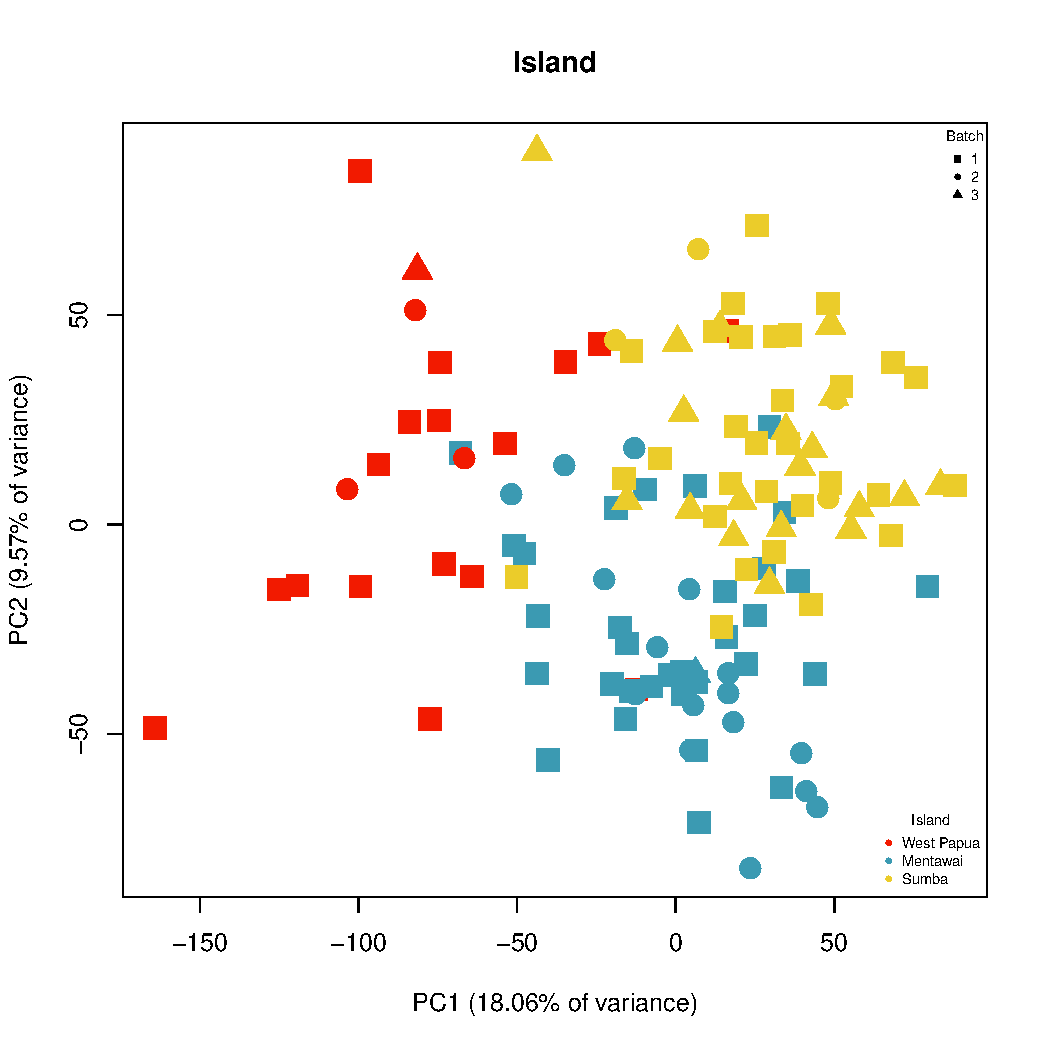
\includegraphics[width=\textwidth,height=\textheight,keepaspectratio]{Figures/pcaresults_Island_RemoveBatchEffect.pdf}
\caption{}
\label{fig:PCA Island}
\end{figure}

\section{Most significantly DE genes are those compared to the Mappi population}

\begin{figure}[htb!]
\centering
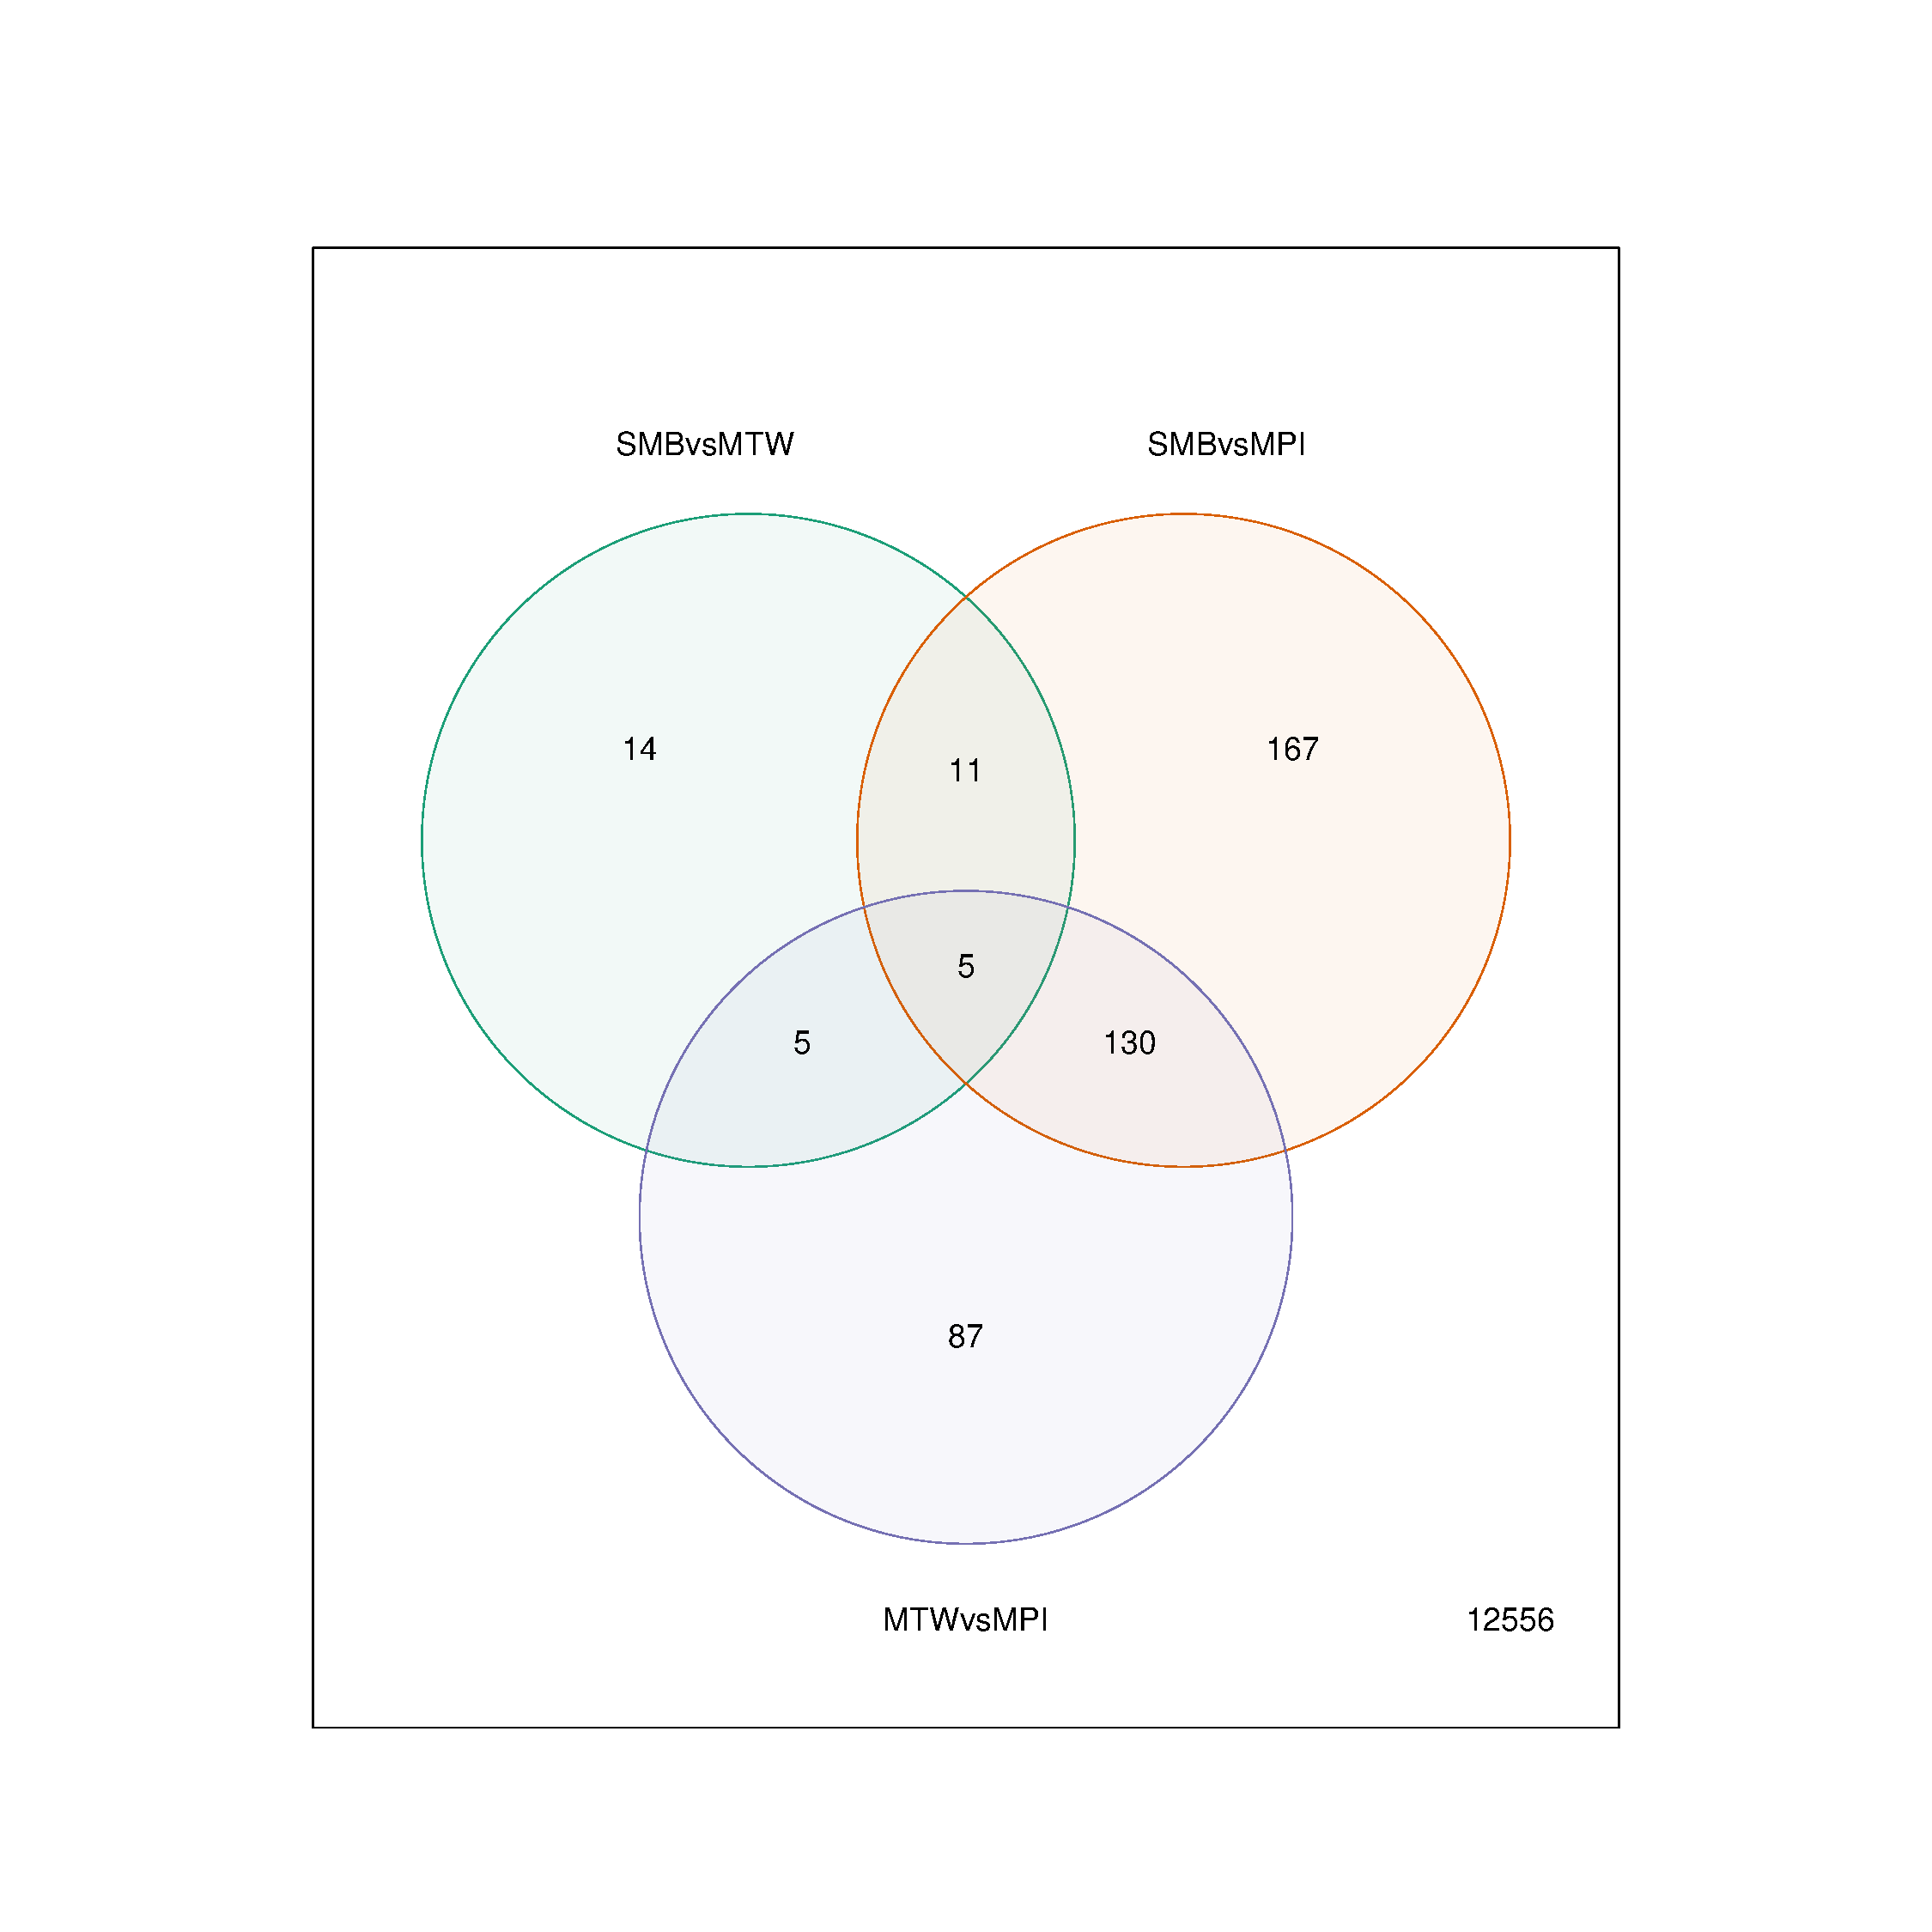
\includegraphics[width=\textwidth,height=\textheight,keepaspectratio]{Figures/vennDiagram_allSigDEGenes_pval01_FDR1_dupCor.pdf}
\caption{Number of significantly DE genes at an FDR of 0.01 and log fold change of one. The number of DE genes that are not in any population comparison are marked in the bottom-right.}
\label{fig:Venn Diagram between Islands}
\end{figure}

\begin{figure}[htb!]
\centering
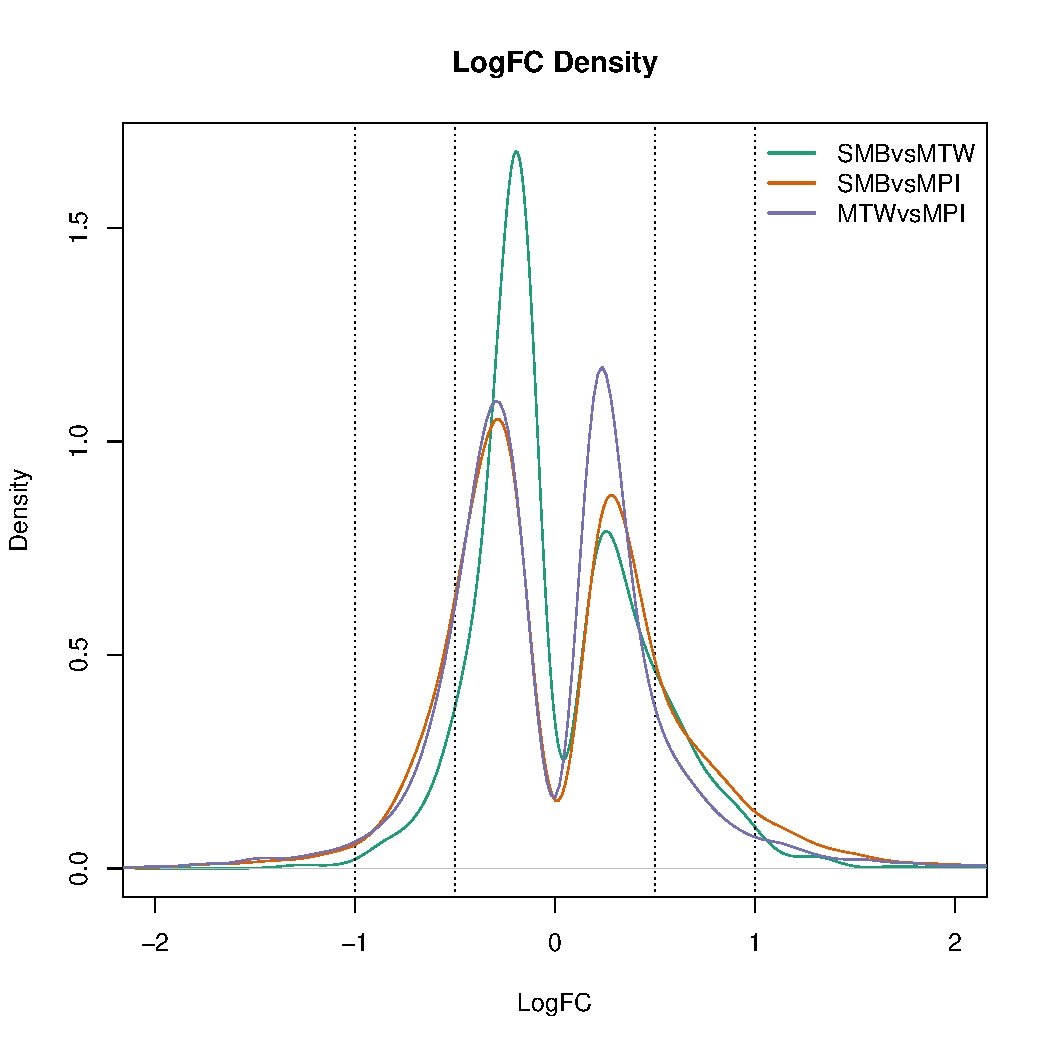
\includegraphics[width=\textwidth,height=\textheight,keepaspectratio]{Figures/log2FC_IslandComparisons_pval01_dupCor.pdf}
\caption{Density of the total number of differentially expressed genes with an FDR of 0.01 for all three population comparisons. Most of the differentially expressed genes with an FDR of 0.01 had an absolute log fold change less than one, particularly in Sumba versus Mentawai.}
\label{fig:LogFC Density}
\end{figure}

\begin{figure}[htb!]
\centering
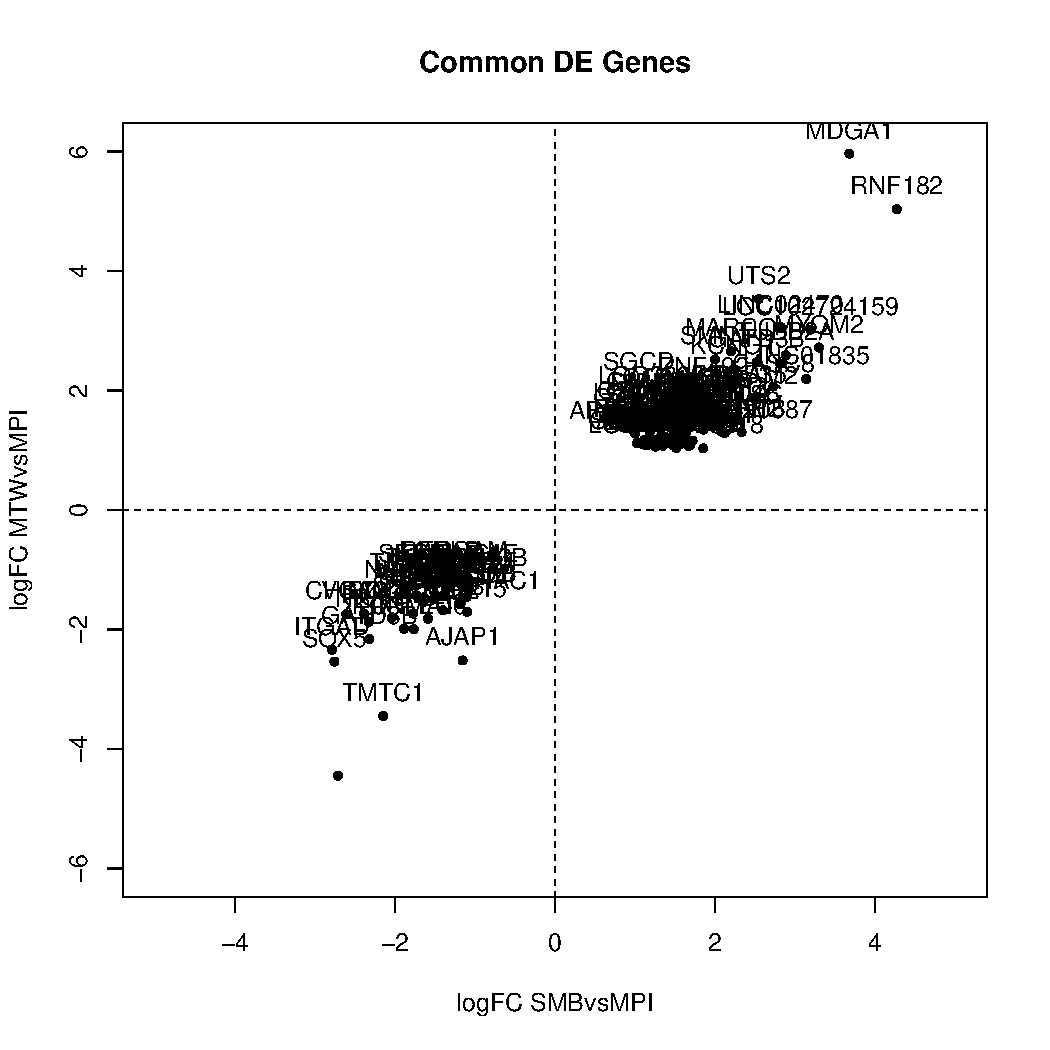
\includegraphics[width=\textwidth,height=\textheight,keepaspectratio]{Figures/logFC_commonMPIgenes_dupCor.pdf}
\caption{Log fold change of differentially expressed genes in Sumba versus Mappi and Mentawai versus Mappi. All significantly DE genes are shown to be both concordantly up or downregulated in both population comparisons.}
\label{fig:LogFC: Mappi vs Others}
\end{figure}

\section{Many DE genes are involved in the immune response}

\begin{figure}[htb!]
\centering
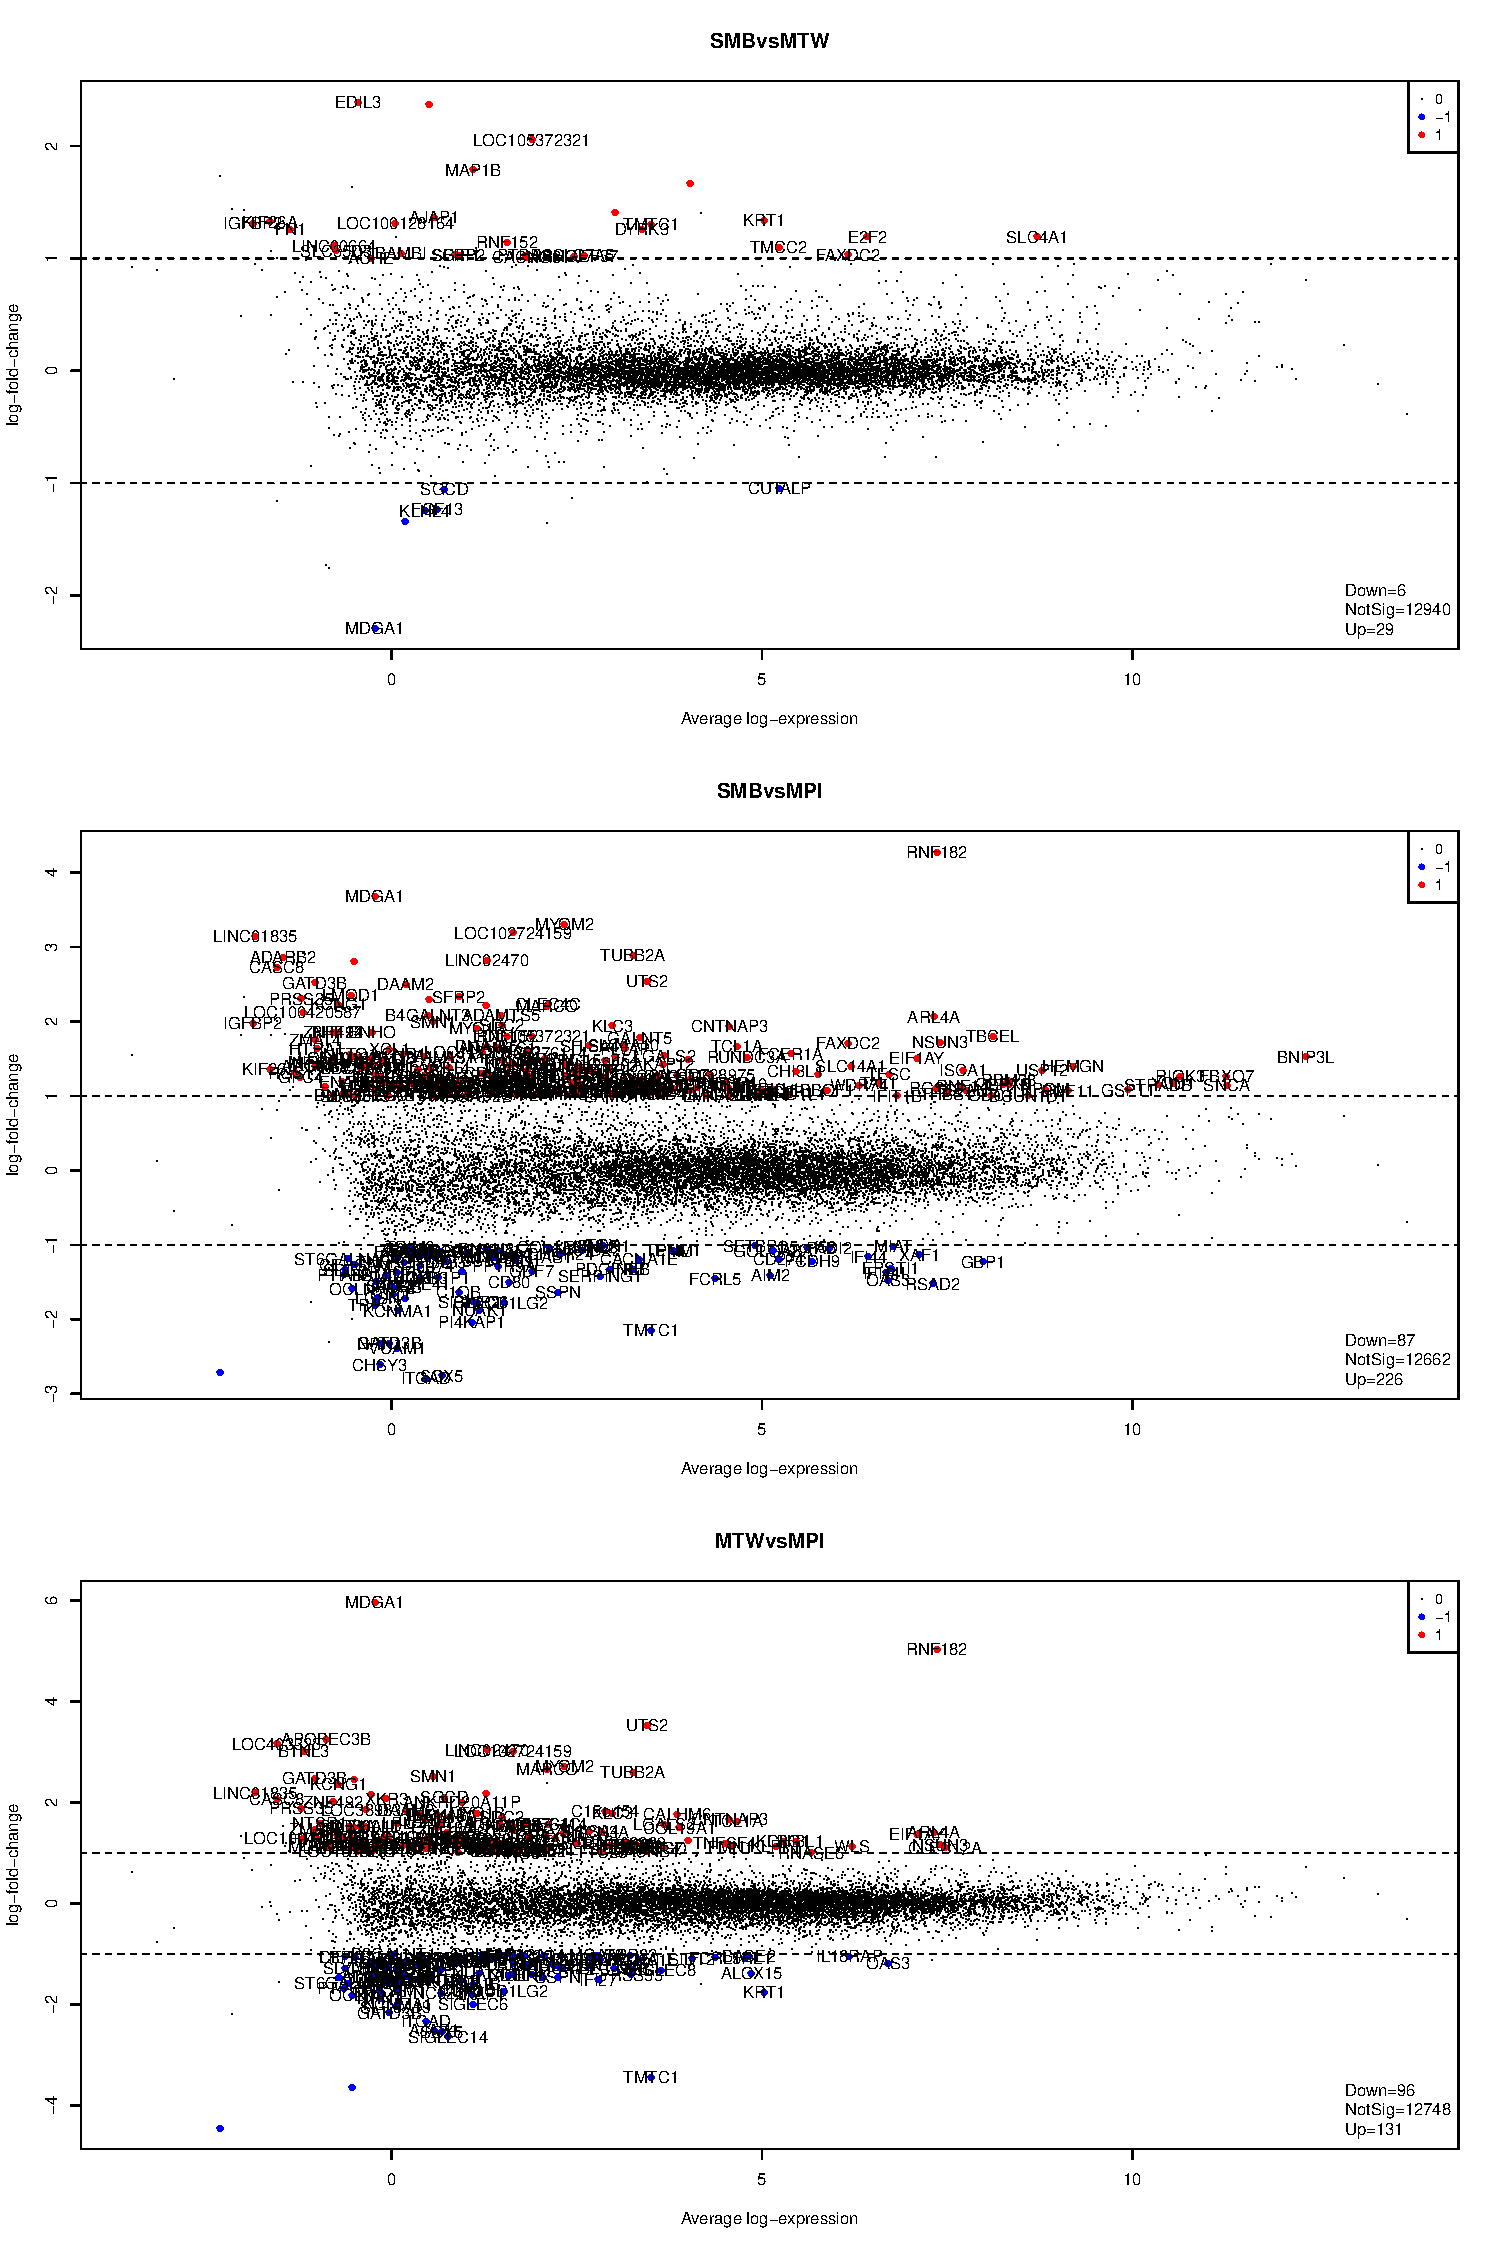
\includegraphics[width=\textwidth,height=\textheight,keepaspectratio]{Figures/MD_Plots_pval01_lfc1_dupCor.pdf}
\caption{Summary of all DE genes with and FDR of 0.01 and a log fold change of one. Each point is the average log2 CPM value fit against the log fold change. Significantly DE genes are labelled for all population comparisons.}
\label{fig:MA Plot}
\end{figure}

\begin{figure}[htb!]
\centering
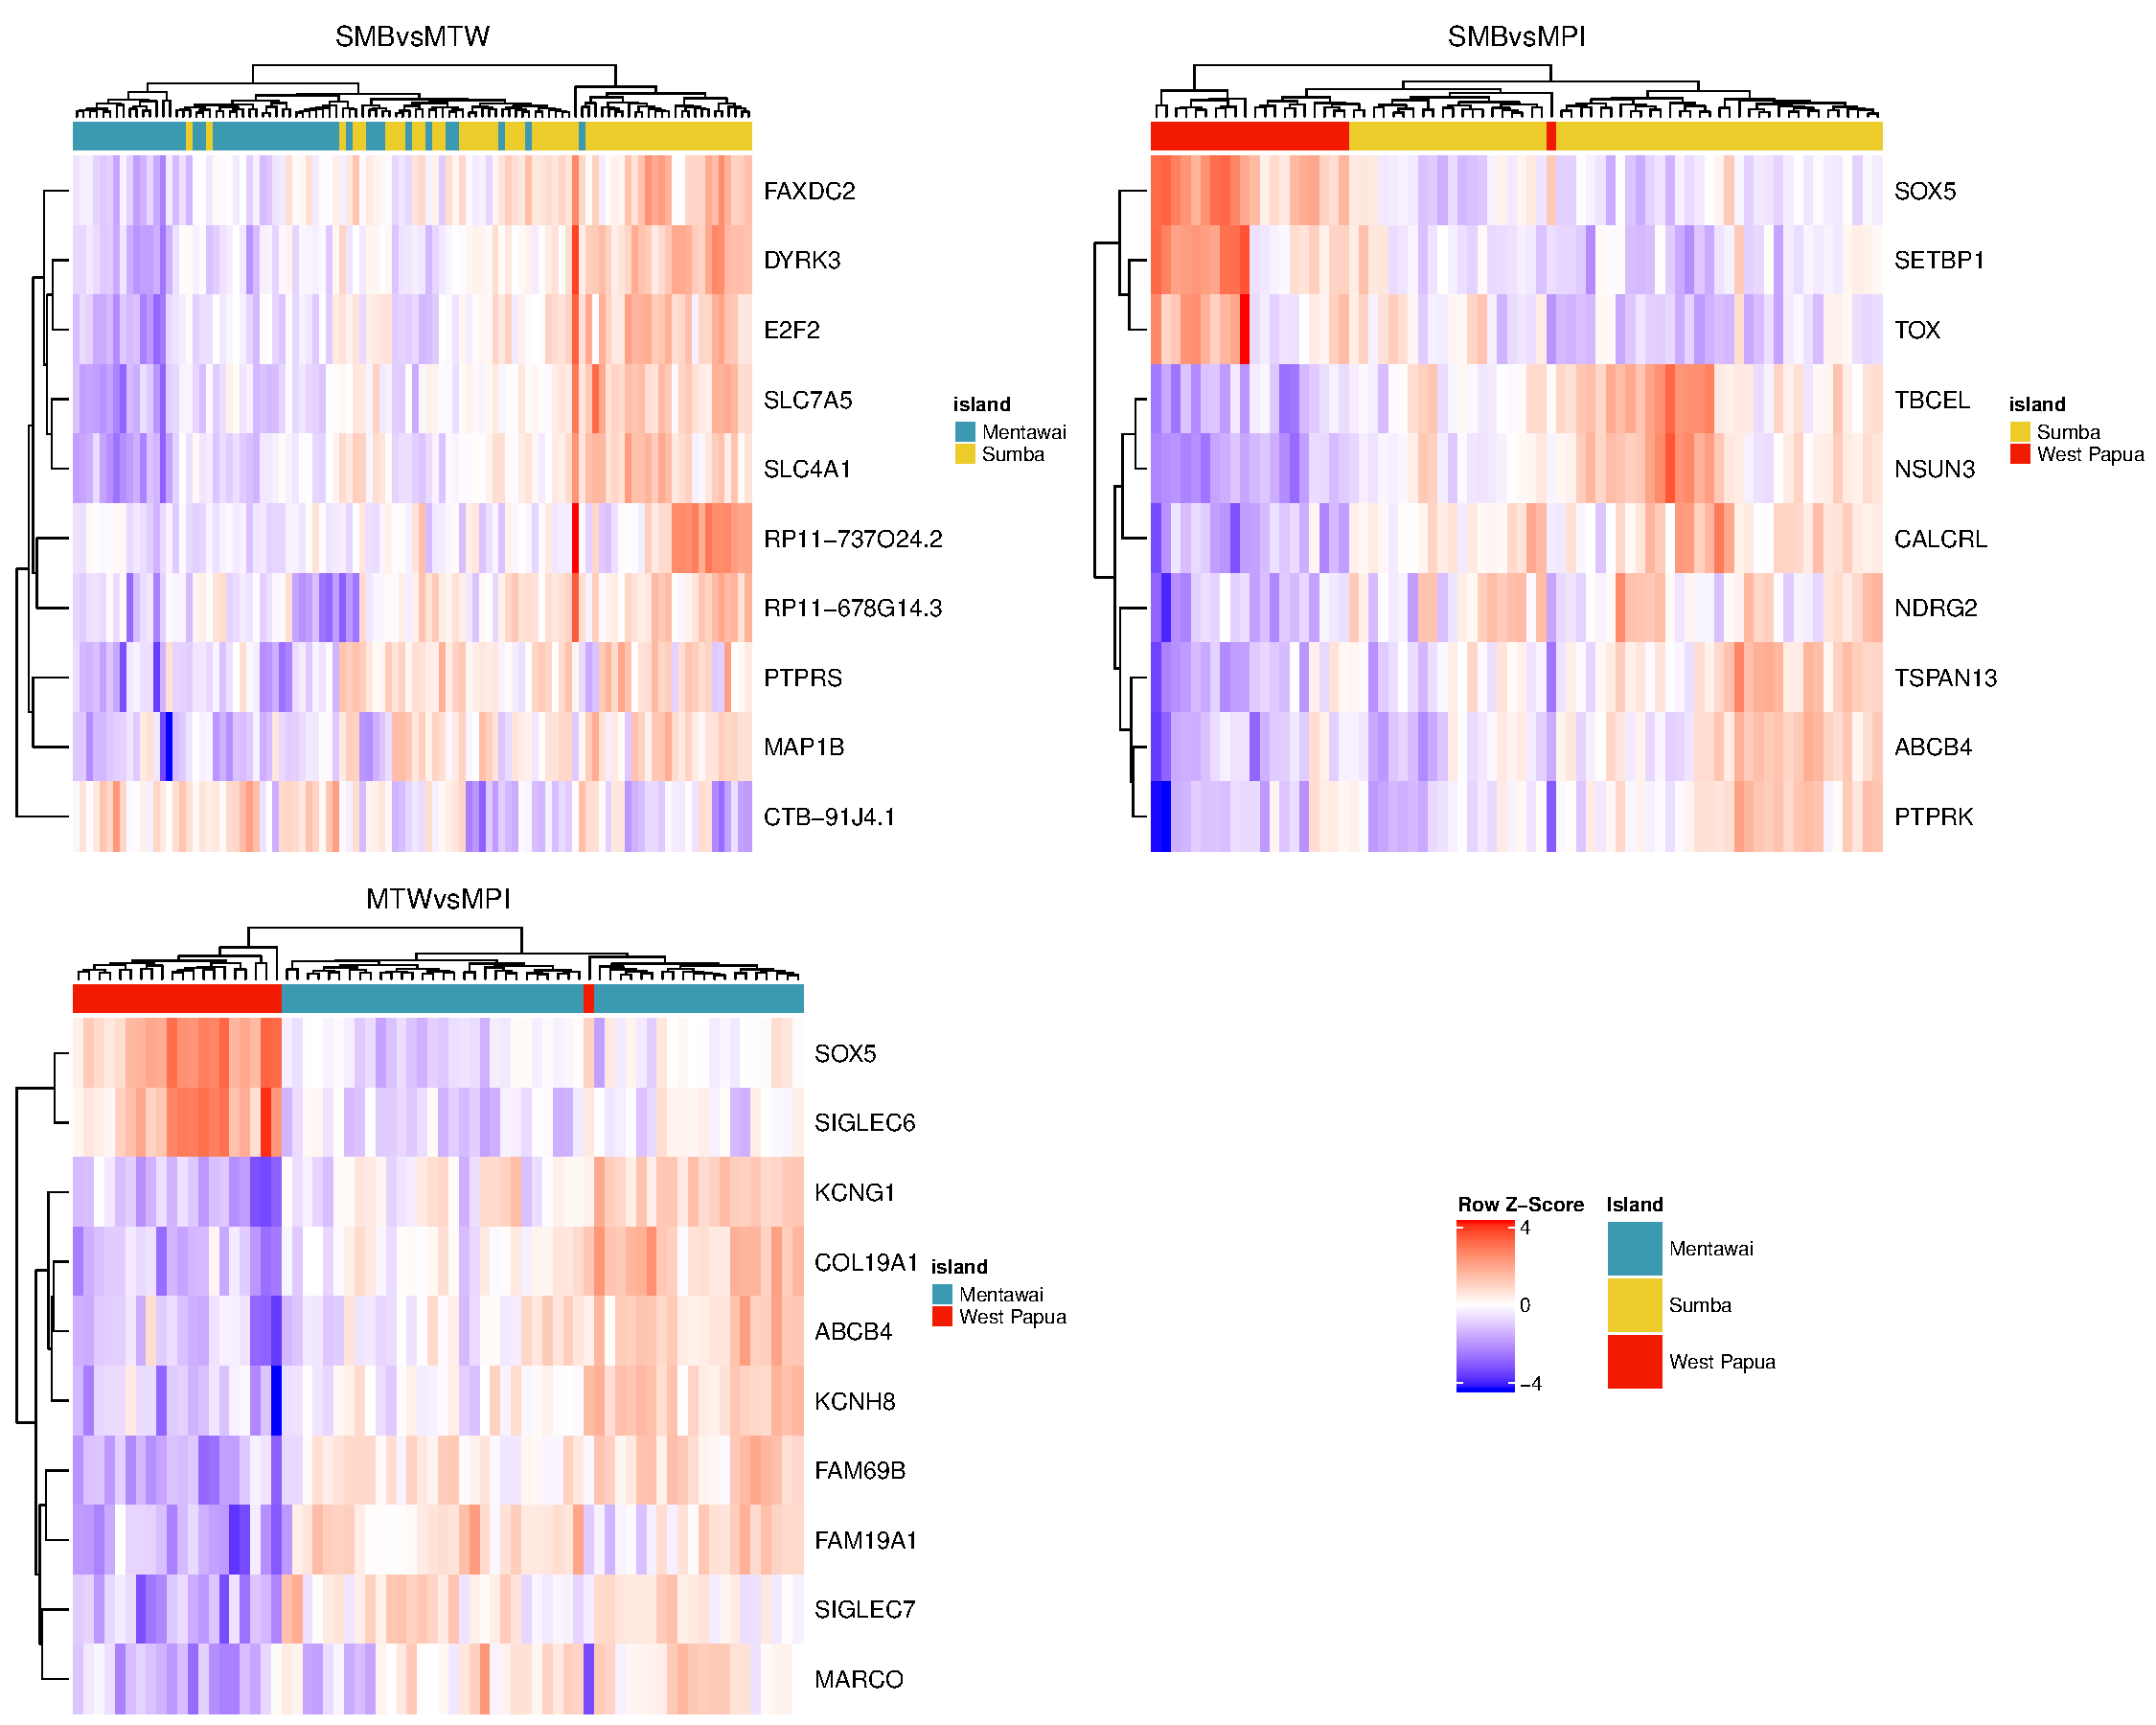
\includegraphics[width=\textwidth,height=\textheight,keepaspectratio]{Figures/HeatmapAllPops_dupCor.pdf}
\caption{Heatmap of log-CPM values for the top ten differentially expressed genes for all population comparisons (sorted by adjusted p-value). Expression across each row is scaled so that the mean expression is zero and the standard deviation is one. Genes with high expression levels are highlighted in red and low expression highlighted in blue. Each column is a sample marked by its island colour (Sumba=yellow, Mappi=red, Mentawai=blue).}
\label{fig:Heatmap Top Genes}
\end{figure}



\section{Gene set testing and pathway analysis}

\begin{figure}[htb!]
\centering
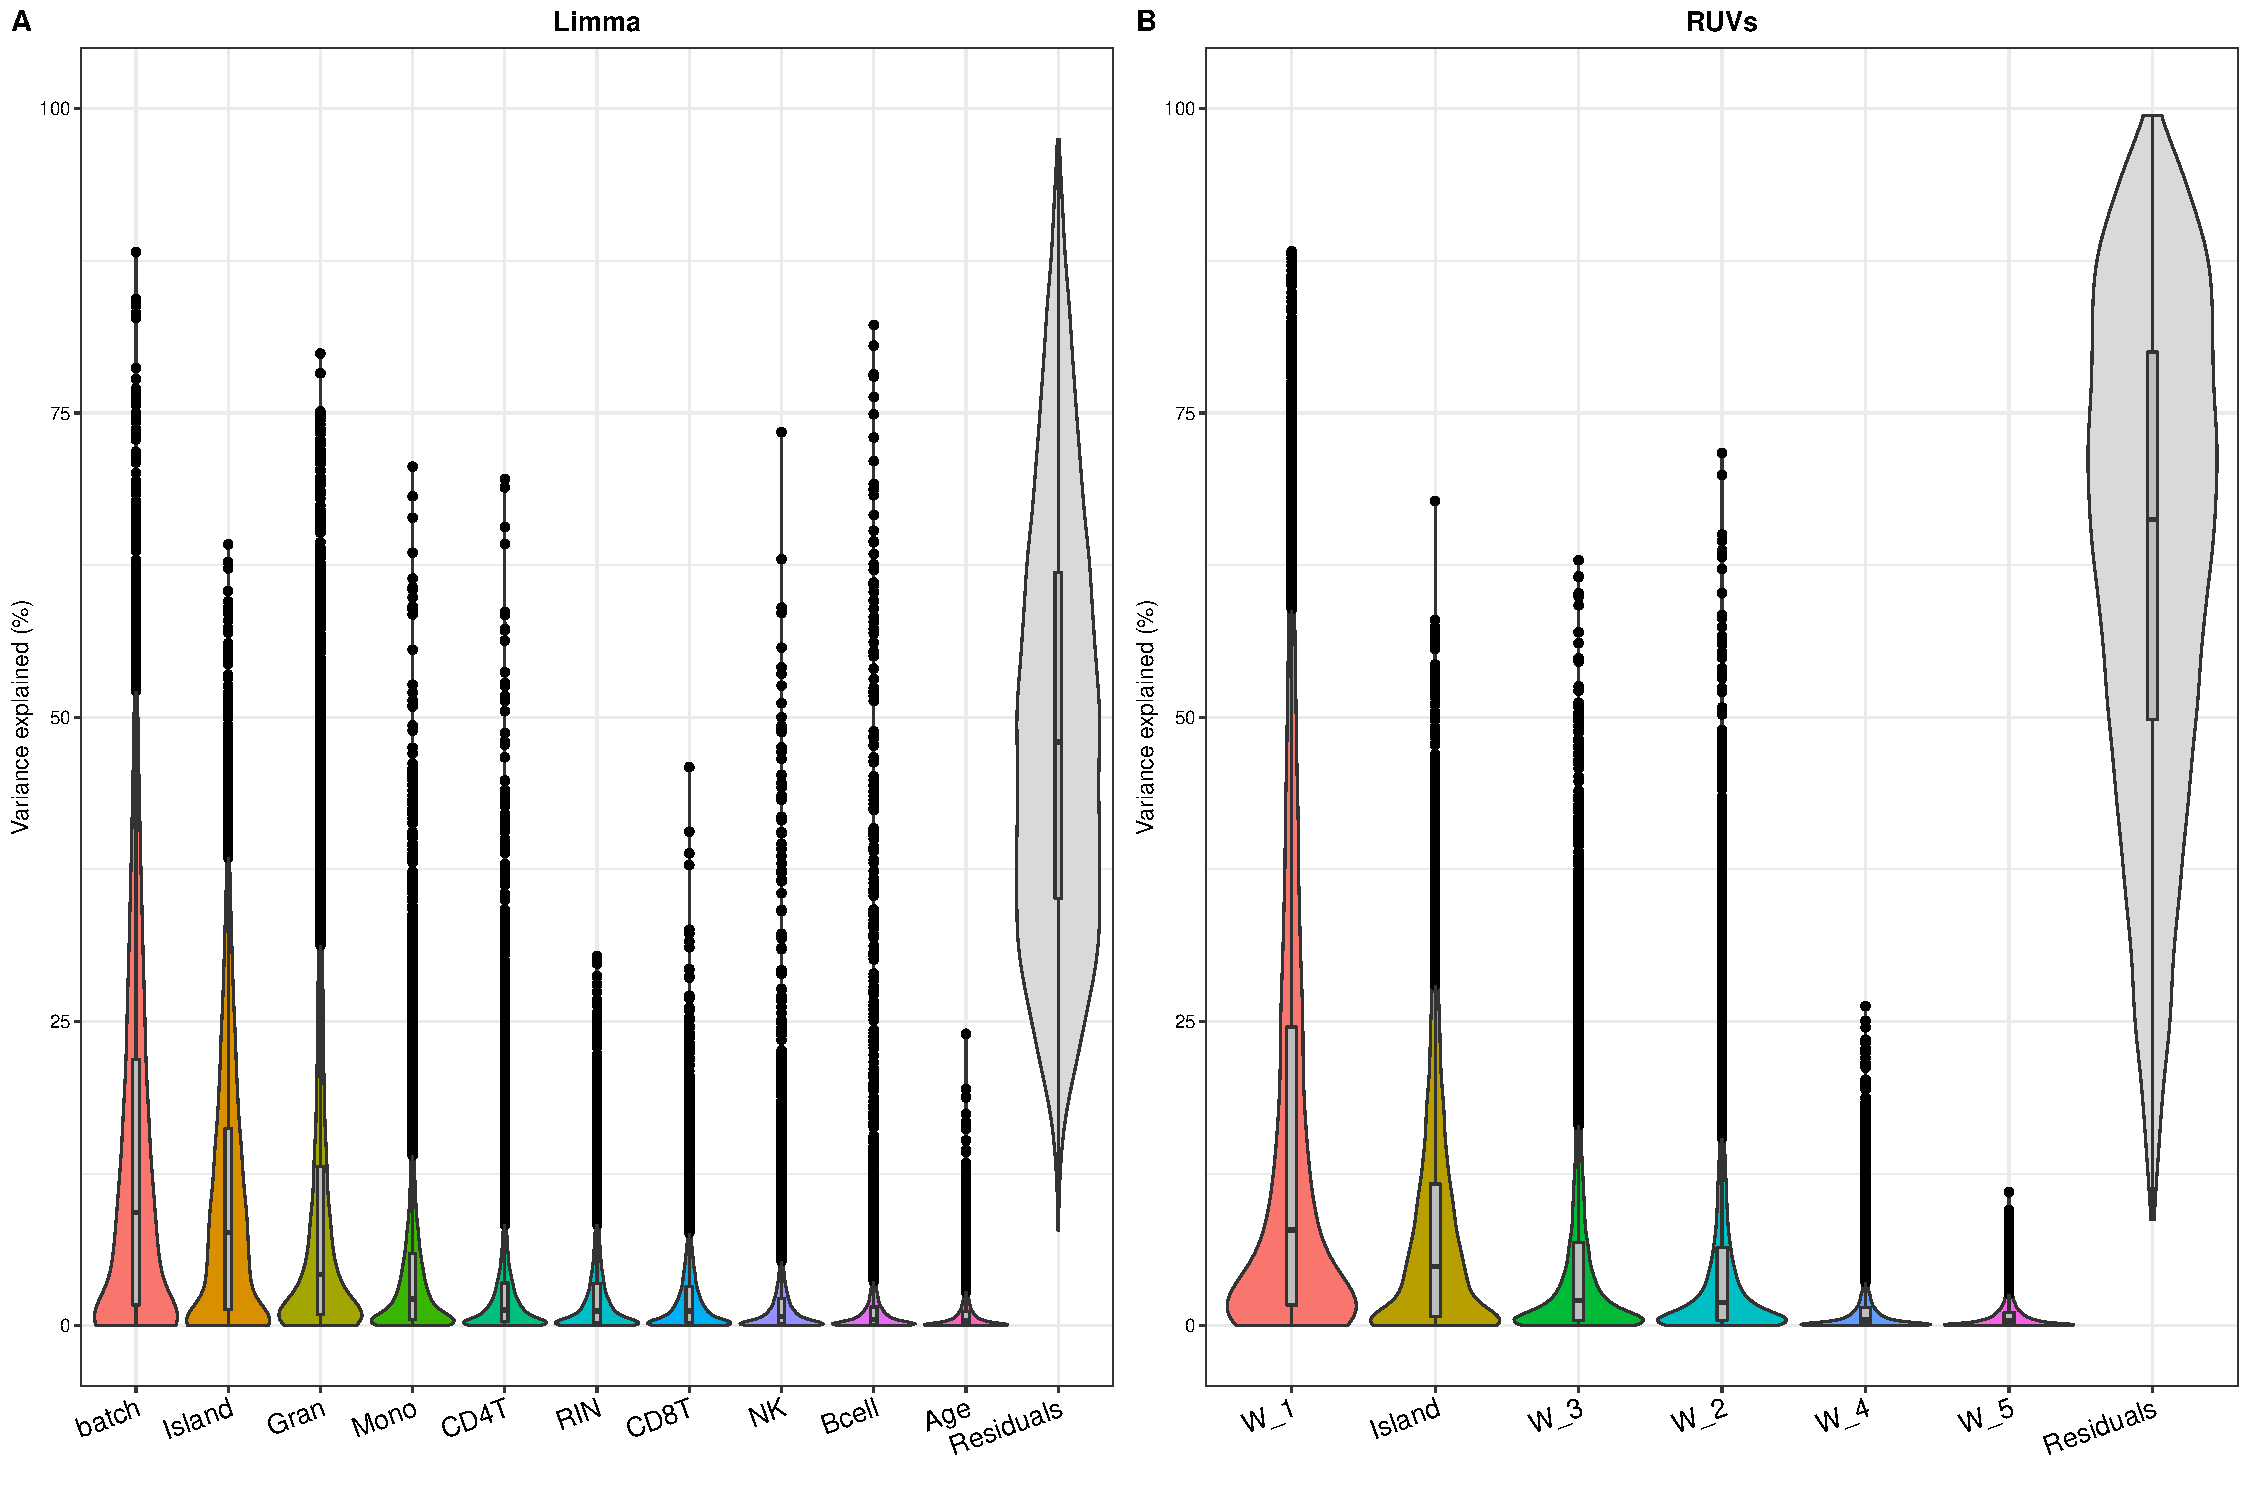
\includegraphics[width=\textwidth,height=\textheight,keepaspectratio]{Figures/VarianceExplained_LMvsRUVs.pdf}
\caption{Total amount of variance explained. variancePartition from the Bioconductor R package was used to assign the amount of variance from each variable in the data. (A) The total amount of variance from all of the covariates shown to influence expression levels, as well as the total amount of residual variation. (B) The total amount of variance explained by each of the five weights calculated by RUVs, as well as island (the covariate of interest) and residual variance.}
\label{fig:Variance Explained}
\end{figure}

\chapter{Discussion}\label{}

\chapter{Supplementary Information}\label{}

\section{Supplementary Figures}

\begin{figure}[htb!]
\centering
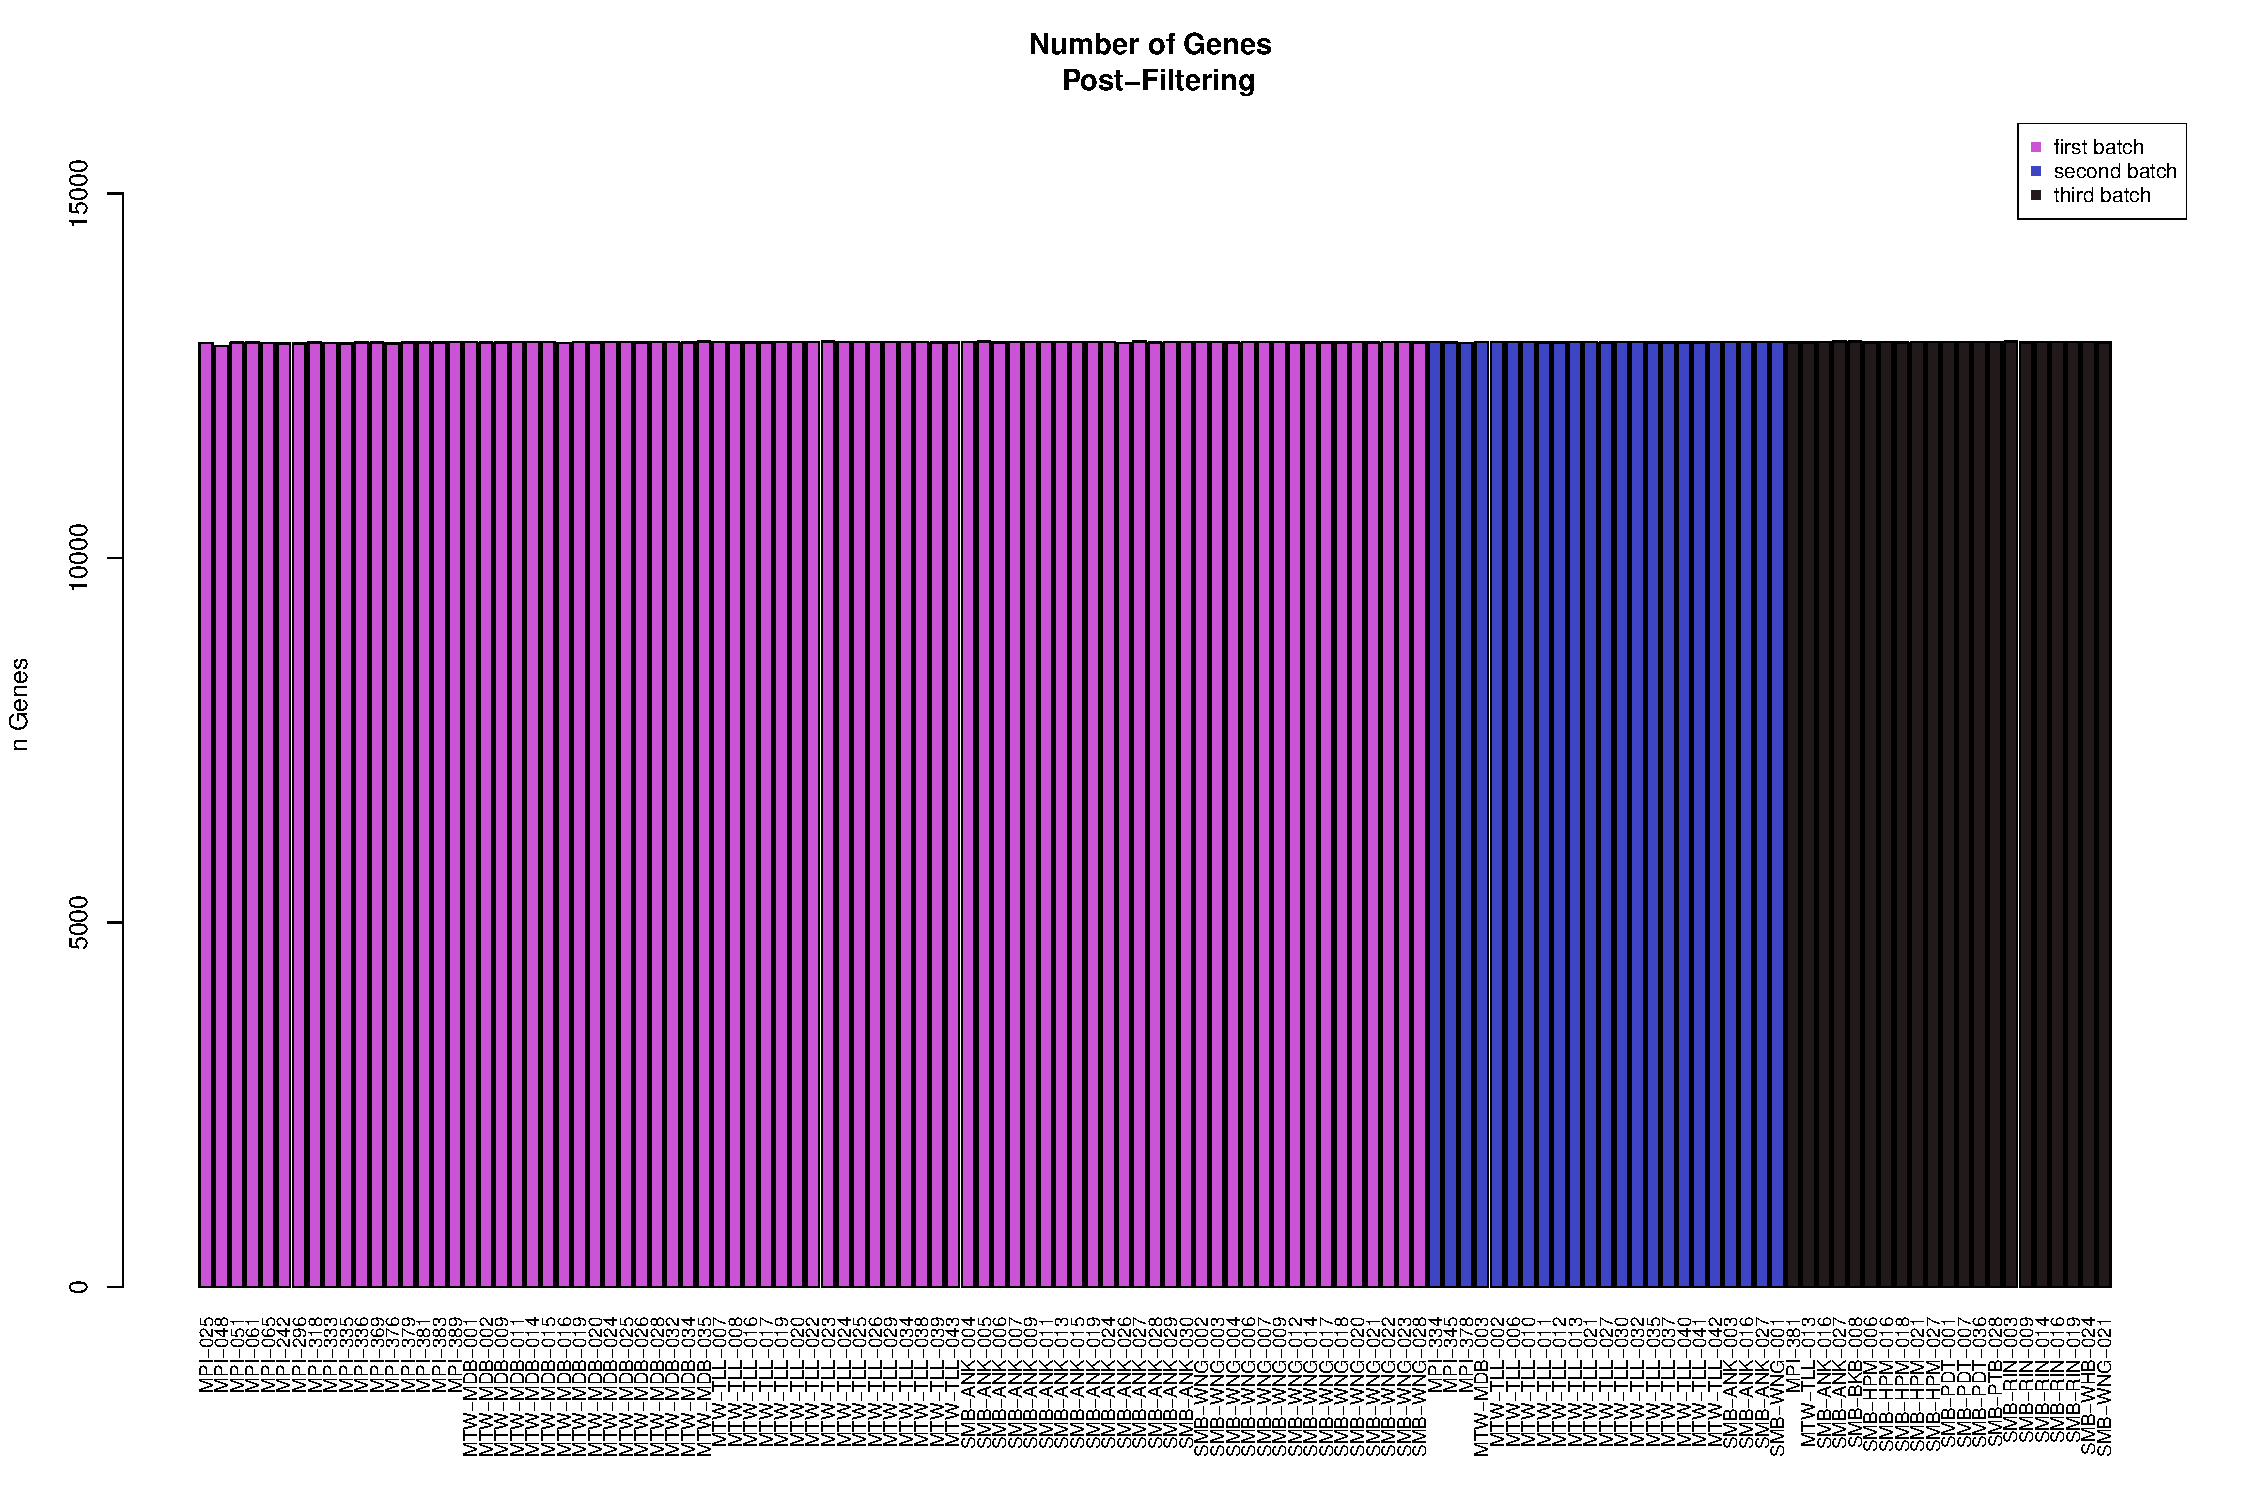
\includegraphics[width=\textwidth,height=\textheight,keepaspectratio]{Figures/nGenes_indoRNA_postFiltering_123Combined.pdf}
\caption{Lowly-expressed genes were removed by only retaining genes expressed at or over 1 in at least on of the island comparisons. This resulted in a total of 12,975 genes (12,914-12,971 genes per sample).}
\label{fig:Total Genes Post Filtering}
\end{figure}


\begin{figure}[htb!]
\centering
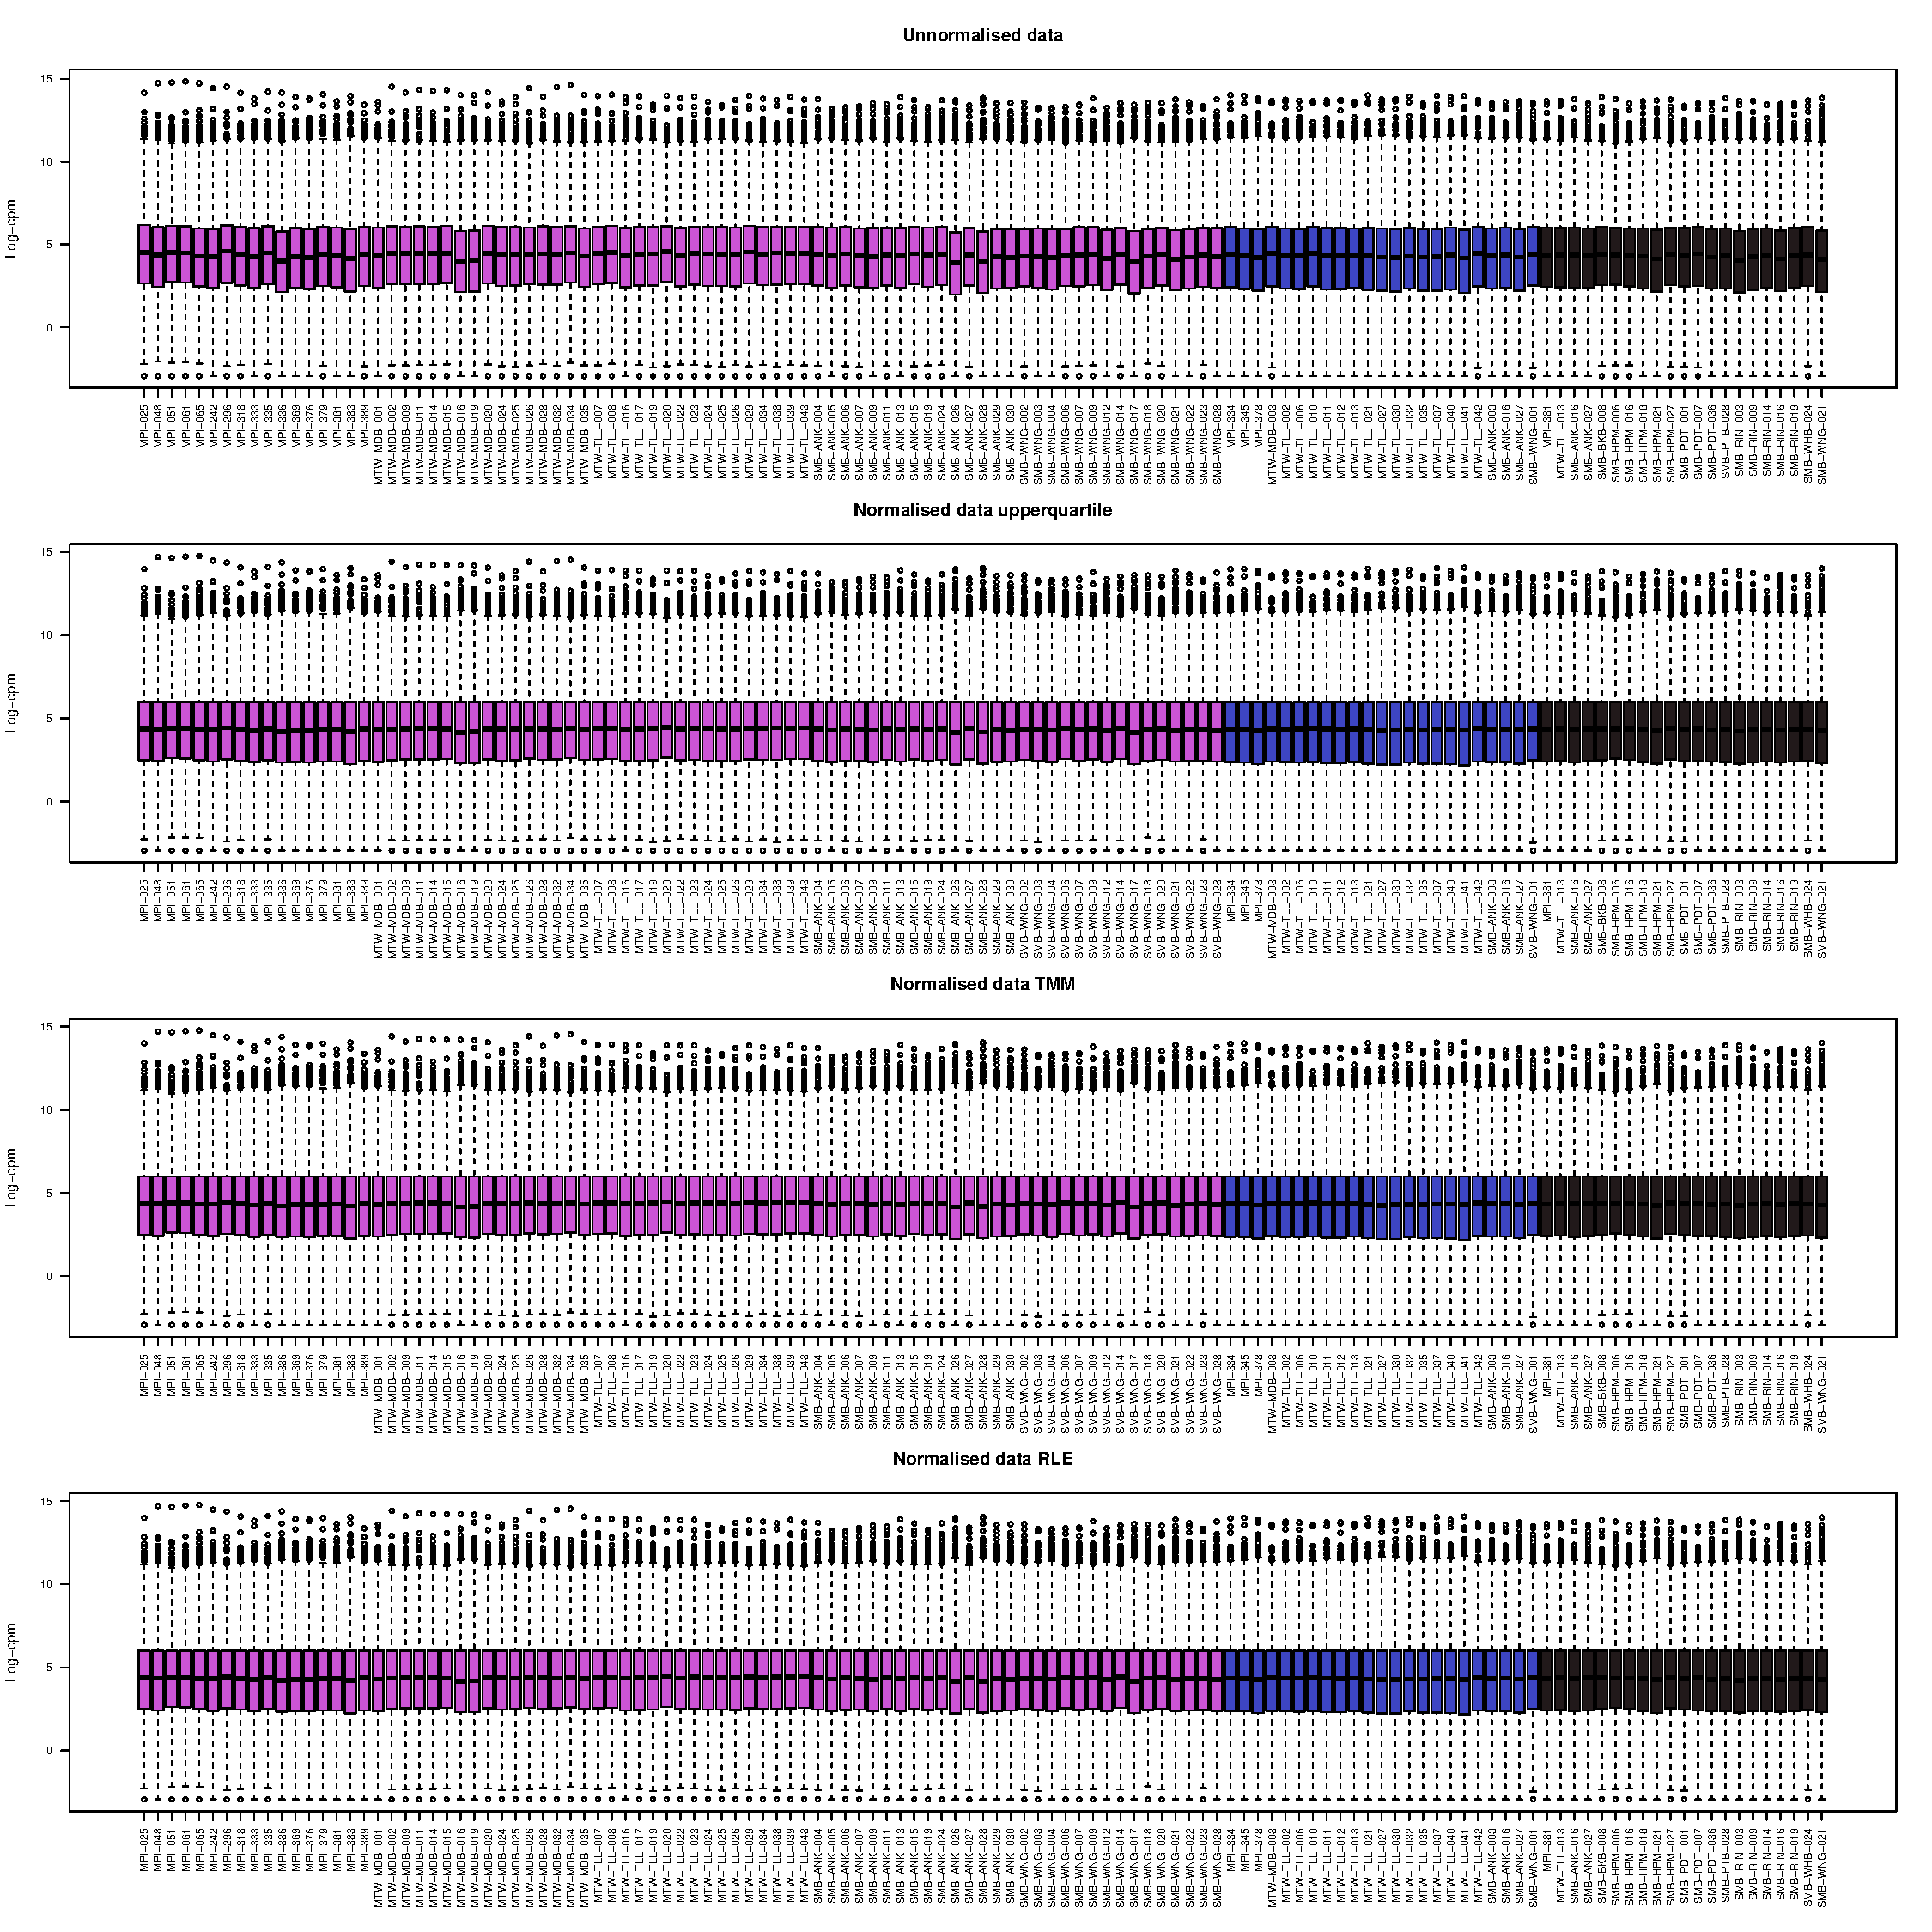
\includegraphics[width=\textwidth,height=\textheight,keepaspectratio]{Figures/NormalisedGeneExpressionDistribution_IndoRNA_all3Methods.pdf}
\caption{Performance of three different normalisation methods on the log2-transformed, filtered data. TMM normalisation was chosen due to its high performance in previous studies.}
\label{fig:Testing Normalisation Methods}
\end{figure}

\section{Supplementary Tables}

\bibliographystyle{plain}
\bibliography{references}
\end{document}
